\input{"AAUImport"/setup/preamble.tex}
\input{"AAUImport"/setup/hyphenations.tex}
% see, e.g., http://en.wikibooks.org/wiki/LaTeX/Customizing_LaTeX#New_commands
% for more information on how to create macros

%%%%%%%%%%%%%%%%%%%%%%%%%%%%%%%%%%%%%%%%%%%%%%%%
% Macros for the titlepage
%%%%%%%%%%%%%%%%%%%%%%%%%%%%%%%%%%%%%%%%%%%%%%%%
%Creates the aau titlepage
\newcommand{\aautitlepage}[3]{%
  {
    %set up various length
    \ifx\titlepageleftcolumnwidth\undefined
      \newlength{\titlepageleftcolumnwidth}
      \newlength{\titlepagerightcolumnwidth}
    \fi
    \setlength{\titlepageleftcolumnwidth}{0.4\textwidth-\tabcolsep}
    \setlength{\titlepagerightcolumnwidth}{\textwidth-2\tabcolsep-\titlepageleftcolumnwidth}
    %create title page
    \thispagestyle{empty}
    \noindent%
    \begin{tabular}{@{}ll@{}}
      \parbox{\titlepageleftcolumnwidth}{
        \iflanguage{danish}{%
          \includegraphics[width=\titlepageleftcolumnwidth]{"AAUImport/figures/aau_logo_da"}
        }{%
          \includegraphics[width=125pt]{"AAUImport/figures/aau_logo_en"}
        }
      } &
      \parbox{\titlepagerightcolumnwidth}{\raggedleft\sf\small
        #2
      }\bigskip\\
       #1 &
      \parbox[t]{\titlepagerightcolumnwidth}{%
      \textbf{Abstract:}\bigskip\par
        \fbox{\parbox{\titlepagerightcolumnwidth-2\fboxsep-2\fboxrule}{%
          #3
        }}
      }\\
    \end{tabular}
    \vfill
    \iflanguage{danish}{%
      \noindent{\footnotesize\emph{Rapportens indhold er frit tilgængeligt, men offentliggørelse (med kildeangivelse) må kun ske efter aftale med forfatterne.}}
    }{%
      \noindent{\footnotesize\emph{The content of this report is freely available, but publication (with reference) may only be pursued due to agreement with the author.}}
    }
    \clearpage
  }
}

%Create english project info
\newcommand{\englishprojectinfo}[8]{%
  \parbox[t]{\titlepageleftcolumnwidth}{
    \textbf{Title:}\\ #1\bigskip\par
    \textbf{Theme:}\\ #2\bigskip\par
    \textbf{Project Period:}\\ #3\bigskip\par
    \textbf{Project Group:}\\ #4\bigskip\par
    \textbf{Participants:}\\ #5\bigskip\par
    \textbf{Supervisor:}\\ #6\bigskip\par
    %\textbf{Copies:} #7\bigskip\par
    \textbf{Page Numbers:} \pageref{LastPage}\bigskip\par
    \textbf{Date of Completion:}\\ #8
  }
}

%Create danish project info
\newcommand{\danishprojectinfo}[8]{%
  \parbox[t]{\titlepageleftcolumnwidth}{
    \textbf{Titel:}\\ #1\bigskip\par
    \textbf{Tema:}\\ #2\bigskip\par
    \textbf{Projektperiode:}\\ #3\bigskip\par
    \textbf{Projektgruppe:}\\ #4\bigskip\par
    \textbf{Deltager(e):}\\ #5\bigskip\par
    \textbf{Vejleder(e):}\\ #6\bigskip\par
    \textbf{Oplagstal:} #7\bigskip\par
    \textbf{Sidetal:} \pageref{LastPage}\bigskip\par
    \textbf{Afleveringsdato:}\\ #8
  }
}

%%%%%%%%%%%%%%%%%%%%%%%%%%%%%%%%%%%%%%%%%%%%%%%%
% An example environment
%%%%%%%%%%%%%%%%%%%%%%%%%%%%%%%%%%%%%%%%%%%%%%%%
\theoremheaderfont{\normalfont\bfseries}
\theorembodyfont{\normalfont}
\theoremstyle{break}
\def\theoremframecommand{{\color{gray!50}\vrule width 5pt \hspace{5pt}}}
\newshadedtheorem{exa}{Example}[chapter]
\newenvironment{example}[1]{%
		\begin{exa}[#1]
}{%
		\end{exa}
}

\newcounter{defcounter}
\setcounter{defcounter}{0}
\newenvironment{hypothesis}{%
\addtocounter{equation}{-1}
\refstepcounter{defcounter}
\renewcommand\theequation{H.\thedefcounter}
\begin{equation}}
{\end{equation}}

\newcounter{subcounter}
\setcounter{subcounter}{0} % Problemet er hvis man f.eks skal lave en ny subhypotese til H7, så vil den første være H.7.3 nu, for. Jo hvis det er casen, så er det no stress
%Ja, men tror du ikke det kun er hyp 5 der får subhyps?
%Ellers laver vi bare en subhypothesis2 command med en ny counter <--- trueeeee
%Nice fix *highfive*
%Nice *fistbump*
%Hvorfor fistbumper du en highfive din retard?
%Shit det var akavet, nu tør jeg ikke tage i grupperummet igen :S
%Nej du må hellere blive væk for evigt
% *græder*
%*griner*
%*grinder*? - nej
%Og så levede de lykkeligt til deres dages ende <- det her

\newenvironment{subhypothesis}{%
%\addtocounter{equation}{0}
\refstepcounter{subcounter} %denne linie incrementer subcounter, tror jeg
\renewcommand\theequation{H.5.\thesubcounter}
\begin{equation}}
{\end{equation}}

% \newcounter{snippetcounter}
% \setcounter{snippetcounter}{0}
% \newenvironment{pythonsnippet}{%
% \addtocounter{figure}{-1}
% \refstepcounter{snippetcounter}
% \renewcommand\thefigure{Code Snippet \thesnippetcounter}
% \begin{figure}[H]
% \begin{cmintedlinenos}[linenos]{python}}
% {\end{cmintedlinenos}\end{figure}}

%\usepackage{subcaption}
\usepackage{booktabs}
\usepackage[norule]{footmisc} %used to remove rule from footnotes
\usepackage{longtable} %used for the semantic rule tables
\usepackage{floatflt,amsmath,amssymb} %used to make the semantic fractions
\usepackage[ligature, inference]{semantic}
\usepackage{graphicx}
\usepackage{caption}
\usepackage{wrapfig, tikz}
\usepackage{floatflt}
%\usepackage{subfig}
\usepackage{afterpage}
\usepackage{listings}

\usepackage{morewrites}

\usepackage{xpatch,letltxmacro}
\usepackage{longtable}
\usepackage{pgfplots}
\usepackage{pdfpages}
\usepackage{lipsum}
\usepackage{pdfpages}
\usepackage{glossaries}
%\usepackage{glossaries-extra}
\usepackage{xcolor}
\usepackage{tabularx}
\usepackage[color, leftbars]{changebar}
\usepackage{multicol}
\usepackage{amssymb}
\usepackage{amsmath}
\usepackage{figsize}
\usepackage{multirow}


\definecolor{OliveGreen}{rgb}{0,0.6,0}
\definecolor{myorange}{rgb}{1.0, 0.63, 0.48}
\definecolor{mygreen}{rgb}{0.74, 0.85, 0.34}
\definecolor{myblue}{rgb}{0, 240, 240}

\setlength\changebarsep{5pt}

\makeglossaries
\loadglsentries{glossaries.tex}

\pgfplotsset{width=10cm,compat=1.9}

\usemintedstyle{}
\newcommand\mynumberformat{\def\FancyVerbFormamtLine##1{{\theFancyVerbLine} ##1}}
\LetLtxMacro{\cmintedlinenos}{\minted}
\let\endcmintedlinenos\endminted
\xpretocmd{\cmintedlinenos}{\setminted{linenos=true}\RecustomVerbatimEnvironment{Verbatim}{BVerbatim}{formatcom=\mynumberformat}{}}{}{}

\LetLtxMacro{\cminted}{\minted}
\let\endcminted\endminted
\xpretocmd{\cminted}{\RecustomVerbatimEnvironment{Verbatim}{BVerbatim}{}}{}{}
\newcommand{\changelocaltocdepth}[1]{%
  \addtocontents{toc}{\protect\setcounter{tocdepth}{#1}}%
  \setcounter{tocdepth}{#1}%
}

\lstset{
 % basicstyle=\itshape,
  xleftmargin=3em,
  literate={->}{$\rightarrow$}{2}
           {α}{$\alpha$}{1}
           {δ}{$\delta$}{1}
           {lambda}{{$\lambda$}}{1}
}
\newcommand\Tstrut{\rule{0pt}{4ex}}         % = `top' strut
\newcommand\Bstrut{\rule[-4ex]{0pt}{0pt}}   % = `bottom' strut
\newcommand{\ldb}{\mathopen{\lbrack\!\lbrack}} 
\newcommand{\rdb}{\mathclose{\rbrack\!\rbrack}}
\newcommand\blankpage{%
    \null
    \thispagestyle{empty}%
    \addtocounter{page}{-1}%
    \newpage}

\usepackage{etoolbox}
\usepackage{hyperref}
\addto\extrasenglish{
    \def\chapterautorefname{Chapter}
    \def\sectionautorefname{Section}
    \def\subsectionautorefname{Section}
    \def\subsubsectionautorefname{Section}
    \def\tableautorefname{Table}
    \def\figureautorefname{Figure}
    \def\algorithmautorefname{Algorithm}
}
\makeatletter
\pretocmd{\part}{\addtocontents{toc}{\protect\addvspace{-8\p@}}}{}{}
\pretocmd{\chapter}{\addtocontents{toc}{\protect\addvspace{-5\p@}}}{}{}
\pretocmd{\section}{\addtocontents{toc}{\protect\addvspace{-6\p@}}}{}{}
\pretocmd{\subsection}{\addtocontents{toc}{\protect\addvspace{-7\p@}}}{}{}
\makeatother

\usepackage{listings}
\usepackage{xcolor}

\definecolor{codegreen}{rgb}{0,0.6,0}
\definecolor{codegray}{rgb}{0.5,0.5,0.5}
\definecolor{codepurple}{rgb}{0.58,0,0.82}
\definecolor{backcolour}{rgb}{0.95,0.95,0.92}

\lstdefinestyle{mystyle}{
    commentstyle=\color{codegreen},
    keywordstyle=\color{magenta},
    numberstyle=\tiny\color{codegray},
    stringstyle=\color{codepurple},
    basicstyle=\ttfamily\footnotesize,
    breakatwhitespace=false,         
    breaklines=true,                 
    captionpos=b,                    
    keepspaces=true,                 
    numbers=left,                    
    numbersep=5pt,                  
    showspaces=false,                
    showstringspaces=false,
    showtabs=false,                  
    tabsize=2
}

\lstset{style=mystyle}

\begin{document}
\pagestyle{empty} %disable headers and footers
\pagenumbering{roman} %use roman page numbering in the frontmatter

%\includepdf[width=1.38\textwidth, pages=-]{Report/WORST.pdf}
\pdfbookmark[0]{Front page}{label:frontpage}%
\begin{titlepage}
  \addtolength{\hoffset}{0.5\evensidemargin-0.5\oddsidemargin} %set equal margins on the frontpage - remove this line if you want default margins
  \noindent%
  \begin{tabular}{@{}p{\textwidth}@{}}
    \toprule[2pt]
    \midrule
    \vspace{0.2cm}
    \begin{center}
    \Huge{\textbf{
      8th Semester Project Title% insert your title here
    }}
    \end{center}
    \begin{center}
      \Large{     
      Subtitle% insert your subtitle here
      }
    \end{center}
    \vspace{0.2cm}\\
    \midrule
    \toprule[2pt]
  \end{tabular}
  \begin{center}
  
    \vspace{12cm}
    {\large
      Project Report%Insert document type (e.g., Project Report)
    }\\
    %\vspace{0cm}
    {\Large
      SW  E21%Insert your group name or real names here
    }

  \end{center}
  \vfill
  \begin{center}
  Aalborg University\\
  Department of Computer Science
  \end{center}
\end{titlepage}
\clearpage
%
\newpage
\pdfbookmark[0]{English title page}{label:titlepage_en}
\aautitlepage{%
  \englishprojectinfo{
    \textit{SW8 Title}%title
  }{%
    8th Semester Project (Mobility) %theme
  }{%
    Fall Semester 2021 %project period
  }{%
    Groupname % project group
  }{%
    %list of group members
    Abiram Mohanaraj, \\
    Cecilie Hyrup Madsen,\\
    Elisabeth Niemeyer Laursen, \\
    Martin Pekár Christensen, \\
    Melanie Selman,\\
    Mikkel Filip Jensen\\
  }{%
    %list of supervisors
    Supervisor
  }{%
    1 % number of printed copies
  }{%
    26th of May, 2021 % date of completion
  }%
}{%department and address
  \textbf{Department of Computer Science}\\
  Aalborg University\\
  \href{http://www.aau.dk}{http://www.aau.dk}
}{
Lorem ipsum dolor sit amet, consectetur adipiscing elit, sed do eiusmod tempor incididunt ut labore et dolore magna aliqua. Pharetra et ultrices neque ornare. A scelerisque purus semper eget duis at tellus at. Duis ut diam quam nulla. Tristique nulla aliquet enim tortor at auctor urna nunc. Aliquam ut porttitor leo a diam sollicitudin tempor id eu. Eget velit aliquet sagittis id consectetur purus ut faucibus. Diam sit amet nisl suscipit adipiscing bibendum est ultricies integer. Enim eu turpis egestas pretium aenean pharetra. Justo nec ultrices dui sapien eget mi proin sed. Elit scelerisque mauris pellentesque pulvinar pellentesque. Sit amet est placerat in egestas erat. Dis parturient montes nascetur ridiculus mus mauris vitae ultricies.
\\Risus nullam eget felis eget nunc lobortis mattis aliquam faucibus. Tincidunt ornare massa eget egestas purus viverra accumsan in. Dictumst vestibulum rhoncus est pellentesque elit. Interdum velit laoreet id donec. Velit sed ullamcorper morbi tincidunt ornare massa. Malesuada bibendum arcu vitae elementum curabitur. Cursus mattis molestie a iaculis. Imperdiet proin fermentum leo vel orci. Ac orci phasellus egestas tellus rutrum tellus pellentesque eu. Vestibulum rhoncus est pellentesque elit ullamcorper dignissim cras tincidunt.
}
%\cleardoublepagehttps://www.overleaf.com/project/5f51e9d829099c000199193c
%\afterpage{\blankpage}%
%\newpage
%Insert Preface text

\section*{Reading Guide}
%
%% MOTIVATION
\todo{Mangler kilde(r).}
There are many reasons why indoor positioning is worth exploring. Since \gls{gps} are not accurate enough in terms of indoor navigation, the indoor positioning can be used for several different occasions, for instance indoor navigation, location-based notifications, and optimisation of work efficiency.

Indoor navigation could be used for helping the user navigate through office buildings, airports, hospitals etc. This could help users save time and give them a better experience. When the location of the user is known, it is also possible to send them messages based on their location in the airport, store etc. For instance, you could send them a message about an offer on a product when you can see that they are in the duty-free shop in the airport. 

By using indoor location, you could also gain insight into the movement behaviour of people in a certain place. With this information, you could for instance see if your staff always takes the shortest path, or if there are areas of your store that people do not visit. With this information, we could create a more intuitive architecture of our buildings.\cite{IPSMapsPeople}
%https://blog.mapspeople.com/mapsindoors/indoor-positioning-101
%\newpage

\cleardoublepage
\pdfbookmark[0]{Contents}{label:contents}
\pagestyle{fancy} %enable headers and footers again
\pagenumbering{roman}

\setcounter{tocdepth}{1}
\tableofcontents
%\afterpage{\blankpage}

\chapter*{Preface}
Insert Preface text

\section*{Reading Guide}


\renewcommand{\glsgroupskip}{}
\printglossaries
\newpage\pagenumbering{arabic}

\part{Introduction \& Analysis}

\chapter{Introduction}
% MOTIVATION
\todo{Mangler kilde(r).}
There are many reasons why indoor positioning is worth exploring. Since \gls{gps} are not accurate enough in terms of indoor navigation, the indoor positioning can be used for several different occasions, for instance indoor navigation, location-based notifications, and optimisation of work efficiency.

Indoor navigation could be used for helping the user navigate through office buildings, airports, hospitals etc. This could help users save time and give them a better experience. When the location of the user is known, it is also possible to send them messages based on their location in the airport, store etc. For instance, you could send them a message about an offer on a product when you can see that they are in the duty-free shop in the airport. 

By using indoor location, you could also gain insight into the movement behaviour of people in a certain place. With this information, you could for instance see if your staff always takes the shortest path, or if there are areas of your store that people do not visit. With this information, we could create a more intuitive architecture of our buildings.\cite{IPSMapsPeople}
%https://blog.mapspeople.com/mapsindoors/indoor-positioning-101

\chapter{Problem Analysis}
%\subsection{Motivation}
%\todo{RETTTELSER HER.}
%There are many reasons why indoor positioning is worth exploring. Indoor positioning can be used for several different occasions, for instance indoor navigation, location-based notifications, and optimisation of work efficiency. 
%Indoor navigation could be used for helping the user navigate through office buildings, airports, hospitals etc. This could help users save time and give them a better experience. When the location of the user is known, it is also possible to send them messages based on their location in the airport, store etc. For instance, you could send them a message about an offer on a product, when you can see that they are in the duty-free shop in the airport. 
%By using indoor location, you could also gain insight into the movement behaviour of people in a certain place. With this information, you could for instance see if your staff always takes the shortest path, or if there are areas of your store that people do not visit. With this information, we could create a more intuitive architecture of our buildings.\cite{IPSMapsPeople}
%https://blog.mapspeople.com/mapsindoors/indoor-positioning-101

\textit{When estimating indoor locations, it is relevant to investigate the problem of accurately making these estimates and what an indoor positioning system is, which will be covered in this chapter. For this project, we have chosen to participate in a competition about predicting indoor locations held by the companies Microsoft and XYZ10 on the Kaggle platform. A dataset is provided for the purpose of determining positions, which we will be using for our project. The dataset contains measures from several different sensors and actuators over a variety of buildings and floor levels. Lastly, the different possible existing positioning methods will be covered.}
\section{Indoor Positioning}
In outdoor environments, we rely on satellite-based positioning systems, such as \gls{gps}. \gls{gps} is a U.S utilization that is used by both civilians and the military. To get accurate positioning, navigation and timing services, different components are used: \cite{GPSofficial}

\begin{itemize}
    \item Space component is operated by satellites that transmit signals to users on geographical locations and timestamps. 
    \item Control component consists of different elements: 
    \begin{itemize}
        \item Monitor Stations tracks the \gls{gps} satellites as they pass and feed observations to the Master Control Station. 
        \item Master Control Station computes precise locations of the satellites.
        \item Ground Antennas communicate with satellites. 
    \end{itemize}
    \item User component consists of \gls{gps} receivers or transmitters, including telematic devices, smartphones and etc. 
\end{itemize}

However, the issue with \gls{gps} is that it looses its accuracy when used indoor due to the device not being in line of sight, meaning the device does not have a clear sight to the sky. This is needed for the satellite to place a more accurate position\cite{GPSofficial}. This is due to the reason that signals cannot penetrate through materials, such as glass, brick, metal, etc.\cite{GPSofficial}. \gls{gps} signals are also classified as part of \gls{uhf}, which results in another problem as in an indoor environment, there are potential sources of \gls{uhf} signals which can interfere with the \gls{gps} signal. For example, TV antenna signals can interfere with \gls{gps} signals\cite{GPSofficial}.
This is the reason why we need other technologies when we want to estimate the indoor location. \gls{ips} is a term which covers different technologies that use mobile devices to exploit their physical location. %After an \gls{ips} is developed, it is possible to make use of location-based services.

%https://blog.mapspeople.com/mapsindoors/indoor-positioning-101%
%https://blog.mapspeople.com/mapsindoors/indoor-positioning-101
\section{Application of Sensors and Actuators}\label{sec:actuator_sensor} 
%In this section, we briefly describe the sensors and actuators available in the Kaggle competition for measuring indoor positions. Furthermore, we present the advantages and disadvantages of using these sensors and actuator.

In this section, we briefly describe the commonly used sensors and actuators that can be used in \gls{ips}, along with examples of systems making use of them, their advantages and disadvantages. 

A wide range of technologies are available for \gls{ips}s, that either make use of the sensors in the mobile device or external devices. The phone itself provides \gls{imu} sensor, microphone, cameras and more, all of which are useful for \gls{ips}s. External devices include Wi-Fi router, Bluetooth beacons, \gls{rfid} tags, ultrasound transmitters and more.

%\subsection{Sensors and Actuators Overview}
%subsection{External Devices}

%When using WiFi signals, the users position is calculated based on the strength of the Wi-Fi signals.

%Also, one of the most widely used technologies is \gls{ble} beacons. They, like Wi-Fi routers, send a signal in a radius of 10-30 meters, and then use the Bluetooth signals to position the user.

%A third alternative is using \gls{uwb} transceiver which transmits signals from antennas.

\subsection{Wi-Fi} \label{sec:WiFi}
%Using Wi-Fi routers to measure distance, one can use different techniques, such as \gls{toa}, \gls{tdoa} or \gls{rss}. 
A popular technique for using Wi-Fi is \gls{rss}. An \gls{rssi} is an integer in the range of 0 to 255 that represents the strength of a signal in \gls{dbm}.\cite{RSSIWiFiDistance, RSSIMeasurement}
\gls{rssi} from Wi-Fi routers enable computing the position of a receiver device using triangulation or trilateration, as long as at least three Wi-Fi routers are within range, which will be described in \textbf{\autoref{sec:triangulation}}.
Also, \gls{rssi} from Wi-Fi beacons can be used in fingerprinting, a unique identification of a location, which will be described in \textbf{\autoref{sec:scene_analysis}}\cite{HabilitationThesis}.

One of the advantages of using Wi-Fi is that Wi-Fi is already integrated in many buildings, so it will be easy to implement this solution, and most mobile devices are equipped with Wi-Fi sensors.
A disadvantage of Wi-Fi routers is that they lack in precision and function ideally when there is no obstruction to its signal - for instance walls, furniture, or people. Even when there is no obstruction, Wi-Fi routers will still only have an accuracy of 10-20 meters.\cite{oriient}

Using Wi-Fi for indoor positioning is not as commonly used as Bluetooth due to its low accuracy. However, Skyhook have implemented a Wi-Fi based solution for use in urban areas\cite{skyhook}. The solution is mainly based on fingerprinting, and reaches an accuracy of 10-20 meters outdoors. However, in indoor environments, the system has an accuracy of 30-70 meters. Another solution is provided by Ekahau that is based on a combination of fingerprinting and track history. Their solution reaches an accuracy of around 7 meters in indoor environments.\cite{HabilitationThesis}

%We will probably experiment with Wi-Fi, since it is already widely integrated in buildings and is therefore a cost-effective method. 
%Wi-Fi data is also provided by the dataset at Kaggle, mentioned in \textbf{\autoref{sec:kaggleComp}}.

\subsection{Bluetooth Beacons}
In order to determine the location of a device using Bluetooth beacons, the same approach is used as described in \textbf{\autoref{sec:WiFi}}, with use of Bluetooth signals instead. The Bluetooth signals are transmitted through beacons, that can be used in triangulation or trilateration to position a user, which will be described in \textbf{\autoref{sec:triangulation}}.

An advantage of using beacons is that the beacon technology works on both iOS and Android devices.
Also, Bluetooth beacons can have a range up to 100 meters\cite{8419192}.
Bluetooth beacons can measure a distance with a precision within 3 meters at best.\cite{BluetoothBeacons} Also, the measurement values used in \gls{rssi} deviate, and therefore, a fitting technique must be used in order to improve precision\cite{RSSIWiFiDistance}.

Bluetooth beacons are commonly used in localisation systems. For example, Bargh and de Grote implemented a fingerprint-based localisation system, using the response rate of Bluetooth requests.\cite{HabilitationThesis} Also, the company ZONITH, which is a software company designed to protect personnel and security staff in workplaces\cite{zonith}, implemented an indoor localisation system using Bluetooth beacons placed in rooms and Bluetooth in phones. The Bluetooth beacons in rooms are used to locate which room the phones are in.\cite{HabilitationThesis}
%Nearmotion is also a company that specialises in indoor navigation and has recently developed an Augmented Reality technology that can navigate people in indoor environments. However, their main technology for navigation is the usage of Bluetooth beacons.\cite{nearmotion}



\subsection{Infrared}
Infrared can be used in various ways. One of the ways is by infrared beacons, which are used much like Wi-Fi routers and Bluetooth beacons. That is, the approach with infrared beacons is based on placing infrared beacons at fixed known locations and using the \gls{aoa} to triangulate the position of a device, as will be described in \textbf{\autoref{sec:triangulation}}.\cite{HabilitationThesis}

Another approach is by imaging natural infrared radiation. Thermal infrared radiation can be used to determine the temperature of objects, and can be used to locate an object by placing sensors in the corners of the space to monitor and measure the angle relative to the radiation source using triangulation.
The advantage of this approach is that it can reach an accuracy of 20-30 centimeters at a 10 meters range.
The disadvantage of this approach is that the measurement is affected by radiation from the sun.\cite{HabilitationThesis}

A third approach is by imaging artificial infrared light. This approach is for example used in Microsoft Kinect, where infrared structured light is continuously projected to capture a 3D scene with an infrared camera. A 3D structure can be captured by a distortion of infrared light dots.
The advantage of this approach is that it has been reported to have an accuracy of one centimeter, but only at a range of up to 3.5 meters.\cite{HabilitationThesis}

The disadvantage of this approach using infrared is that infrared signals are unable to penetrate obstacles and usually have a range of around two meters\cite{HabilitationThesis}.

One widely known infrared positioning system is the Active Badge System, which is based on infrared beacons. The purpose of the system is to locate the room people are in. The people must wear a badge that emits infrared pulses along an ID, which are then picked up by infrared receivers deployed at a fixed location.\cite{HabilitationThesis}



\subsection{Ultrasound-Based}
Ultrasound positioning can be done by using ultrasound transmitters that can broadcast sound waves which a standard microphone in a smartphone can gather and use for determining the position\cite{IPSMapsPeople}. In contrast to Bluetooth and Wi-Fi, the ultrasound signal can be obstructed by walls, doors, etc. This can be an advantage if you do not want ambiguity between rooms. Since ultrasound signals are obstructed by walls, the signal can not escape the room, and you will therefore have a more approximate localisation in terms of rooms.\cite{leverage-ultrasound} Another great advantage of using ultrasound is the precision. Beacons using ultrasound can get an accuracy down to 30 centimeters.\cite{mapspeopleultrasound}

One of the leading companies in ultrasound positioning is Sonitor. They have indoor localisation solutions for areas like the hospitality industry and the medical industry, where it can be important to know the exact room a person is located in.\cite{sonitor}

\subsection{Ultra Wideband}
Ultra Wideband (UWB) works by transmitting signals using an antenna, much like Bluetooth beacons and Wi-Fi routers. Therefore, like Bluetooth beacons and Wi-Fi routers, the location of a device can be computed making use of triangulation or trilateration, mentioned in \textbf{\autoref{sec:triangulation}} and \textbf{\autoref{sec:trilateration}}. Furthermore, systems making use of UWB benefits from the high accuracy that is achievable, since it is possible to achieve an accuracy of around 30 centimeters. A disadvantage of UWB is that they are susceptible to interference.\cite{oriient} Another disadvantage is that additional hardware is required to be installed on the device to be positioned in order to receive the signals\cite{LundIMU}.
\gls{ips}s in industrial environments often use UWB to locate devices. This is because precision is usually of high priority.\cite{Infsoft}

%Using UWB as the solution for this project will require the additional cost of installing the required hardware. Therefore, we have decided not to use UWB as part of the solution for this project.

\subsection{Light-Based} \label{light-based}
Through LED lighting, we can position objects inside buildings. The LED light component communicates with smartphones through Bluetooth Low Energy, visible light communication, or video analysis.\cite{IPSMapsPeople}

One of the leading companies working with light-based indoor positioning is Phillips. They make use of their Philips \gls{vlc}, and Philips LED luminaries. Each fixture will send out a unique identifier to the users' smartphone, where the camera in the smartphone detects the code in the light, and identifies its location so the system can pinpoint the user.\cite{philips} One of the advantages of this method is the accuracy, where Philips promise an accuracy of around 30 centimeters.\cite{IPSMapsPeople} This, on the other hand, is an expensive solution, because you would need to install the LED lights. \gls{vlc} also suffers from a need for constant communication coverage, meaning that the device needs to be in an area where it is affected by the light.\cite{9249516}

%Light-based indoor localisation systems is expensive, since it requires installing the additional hardware. Therefore, this solution will not be used for this project.

\subsection{Radio Frequence IDentification}
An \gls{rfid}-based indoor localization system works by having \gls{rfid} readers listen for radio waves transmitted by nearby \gls{rfid} tags. Using \gls{rfid} readers in fixed locations, an indoor localization system can be built using the readers the same way as for Wi-Fi routers and Bluetooth beacons as either proximity, fingerprinting, trilateration, or triangulation.\cite{HabilitationThesis}

There are generally two types of \gls{rfid} systems: passive and active. Active \gls{rfid} readers are equipped with batteries, making them heavier and more costly. On the other hand, active \gls{rfid} have a range of up to 30 meters. Passive \gls{rfid} readers do not require batteries, but rely on inductive coupling, where energy is received from radio waves transmitted by a nearby \gls{rfid} tag. Passive \gls{rfid} readers are small in size, inexpensive to install, and requires minimal maintenance due to the fact they have no batteries. On the other hand, passive \gls{rfid} readers have a limited range of two meters, making them dependent on dense deployment.\cite{HabilitationThesis}.

\gls{rfid} tags are used for indoor positioning in the navigational system \textit{ways4all}, where several arrays of \gls{rfid} tags are positioned under the carpet to help guiding blind people around an indoor environment\cite{HabilitationThesis}.

%Passive \gls{rfid} readers have too short range to be used in this project. Active \gls{rfid} readers seem feasible, but require batteries, which induces more maintenance. Furthermore, additional hardware for each object of interest is necessary, which is not ideal. Therefore, this sensor type is not suitable for this project.

\subsection{Inertial Measurement Unit} \label{imu-section}

An inertial measurement unit is an electronic device that tries to obtain information about a moving object, for instance, speed, angular rate, and sometimes the orientation of the body. This information is obtained through accelerometers, gyroscopes, and magnetometers.

A gyroscope is an angular sensor that measures the Coriolis force, which is a force used to describe the motion of an object\cite{Gyroscope}. Using gyroscopes in phones, one can therefore measure the movement of the phone.

An accelerometer is a sensor that measures the difference between the linear acceleration of a device and the local gravitational force\cite{Accelerometer}. It can be used to measure the tilt of a phone as well as acceleration resulting from motion\cite{Accelerometer2}.

A magnetometer is a magnetic sensor used in sensing a magnetic field. This can be used in sensing linear and rotary positions. Compasses in phones is a direct example of an application that uses a magnetometer in sensing the magnetic field of Earth.\cite{Magnetometer}

A disadvantage of magnetometers is that they are sensitive to the environment. That is, if there is a lot of metal in the surrounding environment, it will affect the magnetometer sensor reading.\cite{MagnetometerAdvDisadv} % Might not be a trustworthy source, but no other could be found.
A disadvantage of gyroscopes is that its sensor readings are effected by the movement of the object carrying the gyroscope. If an object is moving in one direction, the gravitational force pulls from the direction the object is moving from, hence, the gyroscope readings tell that the device is tilted toward its moving direction.\cite{Gyroscope}

One of the reasons is the error accumulation in measuring acceleration, especially over long durations of time. One use of \gls{imu} for positioning is used in a quadcopter project, where the \gls{imu} is used to help the quadcopter know its position. This is because quadcopters are aerodynamically unstable, which leads to this error positioning.\cite{IMUQuadcopter}

%The sensors making up the \gls{imu} are usually integrated within most mobile devices and is therefore feasible as a solution for \gls{ips}'. We will in this project experiment with \gls{imu} for indoor positioning.

\subsection{Geomagnetic}
In geomagnetic positioning, we use magnetic sensors, like the compass in smartphones, to determine a user's position using Earth's magnetic fields, that interact with the building the user is located in\cite{IPSMapsPeople}. As long as the construction of the building remains the same, the magnetic flux will also stay the same in that specific area. The magnetic flux is a measurement of the total magnetic field which passes through a given area.\cite{magneticflux}

The advantage of this method is that it is not necessary to have any external hardware that needs to be set up, because the mobile device itself usually has an integrated magnetometer. There is also no interference, because it does not use radio signals. However, the magnetic anomalies must be measured and mapped before it can give accurate positional data.\cite{magneticperformance}

The use of magnetic fields makes this option popular for businesses who want to map the interior of their buildings\cite{magneticperformance}. For example, the company IndoorAtlas provides an indoor localization system using Earth's geomagnetic field. The system works by using magnetic sensors to detect metals in a building. This can be used to build a map of the building and tracking.\cite{IndoorAtlas}

%Magnetic sensors are usually integrated within mobile devices, since they are part of the \gls{imu}. We will experiment with magnetic sensors, since this seems feasible.

\subsection{Hybrid} \label{sec:hybrid}
Some of the above mentioned techniques can be used together to improve accuracy. In \cite{aauhybrid}, a method is proposed where a hybrid between Wi-Fi and Bluetooth is developed. The Wi-Fi is used as the main infrastructure for fingerprint-based positioning, and Bluetooth hotspots are used for partitioning the indoor space, whereafter a Wi-Fi position is estimated. It works by having multiple Bluetooth hotspots around the area, and when a user leaves a Bluetooth hotspot, a Wi-Fi estimate will be obtained by searching the corresponding part of the radio map, where the specific part is given by the Bluetooth hotspot. By using this method, they could improve the accuracy from 3.15 meters (pure Wi-Fi), to 1.75 meters (hybrid).

In \cite{9249516}, a hybrid between visible light communications (\gls{vlc}) together with \gls{imu} is proposed. \gls{vlc} systems can give highly accurate positioning, but they require constant communication coverage, as mentioned in \textbf{\ref{light-based}}. \gls{imu}, on the other hand, suffers from having cumulative errors, as also mentioned in \textbf{\ref{imu-section}}. The method tries to beat these disadvantages by combining the two techniques. The system consists of three devices: \gls{vlc} device, \gls{imu} foot-mounted device, and a radio frequency device. The \gls{vlc} device provides the data position to the \gls{imu} device, and the \gls{imu} and light measurements are afterwards sent to the central monitoring station through radio frequency. By creating this hybrid, the accuracy improved from 1.5 meters (pure \gls{imu}) to 0.7 meters (hybrid).

Since hybrid solutions in many cases result in the highest accuracy, using a hybrid solution in this project could be a possibility.

\subsection{Popular Implementations}
When looking at the existing systems, it is very clear that most companies use beacons in order to navigate indoors\cite{IPSMapsPeople}. However, still many of the companies, such as IndoorAtlas and MapsPeople, utilize a lot of different technologies, but are dependent on the customers' case, in terms of money, time and usage\cite{IndoorAtlas}.

When considering the research area of \gls{ips}, it seems as \gls{vlc} is currently one of the most popular areas of research.\cite{8911806, 8935876, 9170801, 9069785}

%We will probably experiment with Wi-Fi, since it is already widely integrated in buildings and is therefore a cost-effective method.

When considering the different sensors and actuators, we will be focusing on technology, where the infrastructure is widely implemented already or consists of a cheap infrastructure. We focus on this as this would ensure that the solution to our problem could be more widely applicable. For Ultra Wideband and Light-based, the infrastructure needed to use these technologies are quite expensive to implement, and the extend, which is required, to get accurate position estimation is not already widely implemented.

%Since this project aims to be estimate indoor positions  in shopping malls, that often have large open areas, it might be impractical to use ultrasound.
Ultrasound-based methods is sensitive against obstructions which is not ideal for most environments and is therefore impractical.
Using infrared for indoor positioning in this project is infeasible, since it would require additional hardware setup and is therefore not a cost-effective and widely implementable solution. Furthermore, infrared for indoor positioning is vulnerable to obstacles, which are highly present in most environments.

The disadvantage of \gls{rfid} is that the amount of tags to be carried by users scales with the amount of users, which needs to be tracked. Furthermore, active \gls{rfid} tags require batteries which makes it expensive to maintain and passive \gls{rfid} tags require dense deployment to track users, which becomes expensive as well.

Infrastructure with Wi-Fi routers and Bluetooth beacons are widely implemented in buildings, which means that it would be relatively easy to implement a method which uses this type of data without a large overhead in price. \gls{imu} and geomagnetic sensors are also largely available in today's smartphones, which means that methods using this type of data is also widely applicable.

%Since this project aims to be deployed in shopping malls, that often have large open areas, it might be impractical to use ultrasound.


%We will be looking further into using Bluetooth beacons, due to its availability for both iOS and Android platforms. Another advantage is the range of the Bluetooth beacons compared to, for example, infrared and \gls{rfid}, which is an advantage when covering large areas, such as shopping malls.

%radio frequnece identification
\input{Report/1.Problem_analysis/4.kaggleCompetition}
%\section{Mobility}
As the project which we are working with is an indoor positioning system and the motivation behind the project is to estimate and track the location of user based on data from a smartphone, we also need to look at the concept mobility. This is the case as the developed solution should be mobile. We will expand on the definition of mobility, approaches for building mobile applications/services, constraints for mobile applications/services. 

\subsection{Definition of Mobility}
Mobility is defined as the ability to move and are application or service that can be used when on the move on devices like smart phones, laptops and etc. When dealing with mobile application, the architecture types for mobile applications can broadly be divided into four, namely standalone, client-server, peer-to-peer, and hybrid. A standalone application means that no external communication is necessary for the application or service to function. In the client-server based application or service, the mobile application (client) will communicate to a third party through the HTTP protocol or an equivalent protocol. The peer-to-peer mobile systems make data communication possible by short range wireless communication (E.g. Bluetooth). The hybrid type support data communication by automatically switching between the client-server and peer-to-peer.

\subsection{Mobile Software Types}
In general, mobile software applications can be categorised into three types. These types are native software applications, web applications, hybrid software applications.\cite{mobileSoftwareTypes}

In native mobile application, the implementation will be for a specific mobile OS. Developing an application to a specific OS in general has the advantage of being optimised in terms of computation and memory, and low level mechanics like sensors on the device is more accessible. The disadvantage of this type of application is that to support multiple platforms multiple implementations of the application is necessary. 
%\subsection{Constraints of Mobile-Software}

When developing mobile services and applications, there are multiple factors to consider. One of the issues is battery consumption, because mobile devices rely on their battery to keep working. Because many of the mobile devices are compact in size, they are often not equipped with massive batteries with long battery life. It is therefore important to focus on developing software that is not too power consuming. Another constraint is the bandwidth on mobile connections. Direct cable connections are usually faster than mobile broadband. The constraints with bandwidth can be improved through bulking operations, compression of information before transmitting, and caching. 

http://ijcsma.com/publications/august2016/V4I801.pdf

Because of the compact size of mobile devices, they are also often not equipped with the 
\section{Data Analysis}\label{sec:data}
The location estimates for the competition should be based on the available data, and the quality and distribution of the data will affect the accuracy of location estimates. Therefore, it is important to inspect and analyse the data to ensure better grounds for predictions.

\subsection{Data Introduction} \label{sec:dataset} 
%Structure of data
For the aforementioned competition, a dataset is provided for the purpose of predicting indoor positions of mobile devices. The dataset is divided into three folders, namely \textit{metadata}, \textit{train} and \textit{test}. The \textit{metadata} and \textit{train} folders are partitioned by site and then by floor. The \textit{metadata} folder contains information about the floors of each site in the \textit{train} folder, which includes the spatial properties of the floor. The \textit{train} and \textit{test} folder contain similar structured files. Each file contains information about a particular trace and observed sensor data. All the data is collected from Android smartphones.\cite{KaggleData}

The first column is a timestamp indicating when the data was gathered. The second column specifies the type of sensor from which the data is gathered from. This type also specifies the belonging attributes of that data gathering. The different types of data gathered is as follows\cite{KaggleDataGithub}:

\begin{longtable}{ p{.3\textwidth}  p{.61\textwidth}}

\textbf{TYPE\_ACCELEROMETER} & The values are in standard international units $m/s^2$. The measurements are computed by measuring the acceleration applied to the device by measuring the forces applied to the sensor\cite{sensorevent}.
\\\\

\textbf{TYPE\_ACCELEROMETER\_ \newline UNCALIBRATED} & Same as aforementioned, but without the bias estimate, which is the difference between the estimator's expected value and the true value of the parameter being estimated\cite{sensorevent}.
\\\\

\textbf{TYPE\_MAGNETIC\_FIELD} & The values are in micro-Tesla(uT) and measure the ambient magnetic field in the X, Y and Z axes\cite{sensorevent}.
\\\\


\textbf{TYPE\_MAGNETIC\_FIELD\_ \newline UNCALIBRATED} & Same as mentioned above, but the hard iron calibration is not considered. The hard iron calibration includes device calibration that is caused by steel, permanent magnets on the device and magnetized iron\cite{sensorevent}.
\\\\


\textbf{TYPE\_GYROSCOPE} & The values are in radians per seconds, and measures the rate of rotation around the device's local X, Y and Z axis\cite{sensorevent}.
\\\\

\textbf{TYPE\_GYROSCOPE\_ \newline UNCALIBRATED} & Same as aforementioned, but the given sensor values are not adjusted by performing gyro-drift compensation, which is used for increasing the accuracy of the measurements\cite{sensorevent}.
\\\\

\textbf{TYPE\_WIFI} &  This type consists of a Service Set identifier (SSID) and \gls{bssid}, which is the name of the network and the address of the access point. It also consists of the \gls{rssi}, which is the detected signal strength measured in \gls{dbm}, and the frequency of the channel, in which the client is communicating with the access point. Furthermore, it includes a timestamp, which states when the measurement was last gathered.\cite{wifiandroid}
\\\\

\textbf{TYPE\_BEACON} & This type consists of three types of identifications: Universally unique identifier (UUID), Major ID and Minor ID. The UUID is the identifier for identifying a group of beacons. The Major ID identifies a sub-region within a larger region defined by the UUID, and the Minor ID specifies further subdivision within a Major ID. The distance from the beacon is measured with \gls{rssi} and the \textit{TxPower}, which is the measured power in \gls{dbm} from 1 meter of distance to the beacon.\cite{beaconsinfo}
\\\\

\textbf{TYPE\_ROTATION\_ \newline VECTOR} & The rotation vector represents the orientation of the device as a combination of an angle and an axis, wherein the device has rotated\cite{sensorevent}.
\\\\

\textbf{TYPE\_WAYPOINT} & Consists of the X and Y coordinates of the location of the waypoint.
\\\\

\end{longtable}

The rest of the columns are deemed by the type of data gathered, but essentially describes the value of the given sensor's callback function at the given timestamp. The different sensors are elaborated on in \textbf{\autoref{sec:actuator_sensor}}. The last type denoted above is the TYPE\_WAYPOINT, which is the ground truth location labeled by the surveyor.\cite{KaggleDataGithub} In the training data, some occasional new lines are missing, which cause the system to skip to the next line. This issue should be resolved to utilise all the training data.\cite{KaggleData}

When working with the data, we observed that the floor levels are labelled different from the value to be submitted. This needs to be standardised. For example, instead of the labels like "\textit{F1}", "\textit{L1}" and "\textit{1F}", "\textit{0}" should be written in the submission file. To utilise all the data, we need to transform the data to use the same name.

%\subsection{Competition-Defined Test Data}
The last folder, \textit{test}, contains the data needed for position estimates. The folder has similarly structured data to the \textit{train} folder, though it does not organise the data into floors, since this should be predicted. Each file contains a trace to predict an accurate location (TYPE\_WAYPOINT) and floor level from. This test data could be used in predictions made for the evaluation made by the competition hosts described in \textbf{\autoref{sec:kaggleComp}}.\cite{KaggleData}

The sample submission file (CSV file) contains information about the locations to calculate. From this we have determined that there exists 10133 locations to predict, which are described by a timestamp, path IDs and site IDs. We have discovered that these locations are distributed over 626 paths over 24 sites.

% We looked into whether the test sites were present in the train data or the metadata as well, and found that there exists one site, which is not present in the training data, nor the metadata. This one site is represented through 3 paths together containing 26 locations to be predicted upon. This could prove to be difficult to determine locations from, since we have no information about the site.
\subsection{Data Visualisation} 
% Data visualization
Data visualisation is concerned with displaying graphical representations of the data. To gain further understanding into the provided data, it is also possible to visualise the different floors of the sites. 

\begin{figure}[H]
    \centering
    \includegraphics[scale=.31]{Images/ProblemAnalysis/datavisual.png}
    \caption{Depiction of the different floors at a particular site.}
    \label{fig:datavisual}
\end{figure}

Seen on \textbf{\autoref{fig:datavisual}} is an example of a site with its different levels. Level names starting with a B indicates a basement level, where levels starting with F indicates a regular floor. The number indicates the number of levels to the ground from the particular level. The different sites vary a lot in terms of the number of levels.

\begin{figure}[H]
    \centering
    \includegraphics[scale=.37]{Images/ProblemAnalysis/datapath.png}
    \caption{Depiction of a floor with a path from the training data added.}
    \label{fig:datapath}
\end{figure}

It is also possible to view the different paths from the training data on the map of the particular floor. On \textbf{\autoref{fig:datapath}}, we can see the basement floor of the previous figure with one of the paths from the training data. The path on the figure is created from the coordinates of the waypoints (TYPE\_WAYPOINT) in the path file. The blue point is the starting point of the trace and the red point indicates where the path ends. \textbf{\autoref{fig:datapath}} gives an understanding of the distance of a particular path. The different paths vary in size and might cover a smaller or larger part of the map. The path given in the figure navigates in a straight line across the room, where other paths can navigate around objects and might trace back to its own starting point.

The training set contains 204 sites. Since we will also have to predict the floor level in addition to the \textit{x} and \textit{y} coordinates, looking into the distribution of floor levels across the training sites could provide insights to whether the class-imbalance problem is present. This problem concerns whether the dataset is well distributed between the classes we want to predict upon. Having a badly distributed dataset could result in the model more often predicting a particular floor level due to a higher occurrence of the aforementioned floor in the dataset, which is not ideal.\cite{Han_Kamber_2012}

\begin{figure}[H]
    \centering
    \includegraphics[scale=.15]{Images/ProblemAnalysis/datadistribution1.png}
    \caption{Distribution of standard numbered floors across the data set. X-axis is the floor numbers and Y-axis is the number of occurrence of these floors.}
    \label{fig:datadistribution}
\end{figure}

\textbf{\autoref{fig:datadistribution}} displays the number of a particular floor level across the data set. The X-axis denotes the different standard numbered floor levels (positive numbers corresponds to the floors above ground, and the negative numbers corresponds to the basement levels), where the Y-axis describes the number of occurrences of a floor level in the dataset. It is possible from this distribution to see that we possibly have a lot more observations from the floor levels closer to the ground, since they occur more often in the sites in the dataset, so this data is also represented in the graph. % Add reason for looking into making an additional distribution on way points per floor.

\begin{figure}[ht]
    \centering
    \begin{minipage}{.45\textwidth}
    \centering
    \includegraphics[width=.9\textwidth]{Images/ProblemAnalysis/datadistribution2.png}
    \captionof{figure}{Total number of paths per floor number. X-axis is the floor numbers and Y-axis is the total numbers of paths on the floors.}
    \label{fig:totalpath}
    \end{minipage}
    \hspace{0.2cm}
    \begin{minipage}{.45\textwidth}
    \centering
    \includegraphics[width=.9\textwidth]{Images/ProblemAnalysis/datadistribution3.png}
    \captionof{figure}{Average number of paths per floor. X-axis is the floor numbers and Y-axis is the average number of paths on the floor.}
    \label{fig:averagepath}
    \end{minipage}
\end{figure}

% \begin{figure}[b]{0.49\textwidth}
%          \centering
%          \includegraphics[width=\textwidth]{Images/ProblemAnalysis/datadistribution3.png}
%          \caption{Average number of paths per floor. X-axis is the floor numbers and y-axis is the average number of paths on the floor.}
%          \label{fig:averagepath}
% \end{figure}

% \begin{figure}[H]
%      \centering
%      \begin{subfigure}[b]{0.49\textwidth}
%          \centering
%          \includegraphics[width=\textwidth]{Images/ProblemAnalysis/datadistribution2.png}
%          \caption{Total number of paths per floor number. X-axis is the floor numbers and y-axis is the total numbers of paths on the floors.}
%          \label{fig:totalpath}
%      \end{subfigure}
%      \hfill
%      \begin{subfigure}[b]{0.49\textwidth}
%          \centering
%          \includegraphics[width=\textwidth]{Images/ProblemAnalysis/datadistribution3.png}
%          \caption{Average number of paths per floor. X-axis is the floor numbers and y-axis is the average number of paths on the floor.}
%          \label{fig:averagepath}
%      \end{subfigure}
%         \caption{Distribution of paths in the data set.}
%         \label{fig:datadistribution1}
% \end{figure}

\textbf{\autoref{fig:totalpath}} and \textbf{\autoref{fig:averagepath}} display two diagrams of the path distribution in the dataset. In both diagrams, the x-axis denotes floor level and the y-axis describes the number of paths. The first diagram, \textbf{\autoref{fig:totalpath}}, displays the total number of paths across the floor levels, where it is easier to see the difference in occurrences of paths being closer to the ground floor compared to the floors further away. As an example, for the ground floor (F1), we have found 5275 paths across all sites, where for the 10th floor (F11), we only found 4 paths.

Another way to analyse the distribution of paths is to look into the average number of paths for each floor in the dataset. This distribution can be seen on \textbf{\autoref{fig:averagepath}}, which indicates also a large difference between the average number of paths for each floor. A lot of the floors have an average of around 20 paths, but floors like the 10th (F11) only have an average of 4 paths.

Alternatively, we can also look into the distribution of waypoints over floors, since the waypoints are the reference locations which will be used to estimate the \textit{x} and \textit{y} coordinates. These distributions can be viewed on \textbf{\autoref{fig:totalwaypoints}} and \textbf{\autoref{fig:averagewaypoints}}.


\begin{figure}[ht]
    \centering
    \begin{minipage}{.45\textwidth}
    \centering
    \includegraphics[width=.9\textwidth]{Images/ProblemAnalysis/datadistribution4.png}
    \captionof{figure}{Total number of paths per floor number. X-axis is the floor numbers and Y-axis is the total numbers of waypoints on the floors.}
    \label{fig:totalwaypoints}
    \end{minipage}
    \hspace{0.2cm}
    \begin{minipage}{.45\textwidth}
    \centering
    \includegraphics[width=.9\textwidth]{Images/ProblemAnalysis/datadistribution5.png}
    \captionof{figure}{Average number of paths per floor. X-axis is the floor numbers and Y-axis is the average number of waypoints on the floor.}
    \label{fig:averagewaypoints}
    \end{minipage}
\end{figure}

% \begin{figure}[H]
%      \centering
%      \begin{subfigure}[b]{0.49\textwidth}
%          \centering
%          \includegraphics[width=\textwidth]{Images/ProblemAnalysis/datadistribution4.png}
%          \caption{Total number of paths per floor number. X-axis is the floor numbers and y-axis is the total numbers of waypoints on the floors.}
%          \label{fig:totalwaypoints}
%      \end{subfigure}
%      \hfill
%      \begin{subfigure}[b]{0.49\textwidth}
%          \centering
%          \includegraphics[width=\textwidth]{Images/ProblemAnalysis/datadistribution5.png}
%          \caption{Average number of paths per floor. X-axis is the floor numbers and y-axis is the average number of waypoints on the floor.}
%          \label{fig:averagewaypoints}
%      \end{subfigure}
%         \caption{Distribution of waypoints in the data set.}
%         \label{fig:datadistribution2}
% \end{figure}

\textbf{\autoref{fig:totalwaypoints}} displays the number of waypoints for each floor. The distribution is looking quite similar to \textbf{\autoref{fig:totalpath}}, which could indicate a similar amount of waypoints for each path. To ensure this hypothesis we decided to look into the average number of waypoints per floor as seen on \textbf{\autoref{fig:averagewaypoints}}. This yielded a bit different distribution compared to \textbf{\autoref{fig:averagepath}}, where we can see that the 4th basement level (-4 or B4) has a quite lower average in waypoints per floor than paths per floor, which indicates having more paths but with lesser waypoints in them.

%The test set contains 626 paths to predict upon.


% Måske tjekke distribution på antallet af entries for de forskellige floors.
% boxplot over number of levels (lowest/highest)
%Cleaning the data based on the previous section - maybe even the distribution



%\subsection{Data Cleaning}





\section{Existing Positioning Methods} \label{sec:existingpositioningmethods}
In this section, we will consider positioning algorithms, which can be used to estimate the location. The positioning algorithms can be divided into three types, namely geometry-based algorithms, positioning algorithms using scene analysis, and positioning algorithms using inertial measurements. Each of the algorithm types have their own weaknesses and strengths. Therefore, combining more than one algorithm could potentially lead to a better estimate of the location. 

\subsection{Scene Analysis}
\label{sec:scene_analysis}
Algorithms which perform scene analysis work by first constructing fingerprints for a scene, then estimate the location by matching online measurements against the locations' fingerprints. This type of algorithms is also called location fingerprinting. Location fingerprinting consists of two phases, namely the offline phase and online phase. In the training phase or offline phase, the data, typically radio frequency data, is collected at access points for different known indoor positions, and a fingerprint is constructed for known indoor positions. During the online phase, the real time position is estimated by pattern matching the measured data with the fingerprints of the locations from the offline phase.\cite{IPS01} The following machine learning algorithms can perform location fingerprinting.

\subsubsection{LightGBM}
As LightGBM is a widely used algorithm by other competition participants at Kaggle, we will also be investigating this algorithm.
LightGBM is a variation of the \gls{gbdt} algorithm. \gls{gbdt} is an ensemble model of decision trees, which are trained in sequence. In each iteration, the \gls{gbdt} learns the parameters of the decision trees. A decision tree is a tree which consists of internal and leaf nodes. The internal nodes have a condition based on the observations or the input and contain two children nodes. One of the children nodes will be labeled true while the other is labeled false. Each leaf node is labeled with a class, and the classification will be the labeled class at the leaf node depending on which leaf node is reached within the tree\cite{AIBook}.
The LightGBM significantly outperforms other \gls{gbdt} algorithms like XGBoost and Stochastic Gradient Boosting in terms of computational speed and memory consumption, which is ideal for our case as the model should be made available on a mobile application/service. \cite{lightgbm} LightGBM is not widely used in \gls{ips} when relating to research in \gls{ips}. In the Kaggle competition, \cite{lgbmKaggle01} uses LightGBM and Wi-Fi \gls{rssi} measurements to achieve a public score of 8.34 meter based on the evaluation metric defined in \textbf{\autoref{sec:kaggleComp}}. The aforementioned LightGBM implementation achieves the lowest \textit{mean positioning error} for the LightGBM implementations at Kaggle.

\subsubsection{Artificial Neural Network}
Neural Networks are inspired by the neurons in the brain. The networks consist of neurons or units organised into layers. The typical neural network architecture is the \gls{ann}. This type of network consists of an input layer, an output layer, and a number of hidden layers\cite{AIBook}. 

The use of \gls{ann} in \gls{ips} has among other been investigated by \cite{ANN01}. The \gls{ann} model proposed by the paper consists of an input layer with four neurons, an output layer with two neurons, and four hidden layers. The indoor positioning system proposed by the paper only considers Wi-Fi \gls{rssi} data. As input to the model, it uses normalised Wi-Fi \gls{rssi} measurements from each of the access points. The environment in the paper consists of four access points and thus results in four input neurons. The output of the model will be the \textit{x} and \textit{y} coordinates. Furthermore, the amount of hidden layers for the model should depend on the number of input and output neurons. The performance of the model is evaluated through precision in the form of the \textit{position error}, and accuracy in the form of \textit{Mean Position Error}. The result of the ANN is that the ANN can achieve a error of less than 1 meter for 30\% of the instances, 10\% of the instances has an error more than 2 meters, and 60 \% of the instances has an error of 1-2 meter. 

\cite{ANN02} also investigates the feasibility of \gls{ann} in \gls{ips}. This method also uses Wi-Fi \gls{rssi} measurements as input data. Here, the results are summarised by the \textit{mean position error} and the training time for the \gls{ann}. The results are measured for two scenarios, one complex environment with increased interference and another environment with less interference. The \textit{mean position error} is around 0.21 meter for all configuration of \gls{ann} in the complex environment and 0.1 meter for the simple environment. 

The main challenge with \gls{ann} is to find the balance between computation time and performance as it is possible to achieve greater performance with deeper networks but this would also result in more computation time and therefore might not be ideal to implement in a mobile device. However, model compression techniques can be used to compress a deep network model.

\subsubsection{kNN}
The \textit{k}-Nearest Neighbors algorithm works by first finding \textit{k} nearest neighbors through a distance metric. After finding the \textit{k} nearest neighbor, the classification or prediction will be the majority of the neighbors. In a position estimation setting, instead of considering the majority of the neighbors, an average of the \textit{k} nearest neighbors is calculated. This average would then be the location estimate. The most commonly used distance metric in positioning is the Euclidean distance. \cite{IPS01} In the IPS context, a Weighted \textit{k}-Nearest Neighbors algorithm (WKNN) has been investigated by \cite{wknn}. In the WKNN, the \textit{k} nearest neighbors are first weighted according to some weights before averaging them. In this paper, the Manhattan distance achieves better results compared to the Euclidean distance. WKNN achieved an error of 1.07 meter for 80\% of the errors, and approximately 2 meter for all of the errors. This algorithm can also be used in real-time application.
%https://link.springer.com/article/10.1007/s11277-017-4295-z
%https://ieeexplore.ieee.org/stamp/stamp.jsp?tp=&arnumber=8054235

\subsubsection{Hidden Markov Model}
In the \gls{hmm}, the idea is to consider a series of measurements instead of a single signal measurements, which greatly improved the location estimation accuracy. This series of measurements makes it possible to keep track of a device's location over time. \gls{hmm} consists of two types of states, namely the observable states and hidden states. The observable states are denoted by the shaded circles in \textbf{\autoref{fig:hmm}}, while the hidden states are denoted by the shaded circles. \gls{hmm} assumes that hidden states only depends on the observable states. In the \gls{ips} context, the observable states will be the signal measurements like Wi-Fi \gls{rssi} while the hidden states will be the locations. \gls{hmm} has a transition probability distribution, and an emission probability distribution. The transition probabilities models the state at time $t$ based on time $t-1$ meaning that the history of device' locations are captured in the transition probability. The emission probabilities models the probability of a particular observation being made at a state.\cite{hmmOverview}

\begin{figure}[h]
    \centering
    \includegraphics[scale=1.6]{Images/ProblemAnalysis/hmm_pe.PNG}
    \caption{Graphical representation of \gls{hmm} in the \gls{ips} context. The white nodes are the locations and hidden states of the model. The shaded nodes are the signal measurements, and are the observable states of the \gls{hmm} \cite{hmmOverview}}
    \label{fig:hmm}
\end{figure}

A \gls{hmm}-based approach is investigated by \cite{hmm01}. The approach uses Wi-Fi \gls{rssi} measurements as the input or observable states. In this approach, the transition probabilities are modelled by displacement ranging, where step counting and stride length are considered. Furthermore, to reduce the computation overhead when using this approach \textit{k}-nearest is used to reduce the amount of location candidates considered. This approach achieves a \textit{mean position error} of less than 1 meter for 50\% of the instances, while for 80\% of the instances the error is 2.5 meters, and for all of the data instances the \textit{mean positioning error} is at 5 meters.

% \begin{longtable}{ p{.25\textwidth}  p{.7\textwidth}}
% \textbf{Tree Based Learning} & Tree based learning employs decision tree(s) or classification tree(s) for classification. A decision tree is a tree which consists of internal and leaf nodes. The internal nodes has a condition based on the observations or the input and contains two children nodes. One of the children nodes will be labeled true while the other is labeled false. Each leaf node is labeled with a class, and the classification will be the labeled class at the leaf node depending on which leaf node is reached within the tree.\cite{AIBook}
% \\\\
% \textbf{Neural Network} & Neural Networks are inspired by the neurons in the brain. The networks consist of neurons or units organised into layers. There are many different types of neural networks, where the typical network architecture is feed-forward neural networks. This type of network consist of an input layer, an output layer, and a number of hidden layers.\cite{AIBook} 
% \\\\
% \textbf{kNN} & The \textit{k}-Nearest Neighbors algorithm works by first finding \textit{k} nearest neighbors through a distance metric. After finding the \textit{k} nearest neighbor, the classification or prediction will be the majority of the neighbors. In position estimation setting, instead of considering the majority of the neighbors, an average of the \textit{k} nearest neighbors is calculated. This average would then be the location estimate. The most commonly used distance metric in positioning is the Euclidean distance. \cite{IPS01}
% \\\\
% \textbf{Probabilistic Model} & The probabilistic model are based on Bayes' rule, and models the problem in terms of probabilities. One probabilistic method is to, given a measured signal and a number of location candidates, model the probability of each of the location candidates conditionally dependent on the measured signal. The location candidate with the highest probability would then be the location estimate.\cite{IPS02}. Other probabilistic models could also be useful in position estimation such as the Hidden Markov Model, where we in addition to the measured signal also consider the previously measured signals when estimating a position.
% \\%\\
% %\caption{presents the main recommender system types.}
% \label{table:fingerprinting}
% \end{longtable}

\subsection{Geometry-Based Methods}
In this section, we will describe three different techniques to estimate a position of an object geometrically.

\subsubsection{Triangulation} \label{sec:triangulation}
Triangulation is described in \cite{Triangulation}. Triangulation is based on using angles of known points in space. Among the triangulation based methods, four popular types exist. The four types use different types of data, which are \gls{toa}, \gls{tdoa}, \gls{aoa}, or signal strength (\gls{rssi}).

\begin{figure}[H]
    \centering
    \includegraphics[scale=0.9939]{Images/ProblemAnalysis/triangulation.PNG}
    \caption{Overview of the four popular triangulation methods.\cite{triangulation01}}
    \label{fig:triangulation}
\end{figure}

We will now elaborate on the popular methods described in \textbf{\autoref{fig:triangulation}}. In the method using \gls{toa}, the time to transmit a signal from a base station to a mobile device is recorded and used to calculate the distance inbetween. This, however, requires precise time synchronisation between all devices which could be cumbersome. In the methods using the \gls{tdoa}, the mobile device transmits positioning signals to nearby measuring units, and the \gls{tdoa} is estimated and used for the positioning. In the methods utilising \gls{aoa}, the basic idea is to use goniometry to estimate the position. The base stations contain antennas to measure the angle of the incoming signals from the mobile device. This information is then used to estimate the position of the device.\cite{triangulation01}

Triangulation does not seem to be accurate in the indoor positioning setting as several paper find other methods more accurate compared to it \cite{triangulation02}\cite{triangulation03trilat}. However, it might be possible to combine it with other methods, like location fingerprinting, which could result in better performance\cite{triangulation4}. AS it does not perform well on its own, we will not be working with this method.

\subsubsection{Trilateration} \label{sec:trilateration} 
Trilateration is described in \cite{Triangulation}. In trilateration, the basic idea is to compute the point of intersection between the three circles defined by the beacons. The point of intersection is the position of the mobile device and can be calculated by using the mathematical definitions of the circles created by the signals transmitted from the beacons. This is illustrated in \textbf{\autoref{fig:trilateration}}, where $a$, $b$ and $c$ are the beacons, $m$ is the position of the device to be located, and $l$ values, with respect to each beacon, are the radii of each circle.
%In trilateration, the position of an object is calculated by solving three equations defining the circles. This is illustrated in \textbf{\autoref{fig:trilateration}}.
%By letting the beacons be denoted as $a$, $b$ and $c$, and the object to locate $m$, we can solve the the three equations to compute the location of $m$, where $l$ is the radius of each circle.

\begin{figure}[H]
    \centering
    \includegraphics[scale=0.8]{Images/ProblemAnalysis/trilateration.jpg}
    \caption{Illustration of locating an object using three beacons with the use of trilateration\cite{Triangulation}.}
    \label{fig:trilateration}
\end{figure}

In the indoor positioning context, trilateration does not seem as the ideal solution\cite{trilateration02}. One of the key findings in \cite{trilateration02} is that trilateration is infeasible in \gls{ips}. Some papers also use trilateration in comparison to other methods to illustrate that the other methods achieve better performance \cite{triangulation03trilat, trilateration01}. Due to the aforementioned reasons, we will not be implementing trilateration for our indoor localisation method.


\subsubsection{Centroid}
The centroid localisation algorithms are described in \cite{5759777}. Centroid is, like triangulation and trilateration, based on beacons and the locations of the beacons. The goal is to provide a location estimate of an object given a vector of \gls{rss} values. There exists two algorithms to locate an object: a range-based, which uses several distance to beacon estimations obtained from \gls{rss} measurements, and a range-free, which determines a location without distance estimations. These two algorithms are identified as \gls{wcl}\cite{5759777} and \gls{rewl}\cite{5759777}, respectively.

\gls{wcl} approximates the location of an object by calculating the centroid of the coordinates of the beacons that are in range. Using this algorithm, the distance from the object to each of the beacons within range is taken into account.
In the estimation of the position of an object using \gls{rewl}, \gls{rewl} favors the beacons transmitting with higher \gls{rss} values, since those are likely to be closer to the object.

\cite{7536951} implemented an indoor localization system using the centroid approach using WCL. The system achieved an accuracy of around 2 meters.

This method requires additional information, namely the location of the beacons. Therefore, to implement a localisation system using the centroid method requires a way to provide these beacon locations for the position estimation. As this is not widely available in the mobile context, we will not be using this method.

\subsection{IMU positioning} \label{sec:IMUPositioning}
Location estimation with the use of IMU is described in \cite{IMUPositioning}. As mentioned in \textbf{\autoref{sec:actuator_sensor}}, IMU consists of an accelerometer, a gyroscope and a magnetometer, and makes use of these to compute a position. Using IMU positioning, one can compute a position by the displacement of an initial position. This is also the disadvantage of IMU positioning, namely that an initial position is required.

To compute a position using IMU positioning, one starts by using the Euler method to compute the velocity of the moving object given data from the accelerometer, and then uses the the Euler method to compute the displacement from an initial position. Combining the results of these two computations along the current accelerator reading, the total displacement can be computed.

As just mentioned, the only requirements to implement indoor positioning using IMU are an initial position and that the sensors that make up an IMU are integrated within the mobile device. Therefore, we will experiment with indoor positioning using the Euler method and \gls{pdr}, which is mentioned in the following section.

\subsubsection{\acrlong{pdr}}\label{sec:pdr}
The \gls{pdr} method is described in \cite{HybridPositioningPaper}. \gls{pdr} tracking is based on step detection algorithms, step length estimations $l_t$ and heading measurements $\theta_t$, all used to solve the problem defined in \textbf{\autoref{eq:pdr_x}} and \textbf{\autoref{eq:pdr_y}}.

\begin{equation} \label{eq:pdr_x}
    x_t = x_{t - 1} + l_t\cos(\theta_t)
\end{equation}

\begin{equation} \label{eq:pdr_y}
    y_t = y_{t - 1} + l_t\sin(\theta_t)
\end{equation}

The basic idea behind step detection is to use accelerometer measurements to observe increase and decrease in acceleration.
Pre-processing of accelerometer measurements is needed, since the measurements can be noisy.

% Step detection er med til at fjerne noget af fejl-akkumuleringen.
Regarding the step detection algorithm, two methods can be used: the zero-crossing method and the peak detection method, both of which are out of scope for this section.
For step length estimation, there exists two methods: static and dynamic. The static method assumes a person is walking at a constant velocity, whereas the dynamic method makes use of an accelerator for dynamic estimation. Weinberg is one common method for dynamic step length estimation. Heading estimation is accomplished with the use of the IMU.

In \cite{IMUPaper}, an IMU-based indoor positioning system is implemented using \gls{pdr}. Magnetic coils are setup at fixed locations for the magnetometer to use to estimate the heading. The system was tested with two magnetic coils at had its worst accuracy at around 7.5 meters, due to sensor drifting.
Another indoor positioning system using chest-mounted IMU and \gls{pdr} was implemented in \cite{s19020420}. This system does not make use of magnetic coils to estimate the heading, but rather map matching. This system achieved an accuracy of less than 5 meters, but sensor drifting was again the reason for the inaccuracy.
%\section{Existing Systems}
In this section it will be discussed existing systems within navigation and positioning. First there will be investigated broader systems and/or companies that work with navigation and afterwards will be more specific in terms of indoor navigation. This section will contribute to what technologies that are used in practice when it comes to navigation. 

\subsubsection{Google}

\subsubsection{MapsPeople} % Too broad for section.
A system/solution that can be used speficily for indoor navigation is MapsPeople's platform MapsIndoors. MapsPeople specialises in indoor navigation and has been a google partner for +10 years. Other than the platform MapsIndoors, does MapsPeople also have expertise within Google Maps. 
There is not a specific technology they use for indoor finding, depending on time, budget and overall case. Some of the technology that they mention is Bluetooth beacons, WIFI positioning, positioning via magnetic fields and via lighting. \cite{mapsppl}

\subsubsection{Nearmotion} % Copied
Nearmotion is also a company that specializes in indoor navigation and has recently developed an \gls{ar} technology that can navigated you to a specific place indoors. However their main technology is the usage of Bluetooth beacons which sends radio signals to a smartphone which also is mentioned in \ref{}.\todo{indsæt ref} \cite{nearmotion}

https://nearmotion.com/news/how-indoor-navigation-works/

\subsubsection{Steerpath} % Missing source, and beacons have already been covered enough.
Steerpath specializes in making buildings smart, meaning they transform building facilities into an interactive digital space with way finding. The way they handle the way-finding problem indoors, is, like MapsPeople, by beacons. 

\subsubsection{IndoorAtlas} % Too broad and has been covered.
With IndoorAtlas, they can make solutions for any kind of sensors that can be used to indoor navigation such as geomagnetic fields, WIFI signals, bluetooth beacons, barometric pressure and pedestrian dead reckoning, meaning the sensors in a smartphone.


\subsubsection{Partial Conclusion}
When looking at the existing systems, it is very clear that most companies use beacons in order to navigate indoors. However, still many of the companies, such as IndoorAtlas and MapsPeople, utilize a lot of different technologies, but are dependent on the costumers' case, in terms of money, time and usage.
%GPS
%Google (whatever they do (tror ikke der er noget her, men det kan være, ellers gik på deres Tango AR))
%MapsPeople
%Nearmotion
%Steerpath

%How are they
%What technologies do they use
%Pros and cons

%\section{Existing Frameworks}

\todo{Fjern dette afsnit, når vi finder ud af hvad vi skal gøre med det}


\subsection{IndoorAtlas}

IndoorAtlas provides a SDK that integrates with a device and its sensors. It will gather information about the environment through WiFi, beacons or any other type of sensor, and it will compare this information with the movement of the user to the digital maps. The digital maps are produced by machine learning algorithms, and are used to find the user's precise location. Based on your hardware on your device, IndoorAtlas automatically chooses the best algorithms for your device and use case. 

https://www.indooratlas.com/positioning-technology/

https://www.indooratlas.com/2020/11/13/indooratlas-goes-ar/


\subsection{Mapwize}


https://www.mapwize.io/



\subsection{MapsIndoors}

MapsIndoors is a indoor navigation platform created by MapsPeople. It can be integrated into existing applications



https://docs.mapsindoors.com/product/



\section{Problem Statement} \label{sec:problemstatement}
In this section, we will summarise the key points of the problem analysis. We furthermore formulate a problem statement, which we will work with during this project. We have investigated \gls{gps} and reached the conclusion that \gls{gps} is not sufficient for indoor positioning in a complex environment, like the shopping malls. To this end, we have investigated the Indoor Location \& Navigation Competition from Kaggle, which provides a dataset with sensor data collected by a mobile phone at different locations in shopping malls. We furthermore investigate different sensors and conclude that we will be experimenting with data from Wi-Fi, Bluetooth Beacons, \gls{imu}, and geomagnetic sensors. We have also performed a data analysis, where one of the conclusions reached is that the dataset is highly imbalanced with regards to floor levels. As the last part of the problem analysis, we have explored existing positioning methods. Amongst the existing positioning methods, we have mainly looked into scene analysis methods and geometry-based methods. Amongst the scene analysis methods, we have found \gls{gbdt}, \gls{ann}, and \gls{rnn}. We have found \gls{imu}-based methods to be reasonable.

This leads to the following problem statement.
\begin{center}
    \textbf{\textit{A service or system which can estimate the indoor locations in multi-level buildings given data collected on a mobile device.}}
\end{center}

\subsection{Requirements} \label{sec:requirements}
After analysing the problem and understanding the different aspects of indoor positioning systems, we can now specify the requirements for this project. To prioritise the requirements, we have decided to use the MoSCoW method, which is a well-known technique for prioritising requirements. In this analysis, we can divide the requirements into \textit{Must have}s (M), \textit{Should have}s (S), \textit{Could have}s (C) and \textit{Will not have this time around} (W).\cite[140]{davidbenyon2013}

\begin{table}[H]
\caption{The requirements with index number and MoSCoW classification.}
\begin{tabularx}{\textwidth}{| c | c | X |}
\hline
\textbf{Index} & \textbf{MoSCoW} & \textbf{Requirements}\\\hline
R.1 & M & The system must estimate the indoor location (floor level, x- and y-coordinates). \\\hline
R.2 & M & The system must make use of data collected on a smartphone.\\\hline
R.3 & M & The data must be processed and cleaned to fit the positioning methods.\\\hline
%R.4 & S & The system should perform at least equivalently in terms of \gls{mpe} to the Bronze ranked submissions in the Kaggle public leaderboard.\\\hline
R.4 & C & The system could be implemented as an \gls{ips} for smartphones.\\\hline
R.5 & C & The system could make use of location fingerprinting.\\\hline
R.6 & C & The method could incorporate \gls{imu} based method(s).\\\hline
R.7 & C & The system could have a graphical user interface.\\\hline
R.8 & W & The system is wanted to be deployable on smartphones.\\\hline
\end{tabularx}
\label{table:requirements}
\end{table}

\chapter{Data Processing}
\textit{Before using the data, a level of data processing should be applied to ensure a workable dataset for the \gls{lfp} and \gls{imu}-based algorithms. This applies differently to the different data from the dataset and is concerned with both formatting and cleaning the data.}

\section{Data Processing Flow}
As mentioned in \textbf{\autoref{sec:data}}, we have decided to work with the dataset provided by the Indoor Location \& Navigation Competition. This dataset contains four folders of data, where all the files within the file structure are regular text files (.txt). Since the purpose of each folder is different, as well as the file structure, different levels of formatting and cleaning is needed.

\begin{figure}[H]
    \centering
    \includegraphics[scale=0.7]{Images/DataStandard/DataArch.pdf}
    \caption{The overall architecture of data processing components.}
    \label{fig:DataArchitecture}
\end{figure}

To determine how to prepare the data for the algorithms, we created an overall architecture of the data processing, which can be viewed on \textbf{\autoref{fig:DataArchitecture}}. The three different components, namely \textit{Data Preprocessing}, \textit{Feature Engineering} and \textit{Test Preprocessing}, will be described in the following sections.

%The \textit{Data Preprocessing} will be divided into two parts: \textit{Train Data Conversion} and \textit{Train Data Cleaning}.

\subsection{Libraries}
To work with the data preprocessing and pipeline, we utilise Python as the programming language. For the \textit{Test Data Preprocessing} and \textit{Data Pipeline} the library Pandas\cite{pandas} has been used to manipulate the data. The Pandas library requires the library NumPy\cite{numpy}. These libraries offer data structures and operations for the needed data manipulation.
The \textit{Data Pipeline} uses the Counter library from the Collection module from the Python Standard Library to organise and filter the \gls{bssid}s and make a directory to get easy access to the relevant beacons/Wi-Fi points.
%Python, pandas etc

\subsection{Train Data Preprocessing}
The \textit{Train Data Preprocessing} is supposed to be executed once where the result of this execution are text files representing each path in the training data. The data are split to have the waypoints accessible to the pipeline without an overhead in the processing of the files. The new files are structured to minimise the need to analyse the files in the feature engineering. This process will further be elaborated on in \textbf{\autoref{sec:dataPreprocessing}}.

\subsection{Feature Engineering} \label{sec:datapipeline}
After preprocessing, the data should be formatted according to the usage of the specific methods, which is depicted in \textbf{\autoref{fig:DataArchitecture}} as \textit{Feature Engineering}. The \textit{Feature Engineering} phase therefore takes the general processed data and transforms it to the format for the four types of experiments: There is one type for the \gls{imu}-based algorithms and two for \gls{lfp} methods, either making use of time series or not, and one for the hybrid.

\subsection{Test Data Preprocessing}
When the algorithms and models are ready to be tested against the test data from the competition, the test data is desired to be structured similarly to the train data after preprocessing. \textit{Test Data Preprocessing} combines the data from the \textit{TEST} folder and the \textit{sample\_submission.csv}, as seen \textbf{\autoref{fig:DataArchitecture}}, to create similar looking files to the outcome of the \textit{Train Data Preprocessing} phase. 
%This would then make it easier to evaluate the algorithms and models, which will happen by uploading the results of the location estimates of the test dataset to the Kaggle competition, which in return will output the evaluation of the test dataset. 
This process will be further elaborated on in \textbf{\autoref{sec:dataPreprocessing}}.

\section{Data Preprocessing}
\label{sec:dataPreprocessing}
This section describes the \textit{Data Preprocessing} component depicted on \textbf{\autoref{fig:DataArchitecture}} in detail. The first folder in the \textit{Data Source} is the \textit{TRAIN} folder, which contains files on the regular text format, which we want to format differently. The reason for this is to more easily work with the data. Additionally, we have chosen to remove the file structure, which first partitions the data into site and then floor level to instead simply add this information within each new \textit{.txt} file.

A level of data cleaning should also be executed in the \textit{Train Data Preprocessing} phase. This is among others concerned with normalising the floor level format to the same as the submission format, which should be integers. This is due to floors being denoted in the dataset either as "\textit{F1}", "\textit{1F}" or "\textit{L1}". Therefore, to standardise the floor levels, we have normalised this to "0" for all of the previous cases. In the metadata, most of the floors have been defined as an integer. In case the floors are above ground level, the floor value must be subtracted by one, because of the way it has been illustrated in the metadata. The floors that are not available in the metadata have been converted manually from the known values to the desired integer value. When adding the manual conversion, every floor is convertible, meaning that this operation does not exclude any data.

%Problemet med new lines
%In the training files, you may find occasionally that a line is missing the ending newline character, causing it to run on to the next line. It is up to you how you want to handle this issue. This issue is not found in the test data.
%Additionally, as mentioned in \textbf{\autoref{sec:dataset}}, there is missing some new line characters in the dataset. This issue is handled by l
%Outlier detection and removal such as looking whether the accelorometer values are proper.

%In the \gls{json} files the redundant data will be removed to minimise the size of each file. %Skal uddybes hvad er
At the beginning of each file, a variety of information was displayed. Most of this was removed since it was redundant for the experiments we are to conduct. Now, only site ID, site name and path ID are stored at the beginning of each file. All this formatting and cleaning would result in \textit{.txt} files with a similar structure to \textbf{\autoref{fig:newformat}}.

%The reason for this conversion is that \gls{json} is a universal data object format, supported by most languages by default or by adding a library. Additionally, we have chosen to remove the file structure, which first partitions the data into site and then floor level to instead simply add this information within each new \gls{json} file. This would result in \gls{json} files with a similar structure to \textbf{\autoref{fig:jsonformat}}.

\begin{figure}[H]
\lstset{numbers=left}
\begin{lstlisting}[language=Python]
#	5a0546857ecc773753327266
#	Xixi Yintai City
#	5d134069ffe23f000860512b
[...]273    TYPE_WAYPOINT                   [WAYPOINT 1]	  [WAYPOINT 2]      ...
[...]425    TYPE_ACCELEROMETER	            -1.1477051      1.6084747	        ...
[...]425    TYPE_MAGNETIC_FIELD	            9.970093        31.666565	        ...
[...]425    TYPE_GYROSCOPE	                0.23286438      -0.18293762	      ...
[...]425    TYPE_ROTATION_VECTOR            0.09658819	    0.061834227       ...
[...]425    TYPE_MAGNETIC_FIELD_UNCALI..    -95.12787	      -39.694214        ...
[...]425    TYPE_GYROSCOPE_UNCALI..	        0.2890625	      -0.26670837       ...
[...]425    TYPE_ACCELEROMETER_UNCALI..	    -1.1441193	    1.7066345         ...

...

#	1561454731737
\end{lstlisting}
\caption{The \textit{.txt} format we have converted the data into.}
\label{fig:newformat}
\end{figure}
%begin{figure}[H]
%\lstset{numbers=left}
%\begin{lstlisting}
%{ 
    %siteID:
    %siteName:
    %floorLevel:
    %pathID:
    %startTime:
    %sensorData: 
        %[
            %{
                %attributesFromKaggle
                %label { x, y } // closest waypoint
            %},
            %{
                %attributesFromKaggle
                %label { x, y } // closest waypoint
            %},
            %...
       %]
%}
%\end{lstlisting}
%\caption{The \gls{json} format we have converted the data into.}
%\label{fig:jsonformat}
%\end{figure}

\textbf{\autoref{fig:newformat}} displays the formatted data. Similar to the previous structure, the file is of \textit{.txt} format and the attributes on each line is tab-separated. Each file contains information about site ID (\textit{line 1}), site name (\textit{line 2}), and path ID (\textit{line 3}).

%floor level the specific path has been measured at, alongside the ID of the path and a timestamp of when the measurement has begun.

On \textit{line 4} to \textit{line 11}, we see the data on a similar format to the data provided by Indoor Location \& Navigation Competition. Each entry is first described by a timestamp. The second field indicates the type of data, where \textit{line 4} is the data of type waypoint. This has been restructured from the original, where each tab-separated field after the '\textit{TYPE\_WAYPOINT}' is a waypoint from this path. The reason for gathering the waypoints at the top of the file is to make it easily accessible (for example when extracting the ground truth data). The timestamp on \textit{line 4} indicates the start time for the path. Thereafter, it includes all the sensor measurements similar to the original dataset. Lastly, each file contains the end time of the path.

\begin{figure}[H]
\lstset{numbers=left}
\begin{lstlisting}[language=Python]
1561454339274,1,78.25796,11.443387
\end{lstlisting}
\caption{An example of a waypoint.}
\label{fig:waypointformat}
\end{figure}

On \textbf{\autoref{fig:newformat}} \textit{line 4}, the different waypoints have been abstracted away. An example of one of these waypoints can be viewed on \textbf{\autoref{fig:waypointformat}}, which displays both the structure and content of a waypoint. The waypoints objects are comma-separated and contain four values, namely timestamp, floor level, X-coordinate and Y-coordinate.

%Lastly is an array containing the different sensor observations from the original path file. Each observation contains the original attributes, and we have determined and added the closest waypoint to each observation. The closest waypoint is determined by the timestamps meaning that the x- and y-coordinates for a sensor measurement are determined by the waypoint which is closest to the measurement. 

\section{Feature Engineering}\label{sec:feature_eng}
In this section, we will elaborate on the feature engineering for the experiments. Feature engineering concerns extracting useful features from the dataset.  %The idea behind data pipeline is to automate the workflow for training and testing a model. A data pipeline consists of a sequence of data processing components, where the output of one component would be the input to another. For the position estimation in this project, we need a data pipeline to model the different scene analysis algorithms and evaluate them as well as the \gls{imu}-based algorithms. The responsibility of the data pipeline to process the data from the preprocessing step to a format directly usable by the different algorithms.
For the position estimation in this project, we need a feature engineering component to model the preprocessed training data for the different location fingerprinting algorithms and evaluate them, as well as the \gls{imu}-based algorithms. This is necessary as the preprocessed training data is not directly usable for the location fingerprinting algorithms. %The responsibility of the data pipeline to process the data from the preprocessing step to a format directly usable by the different algorithms.

During the training and evaluation of the algorithms and models, we will only be considering the sites part of the test data. This limitation of the amount of sites is imposed due to time constraints and the increased complexity, and in general, it is reasonable to choose a sample to represent the entire dataset when the dataset is excessively large. Furthermore, as we will be creating \gls{lfp} models for each site, we do not think that we are required to evaluate on all of the sites. We expect that these chosen sites are representative of all sites. The sites in question are 24 out of 204 sites in the training dataset.

The formats usable by the estimation algorithms can roughly be classified into four types. The first type is an \gls{rssi} dataset, which is a dataset of feature samples and ground truth for the samples. In another type, the data format is used by algorithms specialised for time series data. A third type of data format is for the \gls{imu}-based methods. The last type of data format is for the hybrid. Implementation-wise, this is a combination of the features engineering for the \gls{rssi} and \gls{imu} data. The output format for the hybrid feature engineering will be two maps for each site from the path IDs to another map, which is from timestamp to the features. The features in the inner-most map can either be \gls{rssi} data or \gls{imu} data, where we create two overall maps, one for each data type. This output format is illustrated in \textbf{\autoref{alg:hybrid_map}} for one of the maps for a site.

\begin{figure}[H]
\lstset{numbers=left}
\begin{lstlisting}[language=Python]
site1, {
            path1: {
                        timestamp1: features,
                        timestamp2: features,
                        ...
                    },
            path2: {
                        timestamp1: features,
                        timestamp2: features,
                        ...
                    },
            ...
    }
\end{lstlisting}
\caption{Output format of hybrid feature engineering for a single site.}
\label{alg:hybrid_map}
\end{figure}

%In this format, the ordering of the feature samples and ground truth data does not matter, and this format is also mainly used by most of the location fingerprinting algorithms discussed in \textbf{\autoref{sec:scene_analysis}}. 
%In another type, the data format is used by algorithms specialised for time series data. This means that the feature samples should be organised into series, where each series contains a sequence of feature samples. These series should be organised into an list-based structure, and the corresponding ground truth data should be stored into another list-based structure, where \textit{i}th entry in feature series corresponds to the \textit{i}th entry in the ground truth series. 
%The last type of data format is for the \gls{imu}-based methods. The purpose of the formatting of the data for the \gls{imu}-based methods is purely for evaluating the methods as no optimization of a model is necessary for this type of indoor position estimation.

%The features will be generated separately for each site in the dataset. This implies that the models trained and algorithms used will be specific for each site.

% \begin{enumerate}
%     \item One type of data pipeline is necessary for the \gls{imu}-based algorithms as this type of algorithm requires information regarding \gls{imu} sensor and a starting GPS location.
%     \item Another type of data pipeline is necessary for the some of the scene analysis methods. Here, radio frequence data like Wi-Fi or Bluetooth is necessary as features for the algorithms. Furthermore, to train the models used by the different algorithms the actual positions for each feature is necessary. 
%     \item A third type of data pipeline concerns with processing the data for scene analysis algorithm which makes use of time series data. This means that after constructing the features from the dataset with the radio frequence data, the data should also be ordered according to the timestamp.
% \end{enumerate}
\subsection{RSSI Dataset Creation}
In \gls{rssi}-labeled dataset, the ordering of the feature samples and ground truth data does not matter, and this format is also mainly used by most of the location fingerprinting algorithms discussed in \textbf{\autoref{sec:scene_analysis}}.
The overall feature engineering data flow for the \gls{rssi}-dataset is shown in \textbf{\autoref{fig:feat_labeled}}, while the algorithm is shown in \textbf{\autoref{alg:rssi}}. The dataset outputted by the \textit{Data Preprocessing} step is organised into text files where each line in the file corresponds to a sensor measurement. This is shown by the top-most box in \textbf{\autoref{fig:feat_labeled}}.

\begin{figure}[H]
    \centering
    \includegraphics[width=1\textwidth]{Images/DataStandard/feat_eng_labeled (3).png}
    \caption{\gls{rssi} dataset creation. The orange box shows a snippet of the raw dataset.}
    \label{fig:feat_labeled}
\end{figure}

As shown in \textbf{\autoref{alg:rssi}}, the feature engineering algorithm consists of a for-loop that will iterate all sites in the training data. The idea then is to iterate each path in a specific site and extract the relevant information, then group the data according to the timetamps and then find the nearest waypoint which can be treated as the ground truth for a particular group of \gls{rssi} values. For each site, the output will be returned through a yield statement (line 21). The yield statement indicates that we are working with a generator function meaning that we can call the function multiple times until all sites have been iterated. The reasoning for creating a generator is due to the fact that we do not need keep all of dataset into main memory when creating the dataset as we only need data regarding one site at a time.

\begin{algorithm}[H]
\SetAlgoLined
\SetKw{KwIn}{in}
\SetKwInOut{Input}{Input}
\Input{$\text{train\_data}$ which is organised into sites and further into paths}
\KwResult{($\text{site}_{x}$, $\text{train\_data}_{x}$, $\text{ground\_truth}_{x}$)}
 \For{$\text{site}_{x}$ \KwIn $\text{train\_data}$}{
  $\text{train\_data}_{x}$ = [], $\text{ground\_truth}_{x}$=[]\;
  Create $bssid\_index$ which is the set of BSSID values in the data for $\text{site}_{x}$\;
  \For{$\text{path}_{x}$ \KwIn $\text{site}_{x}$}{
    $wifi\_list$ = [], $waypoints$=[]\;
    \For{$measurement$ \KwIn $\text{path}_{x}$}{
        \If{$measurement$["type"]== $\text{TYPE\_WIFI}$}{
            $wifi\_list$.append($measurement$)\;
        }\ElseIf{$measurement$["type"]== $\text{TYPE\_WAYPOINT}$}{
            $waypoints$.append($measurement$)
        }
    }
    Group $wifi\_list$ according to the timestamp into $grouped\_measmts$\;
    \For{$group$ \KwIn $grouped\_measmts$}{
        Calculate waypoint with least difference in timestamps between the $group$ and each waypoint in $waypoints$ and save the result as $ground$\;
        Take the RSSI-values from $group$ and reindex according to $bssid\_index$ and save in $feat$\;
        $\text{train\_data}_{x}$.append($feat$)\;
        $\text{ground\_truth}_{x}$.append($ground$)\;
    }
  }
  yield $\text{site}_{x}$,$\text{train\_data}_{x}$, $\text{ground\_truth}_{x}$\;
 }
 \caption{\gls{rssi}-labeling.}
 \label{alg:rssi}
\end{algorithm}

To create the features consisting of \gls{rssi} values, it is necessary to ensure that \gls{rssi} values are ordered such that the \textit{i}th value in a specific feature sample corresponds to data collected from one device (\gls{bssid}). This step is encapsulated by line 3 in \textbf{\autoref{alg:rssi}}. To this end, we use the \gls{bssid} values to uniquely distinguish the \gls{rssi} values from each other. Therefore, a pass over all data for a particular site is first made, where the \gls{bssid} values are collected to be used in the \textit{Feature Construction} step in \textbf{\autoref{fig:feat_labeled}}. The \gls{bssid} values with less than a specific amount are then removed. This specific amount is set to 1000 since this value is commonly used in the forum of the Kaggle competition, but can be changed if we have time to experiment with this amount. The idea behind this filtering is that \gls{rssi} values with few occurrences will likely not contribute to the training of the models and might make it harder for the models to generalise. By performing this filtering, we observed that for approximately 5 \% of the test data features, all \gls{rssi} values were removed. To combat this, we include \gls{rssi} values from the test data when filtering. For the missing or unknown \gls{rssi} values, it will be set to -999 in the resulting feature. The result of collecting and filtering the \gls{bssid} values is shown \textit{Example of BSSID index} in \textbf{\autoref{fig:feat_labeled}}.
The resulting \gls{bssid} set will be used as an index for the features. %To construct the features, a second pass over the data is made, where the measurement data is grouped by the timestamp. For each group, the \gls{rssi} values are extracted and an array is created by using the \gls{bssid} list and the \gls{rssi} values. For the \gls{bssid} indices with \gls{rssi} value in the group, the value will be set to -999.%The intuition behind this is to include a logarithmic activation function or a similar function to the input layer such that the values with -999 will have a small value. 

To gather multiple \gls{rssi} sensor measurements, we use the timestamp property in the measurements to group them. This phase occurs in the right yellow box in \textbf{\autoref{fig:feat_labeled}}, and lines 14 to 19 in \textbf{\autoref{alg:rssi}}. The goal of location fingerprinting is to estimate the location given measurements at a certain time, making it reasonable to group with the timestamp. We will be using \gls{rssi} data, and this means that Wi-Fi and Bluetooth data can be used. As the Wi-Fi data is more prevalent in the dataset, we will be starting with this data. If we have sufficient time, we will test Bluetooth as well.
%After grouping the measurement data by the timestamp for each group, the \gls{rssi} values are extracted, and an feature sample is created by using a \gls{bssid} index for a site. For the \gls{bssid} indices without a \gls{rssi} value in the group, the value will be set to -999. To find the ground truth for each group, the temporally nearest waypoint to the group is found and treated as the ground truth along with the floor number which is specified in the file path to the data.

% \begin{wrapfigure}{r}{0.5\textwidth}
%   \begin{center}
%     \includegraphics[width=0.48\textwidth]{Images/DataStandard/feat_eng_labeled.png}
%   \end{center}
%   \caption{Labeled Dataset Constuction}
% \end{wrapfigure}

\subsection{Time Series Data Formatting}

The time series dataset is similar to the \gls{rssi}-dataset other than the fact that the ordering of the measurements matter. 

Time-series data refers to a set of observations recorded over a given period of time at equally spaced time intervals. Time-series data is a type of sequence data, but in a time-series dataset, the observations are recorded based on timestamps. For instance, in a DNA sequence, the order is important, but it is not ordered based on a timestamp\cite{Yalcın2021}. Time-series data gives us the opportunity to track changes over time, and in our case, the measurements given in the dataset gives us the ability to track the movement of a device in the form of the specified paths. 

This means that the feature samples should be organised into series, where each series contains a sequence of \gls{rssi} features. These series should be organised into an list-based structure, and the corresponding ground truth data should be stored into another list-based structure, where \textit{i}th entry in feature series corresponds to the \textit{i}th entry in the ground truth series.

The algorithm for the time series labeling is very similar to the one presented in \textbf{\autoref{alg:rssi}}. The difference lies in line 5 and 21 in \textbf{\autoref{alg:time_series}}, where two new arrays are being created to hold the time series data, and afterwards appended to the training data and the ground truth data.

\begin{algorithm}[H]
\SetAlgoLined
\SetKw{KwIn}{in}
\SetKwInOut{Input}{Input}
\Input{$\text{train\_data}$ which is organised into sites and further into paths}
\KwResult{($\text{site}_{x}$, $\text{train\_data}_{x}$, $\text{ground\_truth}_{x}$)}

 \For{$\text{site}\_{x}$ \KwIn $\text{train\_data}$}{
  $\text{train\_data}_{x}$ = [], $\text{ground\_truth}_{x}$=[]\;
  Create $bssid\_index$ which is the set of BSSID values in the data for $\text{site}_{x}$\;
  \For{$\text{path}_{x}$ \KwIn $\text{site}_{x}$}{
    $time\_series$ = [], $ts\_ground$=[]\;
    $wifi\_list$ = [], $waypoints$=[]\;
    \For{$measurement$ \KwIn $\text{path}_{x}$}{
        \If{$measurement$["type"]== $\text{TYPE\_WIFI}$}{
            $wifi\_list$.append($measurement$)\;
        }\ElseIf{$measurement$["type"]== $\text{waypoint}$}{
            $waypoints$.append($measurement$)
        }
    }
    Group $wifi\_list$ according to the timestamp into $grouped\_measmts$\;
    \For{$group$ \KwIn $grouped\_measmts$}{
        Calculate waypoint with least difference in timestamps between the $group$ and each waypoint in $waypoints$ and save the result as $ground$\;
        Take the RSSI-values from $group$ and reindex according to $bssid\_index$ and save in $feat$\;
        $time\_series$.append($feat$),$ts\_ground$.append($ground$)\;
    }
    $\text{train\_data}_{x}$.append($time\_series$),  $\text{ground\_truth}_{x}$.append($ts\_ground$)
  }
  yield $\text{site}_{x}$,$\text{train\_data}_{x}$, $\text{ground\_truth}_{x}$\;
 }
 \caption{Time Series labeling.}
 \label{alg:time_series}
\end{algorithm}
%https://online.stat.psu.edu/stat510/lesson/1/1.1

\subsection{Inertial Measurement Unit Dataset Creation}
The \gls{imu} dataset creation is for the \gls{imu}-based methods. The purpose of formatting the data for the \gls{imu}-based methods is purely for evaluating the methods as no learning is necessary for this type of indoor position estimation.
The basic idea with the feature engineering for the \gls{imu}-based methods is similar to the \gls{rssi}-based feature engineering in that we once more group the \gls{imu} data according to timestamp. After the grouping, we will extract the relevant information into a list, which can then be included as features.

\begin{algorithm}[H]
\SetAlgoLined
\SetKw{KwIn}{in}
\SetKwInOut{Input}{Input}
\Input{$\text{train\_data}$ which is organised into sites and further into paths}
\KwResult{($\text{path}_{x}$, $\text{train\_data}_{x}$, $\text{ground\_truth}_{x}$)}
 \For{$\text{site}_{x}$ \KwIn $\text{train\_data}$}{
  $\text{train\_data}_{x}$ = [], $\text{ground\_truth}_{x}$=[]\;
  \For{$\text{path}_{x}$ \KwIn $\text{site}_{x}$}{
    $imu\_list$ = [], $waypoints$=[]\;
    \For{$measurement$ \KwIn $\text{path}_{x}$}{
        \If{$measurement$["type"]== $\text{TYPE\_ACCELEROMETER}$}{
            $imu\_list$.append($measurement$)\;
        }\ElseIf{$measurement$["type"]== $\text{TYPE\_MAGNETIC\_FIELD}$}{
            $imu\_list$.append($measurement$)\;
        }\ElseIf{$measurement$["type"]== $\text{TYPE\_GYROSCOPE}$}{
            $imu\_list$.append($measurement$)\;
        }\ElseIf{$measurement$["type"]== $\text{TYPE\_WAYPOINT}$}{
            $waypoints$.append($measurement$)
        }
    }
    Group $imu\_list$ according to the timestamp into $grouped\_measmts$\;
    \For{$group$ \KwIn $grouped\_measmts$}{
        Calculate waypoint with least difference in timestamps between the $group$ and each waypoint in $waypoints$ and save the result as $ground$\;
        $\text{train\_data}_{x}$.append($feat$),$\text{ground\_truth}_{x}$.append($ground$)\;
    }
  yield $\text{site}_{x}$,$\text{train\_data}_{x}$, $\text{ground\_truth}_{x}$\;  
  }
 }
 \caption{\gls{imu}-labeling.}
 \label{alg:imu}
\end{algorithm}

\subsection{Min-Max Normalisation} \label{sec:minmaxnormalisation}
For the feature engineering, we will also consider to use Min-Max normalised dataset. Min-max normalisation scales features so that all features are equally significant. Although, the one disadvantage is that it handles feature outliers poorly.
Min-max normalisation is a data normalisation method described by \textbf{\autoref{eq:min_max_normalisation}}. Functions $min_A$ and $max_A$ compute the minimum and maximum value of an attribute, $A$, respectively. Given a value $v_i$ of an attribute $A$ as input, min-max normalisation computes value $v_{i}'$ in the range $[new\_min_A, new\_max_A]$.\cite{Han_Kamber_2012}

\begin{equation}
    v_{i}' = \frac{v_i - min_A}{max_A - min_A} (new\_max_A - new\_min_A) + new\_min_A
    \label{eq:min_max_normalisation}
\end{equation}

\part{Theory \& Experiments}
\chapter{Indoor Position Methods Theory}
\textit{In order to experiment with all the different kinds of machine learning models in order to predict indoor locations, it is fundamental to explore the theory behind each method. The different methods we investigate in this section, are \gls{gbdt} tool lightGBM, Neural Network methods such as \gls{ann} and \gls{rnn}, lastly the \gls{imu} positioning method \gls{pdr}. However, a hybrid method will be explained upon and the theory behind such method.}
\section{Pedestrian Dead Reckoning (PDR)} \label{sec:pdr}

\gls{pdr} is a positioning method, where the traveled distance and a heading are added to the known starting position \cite{pdr_smartphonebased}. The \gls{pdr} method is described in \cite{HybridPositioningPaper} and uses the \gls{imu} for positioning. The tracking of the pedestrian can be accomplished through performing step detection, step length estimations and heading estimation. Tracking a pedestrian is done in iterations, where computing a position is based on the previous position computed.

As seen in many papers, such as in \cite{pdr_smartphonebased, HybridPositioningPaper, 6987239, 6782540}, \gls{pdr} is a common solution for position estimation, and we have therefore chosen to experiment with this method. Our method is constructed with inspiration from multiple works. A graphical presentation of the method is shown in \textbf{\autoref{fig:pdr}}. The Z-axis dispersion and step detection is acquired from \cite{peakdetection}, and the step length estimation is from \cite{HybridPositioningPaper}. For the heading estimation, the toolkit \gls{ahrs} is used, where different filters from the toolkit have been researched. The different components of the method will be elaborated further on in the following sections. Each of the components have a dedicated number from 1 to 5 to make the process easier to explain. 
\\

\begin{figure}[H]
    \centering
    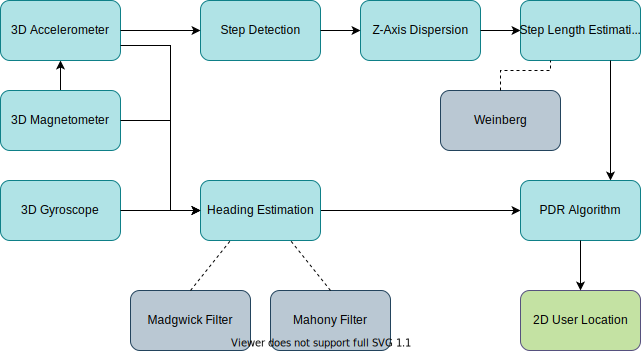
\includegraphics[scale=0.7]{Images/Experiments/pdr.pdf}
    \caption{PDR implementation architecture.}
     \label{fig:pdr}
\end{figure}

% Tag elementer fra filen geometry_based.tex fra 1.Problem_analysis til forklaring af PDR.

\subsection{Step Detection}

The general idea of step detection of a pedestrian with a smartphone is by measuring the accelerometer sensor and observe the increases and decreases in the acceleration pattern\cite{HybridPositioningPaper}. We have chosen to follow the algorithm proposed in \cite{peakdetection}. This is due to the fact that it is the only solution implementable for smartphones in a walking scenario.

The algorithm is based on the principle of dispersion, which is the extent to which a distribution is stretched or squeezed \cite{dispersion}. As seen in figure \textbf{\autoref{fig:pdr}}, the Z-axis dispersion is computed before the step detection. This step includes smoothening of the data to remove noise. This is included in the first step in \textbf{\autoref{fig:pdr}}, which is denoted by the number \textbf{1}.

For the step detection, which is \textbf{step 2} in \textbf{\autoref{fig:pdr}}, the algorithm will return a signal value if a new datapoint is a specific amount of deviations away from a moving mean. This amount of deviations is also called the z-score. The algorithm creates a separate moving mean and deviation, and signals can therefore not corrupt the threshold. The algorithm takes 3 inputs: \textit{lag}, \textit{threshold} and \textit{influence}. \textit{Lag} determines how much the input data is to be smoothened. Therefore, low lag values result in the algorithm being quicker at adapting to the input data. Since the input data for step detection vary a lot, the lag value will be low. The \textit{threshold} is the z-score at which the algorithm will return a signal. Lastly, the \textit{influence} is the impact of new signals on the mean and deviation. The influence can be between 0 and 1. If 0 is chosen as the influence, signals would be completely ignored for recalculation of a new threshold. This choice would assume stationarity, meaning that the statistical properties of a process, such as the mean, variance and the structure of the autocorrelation, do not change over time\cite{stationarity}. In our case, we are working with data from walking people in a shopping mall. Since random walking is not a stationary process, we will use a nonzero value\cite{peakdetection}. The \textit{threshold} value is set to 10, since this is the value we deemed as giving the best result for detecting steps for our data set by trial-and-error. The \textit{threshold} value is found by using a subset of the data provided by Indoor Location \& Navigation Competition from Kaggle that corresponds to a single step to evaluate when the algorithm signals a step. The \textit{lag} value is set to 2, and is found in the same way as the \textit{threshold} value.

\subsection{Step Length Estimation}

For step length estimation, there exists two methods: static and dynamic. The static method assumes a person is walking at a constant velocity, whereas the dynamic method makes use of an accelerator for dynamic estimation. Weinberg is one method for dynamic step length estimation. We have decided to use the Weinberg method due to its low error compared to other methods \cite{HybridPositioningPaper}. This is executed in \textbf{step 3} in \textbf{\autoref{fig:pdr}}.  

The Weinberg method is defined in \textbf{\autoref{eq:weinberg}}\cite{weinberg}.

\begin{equation} \label{eq:weinberg}
    l = k \sqrt[4]{a_{LPF, peak} - a_{LPF, valley}}
\end{equation}

In \textbf{\autoref{eq:weinberg}}, $k$ is a constant factor for unit conversion, $a_{LPF, peak}$ is the maximum acceleration in the z-axis and $a_{LPF, valley}$ is the minimum acceleration in the z-axis. The value $k = 0.5$ is used in \cite{HybridPositioningPaper}, and we also found that this value yielded the best result by error-and-trial.

\subsection{Heading Estimation}
\textbf{Step 4} is the heading estimation. The heading estimation is accomplished using \gls{ahrs}, which is a Python toolkit for estimation attitude containing several functions and utilities for the attitude estimations\cite{ahrs, FastAHRS}. According to \cite{MultisensorComparison}, Madgwick and Mahony perform best in comparison to other alternative algorithms, both of which are provided by \gls{ahrs}. But since Madgwick outperforms Mahony according to \cite{Ludwig2018ComparisonOA}, we have decided to experiment with Madgwick. The Extended Kalman Filter is also implemented because of it being one of the most widely used algorithms\cite{ahrs}. Both of these algorithms compute a set of quaternions, given a set of acceleration data and gyroscope data, from which a heading can be computed. Quaternions is a way of representing 3D rotations\cite{quaternion_math}.

\subsection{Position Estimation}

\textbf{Step 5} is the last step before achieving the 2D user location using equations \textbf{\autoref{eq:pdr_X}} and \textbf{\autoref{eq:pdr_Y}}.

\begin{equation} \label{eq:pdr_X}
    x_t = x_{t - 1} + l_t\cos(\theta_t)
\end{equation}

\begin{equation} \label{eq:pdr_Y}
    y_t = y_{t - 1} + l_t\sin(\theta_t)
\end{equation}

\textbf{\autoref{eq:pdr_X}} and \textbf{\autoref{eq:pdr_Y}} are the central equations to compute in order to estimate a location $(x_t, y_t)$ at time $t$, given a previous location $(x_{t - 1}, y_{t - 1})$, a step length $l_t$ and a heading $\theta_t$ in radian.
\section{Artificial Neural Network} \label{neuralnetwork}  
As mentioned in \textbf{\autoref{sec:scene_analysis}}, neural networks are organised into several layers, known as the \textit{input layer}, the \textit{hidden layer} and the \textit{output layer}, which is depicted in \textbf{\autoref{fig:ann}}. As the names suggest, the input layer takes the external data as input to the \gls{ann}, and the output layer outputs the computational results. A training phase is used to learn the datasets to assign weights to the neurons in the neural network based on error rates between the target output and actual output.\cite{SAIRAMYA2019253} To train an \gls{ann}, backpropagation and Gradient Descent is used to improve the performance of the model\cite{SAIRAMYA2019253, ann}.

\begin{figure}[H]
    \centering
    \includegraphics[scale=0.75]{Images/Experiments/ann_architecture.jpg}
    \caption{Four-layer neural network\cite{ann}.}
     \label{fig:ann}
\end{figure}

\subsection{Forward Propagation}
The phase of propagating an input vector through the network and getting an output is called \textit{forward propagation}. The \gls{ann} takes a vector as input which is passed to the input layer in \textbf{\autoref{fig:ann}}. The network can have one or several hidden layers after the input layer, each layer containing neurons. To get the output of a layer, the neurons or weights are multiplied by the input, and an activation function is applied to the result of the aforementioned computation.
%The number of neurons in the output layer equals the number of possible classifications. 
The output of the output layer will be the final prediction made by the \gls{ann}.\cite{ann} An activation function is applied in the layers of the \gls{ann} to introduce non-linearity. Without non-linear activation functions, several hidden layers do not make sense, as they do not add additional power compared to a single layer. Non-linear activation function also makes it possible to non-linearly map the input to the output, which is necessary for most real world application.%, which is also the reason for the \gls{ann} being called the universal function approximator. 
%to represent the value given by the node as preferred\cite{nnadl}. In this example, the node output is a probability. That is, a value between 0 and 1.
In the \gls{ann}, the output of the previous layer is given an input to the next layer, while the output of the output layer is the final prediction.%, known as \textit{feedforward} neural networks, where cycles are not allowed as in \textit{recurrent} neural networks.\cite{ann}

\subsection{Backpropagation}

The backpropagation algorithm is used for understanding how much the weights in a network contributes to the loss. When the network consists of multiple layers, the loss is a composition function of the weights in the earlier layers. The backpropagation algorithm is used to find the gradient of the composition function, which includes the magnitude and direction of the function. The algorithm uses the chain rule of differential calculus, which will compute the error gradient through summations of the local-gradient product over the different paths in the network from a node to the output. %This calculation can be done efficiently using dynamic programming, and the backpropagation algorithm is an application of dynamic programming. 

%The backpropagation includes two main phases: the forward phase and the backward phase.

The backpropagation includes two main steps: the forward pass to calculate loss and a backtracking step, which traverses backwards from the deeper layers to calculate the derivatives of the weights, with respect to the loss. The forward pass is calculated through forward propagation.
%In the forward phase, the training data is fed to the neural network, and a cascade of computations will happen throughout the layers using the current weights. The output from the training will be compared to the final predicted output, and the derivative of the loss function is computed. 
In the backwards phase, the goal is to use the chain rule to compute the gradient of the loss function, in respect to the different weights. The gradients can thereafter be used to update the weights, through gradient descent explained in the following section. In this way, we optimize the weights, so the neural network will gain knowledge of how to correctly map the inputs to the outputs of the neural network.\cite{nnadl}

\subsection{Gradient Descent}
Gradient Descent is an algorithm that updates weights and biases for neurons so that the output from the neural network approximates its prediction for all training inputs. The main idea is to find the weights and biases so that the cost, the \gls{mse}, is as small as possible. Minimising \gls{mse} makes it easier to change the weights and biases in order to improve performance compared to maximizing the number of correct detection outputs.\cite{ann}

We let \gls{mse} be a function defined as $C(v)$, where $v$ is a set of many variables. We can minimise the function $C(v)$ by finding where $C$, in the optimal case, achieves its global minimum. We find the minimum by computing derivatives of $C$, since this would tell us the slopes of the function, which in turn tells the minimum of $C$.\cite{ann}
\section{Long Short-Term Memory (LSTM)}

As mentioned in \textbf{\autoref{rnn1}}, there are different types of \gls{rnn}s, but the \gls{lstm} model is one of the most widely used in regards to \gls{ips}. We will therefore also use the \gls{lstm} structure for our experiment with \gls{rnn}.

In a recurrent network, the output from a previous step will be used as input for the next step. In an \gls{lstm} model, the nodes are recurrent, and they also include a cell state. This cell state is the working memory space which is used by the node, so the information can be stored and retrieved over multiple time steps. Therefore, in an \gls{lstm}, the input value, the previous output, and the cell state are all used in the calculations of the node. The results of this calculation are used to get an output value, but also to update the cell state. Besides from having parameters for defining how inputs should be used in the calculations, as in standard neural networks, the \gls{lstm}'s nodes also include gates. The gates are responsible for controlling the flow within the node, which especially includes determining how much of the saved information should be used in a given calculation. The gate parameters are made of weights and biases, and therefore, the input determines the behaviour. There are three types of gates in an \gls{lstm} network; the input gate, the forget gate and the output gate. The \gls{lstm} network can therefore be divided into three different parts, as shown in \textbf{\autoref{fig:lstm}}. 

\begin{figure}[H]
    \centering
    \includegraphics[scale=0.85]{Images/Experiments/lstm.pdf}
    \caption{Overview of an LSTM network.}
    \label{fig:lstm}
\end{figure}

In the first part of the \gls{lstm}, the network will try to determine whether the information from the previous timestamp is relevant or if it should be forgotten. In the second part, the cell will try to learn new information from the given input, and update the information. In the last step, the cell will pass the information that it has updated, from the current timestamp to the next timestamp. Besides from the cell state, the \gls{lstm} network also includes a hidden state, as known in standard \gls{rnn} networks. In \textbf{\autoref{fig:lstm}}, $H(t-1)$ denotes the hidden state of the previous timestamp, and $H(t)$ denotes the hidden state of the current timestamp. $C(t-1)$ and $C(t)$ denote the previous and current timestamps for the cell state, respectively. The cell state can be viewed as the long term memory of the system, and the hidden state can be seen as the short term memory. The information from the timestamps are used in the calculations in the different gates in the network.\cite{lstmVidhya}

The \gls{lstm} networks are less exposed to the vanishing gradient problem, mentioned in \textbf{\autoref{sec:vanishing_exploding_gradient_problem}}, but the exploding gradient problem can still be encountered. Another disadvantage of the \gls{lstm} is that they are very computational intensive.\cite{Yalcın2021}
\section{Gradient Boosting Decision Trees}
As also mentioned in the Problem Statement in \textbf{\autoref{sec:problemstatement}},
we wanted to experiment with Gradient Boosting Decision Trees and similar tree-based algorithms. %LightGBM is a framework for gradient boosting machine used with tree based learning algorithms. It is an open source Microsoft framework built in C++, and with \gls{api}s to integrate it into C\#, R or Python. The scikit-learn \gls{api} is implemented to supply different algorithms to apply to LightGBM. The default algorithm is the traditional \gls{gbdt} and scikit-learn also offers Random Forrest (RF) and others. All the algorithms used by LightGBM is based on machine learning from decision trees.\cite{LightGBM}

In the following section, decision trees will be elaborated, and thereafter what gradient boosting is and how it is applied to the decision tree structure.
%% HVORFOR ER LIGHTGBM GODT AT BRUGE???
%https://lightgbm.readthedocs.io/en/latest/Features.html

%GBDT
%https://lightgbm.readthedocs.io/en/latest/pythonapi/lightgbm.LGBMClassifier.html

\subsection{Decision Tree}
%HVAD ER DECISION TREES?
Decision tree is a basic model within supervised machine learning. This model can be represented as a tree, where each internal (non-leaf) node contains a condition that has children corresponding to the evaluation of the condition (most commonly either true or false). The leaf nodes correspond to a classification derived from traversing the decision tree top-down.\cite{AIBook}

%HVORDAN BYGGER VI DECISION TREES?
To construct a decision tree top-down as mentioned in \cite{AIBook}, the train set is used. The idea is to create the best possible split until reaching a classification, and thereby create a leaf node. It is preferred to create a split that will create pure subsets. To measure the purity of the subsets and determine the best split we use entropy, expected-entropy and information gain.

\begin{equation} \label{eq:entropy}
    H(X) = \sum_{x \in domain(X)} - P(X = x) * log_{2} (P(X = x))
\end{equation}

\textbf{\autoref{eq:entropy}} calculates the entropy or purity of a set \textit{X} by summing the calculated probability \textit{P(X = x)} of each classifications occurring in the set. Having an entropy at 0 means a pure subset, where having a subset with evenly distributed elements across the classes would result in an entropy of 1. 

After calculating the entropy of the training set, we want to calculate the entropy after splitting on a particular condition, which is called the expected-entropy. The expected entropy from splitting on condition \textit{Y} is thereby

\begin{equation} \label{eq:entropy1}
    H(X | Y = y) = \sum_{x \in domain(X)} - P(X = x | Y = y) * log_{2} P(X = x | Y = y)
\end{equation}

In \textbf{\autoref{eq:entropy1}}, we, similarly to calculating the entropy, calculate the expected-entropy. The overall calculation is the same, the only difference is that we now calculate the entropy given a particular condition \textit{Y}.

To determine the best split for the decision tree, we compare the original entropy of the training set to the expected-entropy for the different conditions. This comparison is called \textit{information gain}.

\begin{equation} \label{eq:information-gain}
    H(X) - H(X | Y)
\end{equation}

\textbf{\autoref{eq:information-gain}} calculates the information gain from splitting on condition $Y$ for set $X$. After calculating the information gain for all the different conditions, the best condition to split on is the one with highest information gain.

\subsection{Gradient Boosting}
Gradient boosting is a technique for gathering different simpler machine learning models into one. Often, it uses decision trees for this purpose. Using the decision trees as the simple model is called \textit{gradient boosting decision trees}. The model is similar to the random forest approach, where we ensemble several decision trees. Though, instead the idea is to repetitively use the decision tree model on a dataset including a potential loss. Thereby, the model will improve through gradient descent.\cite[Chapter~12]{GradientBoosting}

The aim of this process is to create more of a training phase, where it improves on a loss. This is done by assigning an equal weight to each observation in the dataset, and after evaluating the first tree, the weights are regulated. The weights of the observations that were difficult to classify will be increased for next decision tree.\cite[Chapter~12]{GradientBoosting}


%\subsection{Dropouts Meet Multiple Additive Regression Trees}
%As mentioned in \textbf{\autoref{sec:problemsmachinelearning}}, a huge issue for a lot of machine learning models is overfitting, as seen in \textbf{\autoref{sec:problemsmachinelearning}}. To combat the issue of overfitting for Gradient Boosting Decision Trees, \gls{dart} was developed to combat this issue. This algorithm was presented in a paper \cite{dart} by K. V. Rashmi and Ran Gilad-Bachrach, and applies the dropout technique to gradient boosting regression trees. This does not eliminate all overfitting, but reduces it to a certain extent.\cite{dart}

%Dropout is a technique used most commonly for neural networks to reduce overfitting, which is explained in \textbf{\autoref{sec:over_underfit}}. The technique is concerned with randomly dropping units with their connections from the neural network during the training phase. The purpose is to remove units before their start to overspecialise. The dropout technique, as presented in paper \cite{dropout}, has proved to increase performance of neural networks for supervised learning tasks, since it reduces overfitting.

%In each iteration, the different trees are assigned a probability to be dropped. At the bare minimum, at least a single tree is dropped in each iteration. In the paper \cite{dart}, they use the \textit{binomial-plus-one} technique to select which trees to drop and if no trees are selected, then one tree is randomly chosen to be dropped.


%\subsection{Level-wise vs. Leaf-wise construction}


%%% GBDT algorithm (the one used in the experiment)






%Parameters to implementation section
%https://lightgbm.readthedocs.io/en/latest/Parameters.html
\section{Problems with Machine Learning Models} \label{sec:problemsmachinelearning}
In this section, we will explore the disadvantages that can occur when working with machine learning models. Doing so will benefit to understand the problems and avoid mistakes.  

\subsection{Overfitting and Underfitting}\label{sec:over_underfit}

When working with machine learning, one of the biggest challenges is to create a model that is complex enough to solve hard problems, but not complex enough to misunderstand the concept. If the concept is too simple, we have a risk of underfitting. If the concept is too complex and only works for the training data, we have a risk of overfitting. In overfitting, the model is highly accurate on the training data, but would not generalise well, meaning that it would not perform well on unseen data. In underfitting, the model is often too simple, and will therefore struggle to identify the concept, and will therefore neither model the training data nor generalise to new data. It is therefore important to balance the complexity, so the model that is created produces the best generalisation.\cite{Hulten2018}

\subsection{Vanishing and Exploding Gradient Problem} \label{sec:vanishing_exploding_gradient_problem}

In \textbf{\autoref{neuralnetwork}}, the training of a neural network through gradient-based learning is described. When using gradients, there are different issues that can happen. The error gradient, which is used to update the weights in the network, can accumulate and result in a large gradient. Because of the large gradient, large updates to the weights will occur, and the network is in risk of being unstable. When the network is unstable, it may not learn from the training data, or result in Not A Number (NaN) weight values, which can not be updated. These large gradients are also referred to as exploding gradients.\cite{vanishingexploding}

Alternatively, we can also have derivatives that are too small, and the gradient will exponentially grow smaller when we propagate through the model, so we risk having a gradient that will vanish. This is referred to as the vanishing gradient problem.\cite{vanishingexploding}
\section{Hybrid} \label{sec:hybrid_theory}
The hybrid approach consists of estimating the position using a \gls{lfp} method and the \gls{pdr} algorithm. These algorithms of the hybrid solution can use each other to achieve more accurate position estimations. Furthermore, hybrid solutions tend to achieve better accuracy, as described in \textbf{\autoref{sec:hybrid}}. The approach can be implemented in three ways, each presented in the following sections.

It should be noted that the \gls{pdr} algorithm cannot estimate the floor level. Therefore, for all hybrid solutions, the floor is estimated by the \gls{lfp} method alone.

A class diagram is presented in \textbf{\autoref{fig:hybrid_class_diagram}}. Since we will be working with multiple types of machine learning algorithms, a class for each machine learning algorithm is contained within \textit{ML Wrapper}. \textit{ML Wrapper} and \textit{PDR} are used to make up the three types of hybrid solutions, mentioned in this section.

\begin{figure}[H]
    \centering
    \includegraphics[scale=1]{Images/Experiments/hybrid/HybridClassDiagram.pdf}
    \caption{Class diagram of hybrid solution.}
     \label{fig:hybrid_class_diagram}
\end{figure}

\subsection{Location Fingerprinting as Primary and Pedestrian Dead Reckoning as Support}
This approach makes use of \gls{lfp} for positioning, where the \gls{pdr} algorithm is only used as support for whenever the \gls{lfp} method is not given any available \gls{rssi} data as input in a given period time. 
It happens that the \gls{lfp} method cannot determine a position if there are no \gls{rssi} values for the ground truth position. This approach idea is depicted in \textbf{\autoref{fig:hybrid1}}. In this case, \gls{pdr} will take over from the last know position estimated by \gls{lfp}.

\begin{figure}[H]
    \centering
    \includegraphics[scale=0.85]{Images/Experiments/hybrid/approach1.pdf}
    \caption{Hybrid solution using \gls{lfp} as primary and \gls{pdr} as support, where Scene Analysis is offline when it is not able to make a position estimation given its input, and online when it is able to make a position estimation.}
     \label{fig:hybrid1}
\end{figure}

The performance of this hybrid option relies much on the performance of the \gls{lfp} method. \gls{pdr} will have no impact on the position estimations made by \gls{lfp}. However, as described, when there is no available \gls{rssi} data, \gls{pdr} will fill the missing position estimation. The less times it occurs that there is no available \gls{rssi} data, the more the performance of this hybrid option is alike the performance of the \gls{lfp} method alone. Described in \autoref{alg:mlpdr_hybrid} the hybrid approach is shown, where \gls{lfp} is as primary and \gls{pdr} as support. 

% previous_wifi_data_timestamp er sidste timestamp, hvor LFP blev brugt.
% time_limit is a timeout time within which we need an estimation from LFP. If not, use PDR.
\begin{algorithm}[H]
\SetAlgoLined
\SetKw{KwIn}{in}
\SetKwInOut{Input}{Input}
\Input{$timestamp$, $\text{imu\_data}$ and $\text{wifi\_data}$}
\KwResult{($\text{x}$, $\text{y}$, $\text{floor}$)}
  $\text{lfp\_position}$ = $\text{lfp\_estimate\_position}$($\text{wifi\_data}$)\;
  
  \If{$timestamp - \text{previous\_wifi\_data\_timestamp} > \text{time\_limit} \lor \text{is\_empty}$($\text{wifi\_data}$)}{
      Re-calibrate \gls{pdr} to previous position estimation if \textit{if-statement} evaluated to false in previous position estimation\;
      $\text{pdr\_position}$ = $\text{pdr\_estimate\_position}$($\text{imu\_data}$)\;
      
      return $\text{pdr\_position}$\;
  }
  
  return $\text{lfp\_position}$\;
 \caption{Hybrid approach using \gls{lfp} as primary and \gls{pdr} as support.}
 \label{alg:mlpdr_hybrid}
\end{algorithm}

\subsection{Pedestrian Dead Reckoning as Primary and Location Fingerprinting as Support}
In this approach, the \gls{pdr} algorithm has the main responsibility at estimating positions. Although, as described in \textbf{\autoref{sec:IMUPositioning}}, \gls{pdr} drifts the more measurements it is given as input. Therefore, we need the \gls{lfp} method to re-calibrate \gls{pdr} before it drifts too much. The threshold value, $t$, for the number of measurements given as input before \gls{pdr} is re-calibrated is adjusted by experiments. This approach is depicted in \textbf{\autoref{fig:hybrid2}}.

\begin{figure}[H]
    \centering
    \includegraphics[scale=0.85]{Images/Experiments/hybrid/approach2.pdf}
    \caption{Hybrid solution using \gls{pdr} as primary and \gls{lfp} as support, where $c$ is measurement count and $t$ is a threshold value for measurement count.}
     \label{fig:hybrid2}
\end{figure}

This option aims at improving the accuracy of the experiments of \gls{pdr} by re-calibrating \gls{pdr} at fixed points in time. The re-calibration is accomplished using the position estimation from \gls{lfp}, which makes the overall accuracy dependent on the accuracy of \gls{lfp} at re-calibration time.
Since the odds of a position estimation of the \gls{lfp} method is far off the ground truth is low, the \gls{pdr} method should have the optimal environment for estimating positions. And since the \gls{pdr} is re-calibrated at fixed points in time, \gls{pdr} should not drift too far away from the ground truth path. Therefore, this hybrid option should yield better results compared to the \gls{pdr} experiments because of its re-calibration, as we have noted during the \gls{pdr} experiments that it is accurate for fewer \gls{imu} measurements. Explaining this hybrid method, the \autoref{alg:pdrml_hybrid} is shown.


% recalibration_limit er en konstant for antallet af estimeringer før PDR skal gen-kalibreres.
\begin{algorithm}[H]
\SetAlgoLined
\SetKw{KwIn}{in}
\SetKwInOut{Input}{Input}
\Input{$timestamp$, $\text{imu\_data}$ and $\text{wifi\_data}$}
\KwResult{($\text{x}$, $\text{y}$, $\text{floor}$)}
  $\text{pdr\_position}$ = $\text{pdr\_estimate\_position}$($\text{imu\_data}$)\;
  $\text{lfp\_position}$ = $\text{lfp\_estimate\_position}$($\text{wifi\_data}$)\;
  $\text{measurement\_count}$ = $\text{measurement\_count} + 1$\;
  
  \If{$\text{measurement\_count} \geq \text{recalibration\_limit}$}{
      Re-calibrate \gls{pdr} to position estimation of \gls{lfp}\;
  }
  
  return ($\text{pdr\_position.get\_x}$(), $\text{pdr\_position.get\_y}$(), $\text{lfp\_position}.get\_floor$())\;
 \caption{Hybrid approach using \gls{pdr} as primary and \gls{lfp} as support.}
 \label{alg:pdrml_hybrid}
\end{algorithm}

\subsection{Average Between Location Fingerprinting and Pedestrian Dead Reckoning Outputs}
This approach makes use of both the \gls{lfp} and \gls{pdr} algorithms. This approach estimates the position by taking the average position estimation from \gls{lfp} and \gls{pdr}. The floor estimation is rounded to the closest integer. \gls{pdr} is re-calibrated after a number of measurements are given as input, where this number is estimated from experiments.

\begin{figure}[H]
    \centering
    \includegraphics[scale=0.85]{Images/Experiments/hybrid/approach3.pdf}
    \caption{Hybrid solution using the average position estimation from \gls{pdr} and \gls{lfp}where $c$ is measurement count and $t$ is a threshold value for measurement count.}
     \label{fig:hybrid3}
\end{figure}

It is possible that any of \gls{lfp} and \gls{pdr} estimate a position that is not close to the ground truth position at each position estimation. Therefore, if one of \gls{lfp} and \gls{pdr} is accurate and the other is not, the other will drag its position estimation away from the ground truth. This is a problem since \gls{pdr} is known to drift the more measurements it is given as input. However, it is also possible the \gls{lfp} method will make a position estimation that is far off the ground truth position.
Thereby, using the average between the position estimation of both \gls{lfp} and \gls{pdr} will decrease the impact of the inaccurate position estimation made by any of \gls{lfp} and \gls{pdr}. The approach of this method is explained in pseudo code in \autoref{alg:average_hybrid}.
However, the main motivation for this approach is that if both position estimation methods are accurate but each of them deviate a bit from the ground truth, then it is possible to achieve a better estimation by considering the estimations from both approaches.

% estimation_count er antallet af nuværende estimeringer.
% recalibration_limit er en konstant for antallet af estimeringer før PDR skal gen-kalibreres.
\begin{algorithm}[H]
\SetAlgoLined
\SetKw{KwIn}{in}
\SetKwInOut{Input}{Input}
\Input{$timestamp$, $\text{imu\_data}$ and $\text{wifi\_data}$}
\KwResult{($\text{x}$, $\text{y}$, $\text{floor}$)}
 $\text{lfp\_position}$ = $\text{lfp\_estimate\_position}$($\text{wifi\_data}$)\;
 $\text{pdr\_position}$ = $\text{pdr\_estimate\_position}$($\text{imu\_data}$)\;
 $\text{avg\_x}$ = $\text{pdr\_position}.get\_x$()\;
 $\text{avg\_y}$ = $\text{pdr\_position}.get\_y$()\;
 
 \If{$\text{lfp\_position}$ $\neq$ $\text{null}$}{
     $\text{avg\_x}$ = ($\text{avg\_x}$ + $\text{lfp\_position}.get\_x$()) / 2\;
     $\text{avg\_x}$ = ($\text{avg\_y}$ + $\text{lfp\_position}.get\_y$()) / 2\;
     
     \If{$\text{estimation\_count > recalibration\_limit}$}{
         Re-calibrate \gls{pdr} to position estimation of \gls{lfp}\;
     }
     
 return ($\text{avg\_x}$, $\text{avg\_x}$, $\text{lfp\_position}.get\_floor$())
 }
 \caption{Hybrid approach using average between \gls{lfp} and \gls{pdr} for position estimation.}
 \label{alg:average_hybrid}
\end{algorithm}

%\subsection{Hybrid Approach of Choice}
\todowarning{Kig på dette senere. Der er opgave på det på Github}
%Since we know that \gls{pdr} drifts and will drag \gls{lfp} away if \gls{lfp} estimates a position that is accurate, and that re-calibration of \gls{pdr} can lead to even more inaccurate position estimations if \gls{lfp} is inaccurate at re-calibration time, we have decided to prioritise the implementation of the first option, where \gls{lfp} is the primary and \gls{pdr} the supporter. This choice is because of the accuracy of the \gls{lfp} method alone and because \gls{pdr} can be used whenever \gls{lfp} cannot, as previously described, to make up for the missing position estimations by \gls{lfp}.

% Måske det ikke giver mening at teste med ML som primary og PDR som support, da det kan undersøges i datasættet, om der er udfalg, hvor PDR vil tage over. Derudover vil PDR alligevel ikke rigtig komme igang. Hvis ML ikke kan lave estimeringer, vil det alligevel være i så kort tid, at PDR ikke kan nå at lave nogel estimeringer, da det tager en del målinger for at udgøre et skridt.

\chapter{Experiments}
\textit{After processing the data, it is now possible to create different experiments for predicting locations. Before starting on the different experiments, we wanted to create a general pattern and flow of the experiments, which will be covered first. Thereafter, the different experiments and their evaluation will be covered.}
\section{Task Definition}
Thoughout this chapter, we will be conducting experiments with the purpose of solving the problem statement. To help in the process of conducting the experiments, we need to reify the objectives of the experiments. To this end we can define subtasks with respect to the problem statement, which we can use as goals for the experiments. The problem, which we are working on, is to identify the position in an indoor environment given data collected by a smart phone. The position is specified as a X-coordinate, Y-coordinate and floor level. To this end, we can define subtasks for identifying each of the specifications:
\begin{center}
    \textbf{Estimate the X-coordinate}
\end{center}
\vspace{-0.8cm}
\begin{center}
    \textbf{Estimate the Y-coordinate}
\end{center}
\vspace{-0.8cm}
\begin{center}
    \textbf{Estimate the floor level}
\end{center}
Even though the subtasks are defined as three separate tasks, it might be ideal to combine them when conducting an experiment. E.g. it might the case that a relationship between the X- and Y-coordinate exists or between all of the subtasks. This might lead to a model which solves more than one subtasks being superior to a model which is specialised only towards one of the subtasks. 

\section{Experiment Flow}
To start off the process, we wanted to create an overall architecture for the experimental process similar to the one shown in \textbf{\autoref{fig:DataArchitecture}}. The data is being prepared for each individual experiment in the \textit{Data Pipeline} phase before reaching the \textit{Experiments} phase.

\begin{figure}[H]
    \centering
    \includegraphics[scale=.34]{Images/Experiments/ExperimentFlow.png}
    \caption{The overall architecture with added evaluation.}
    \label{fig:experimentflow}
\end{figure}

As seen on \textbf{\autoref{fig:experimentflow}}, we have expanded on the \textit{Experiments} component to also interact with the \textit{Evaluation} component. This new component takes the ground truth data and compares it to estimations from the experiment. For this purpose, the \textit{Data Pipeline} component now passes the data to the \textit{Experiments} component and also the ground truth data to the \textit{Evaluation} component. The \textit{Evaluation} component now compares the result of the experiment to the ground truth and thereby evaluates the experiment. These results can be reflected on, which might lead to new experiments, which is indicated by the interaction from the \textit{Evaluation} component to the \textit{Experiment} component.

\subsection{Experiments}
The \textit{Experiments} component in \textbf{\autoref{fig:experimentflow}} denotes the implementation and use of the positioning methods, mentioned in \textbf{\autoref{sec:problemstatement}}, which we would need to test. The different experiments will include LightGBM, \gls{ann}, \gls{hmm}, k-NN and \gls{imu}-based methods. Each experiment takes the input data from the \textit{Data Pipeline} phase. As mentioned in \textbf{\autoref{sec:datapipeline}}, this component is concerned with processing the data for the specific positioning method in the experiment. After receiving the data from the \textit{Data Pipeline} component, the implementation of the experiment will be executed to achieve estimations of the indoor locations. The estimations from these experiments will then be forwarded to the \textit{Evaluation} phase to determine the performance of the model.
%Elaborate the Experiment part of the design
%Generelt om hvad et eksperiment er + hvilke eksperimenter vi prøver af
%Kontekst til de andre dele (data pipeline + evaluation)
%Input og output til experiments
%

\subsection{K-Fold Cross Validation}
K-Fold Cross Validation is a statistical method used to evaluate machine learning models on a limited data sample. K-Fold Cross Validation enables the option to use the entire dataset for training and testing the machine learning models compared to techniques like splitting the dataset into training, validation and test sets, and using these dataset to train, validate, and evaluate the model. It is also a useful way to test multiple machine learning methods to evaluate which of the methods works best for the data. 
The idea with K-Fold Cross Validation is to split the dataset into equally sized $K$ groups and use one of the groups as a validator to evaluate the performance of the models. This process is executed $K$ times where the group being the validator is shifted between the groups.\cite{kfold}

\begin{figure}[h]
    \centering
    \includegraphics[scale = 0.7]{Images/Experiments/k-fold.pdf}
    \caption{Process on K-Fold Cross Validation}
    \label{fig:kfold}
\end{figure}

As seen on \autoref{fig:kfold}, the dataset is split into $K$ groups, where $K-1$ groups will be used to train a machine learning model. The model will then be evaluated on the validator partition based on metrics like the accuracy. Afterwards, the validator will be shifted to another group and the machine model will be trained and get a score. This will be executed until all groups have been the validator. Each model will be discarded after the evaluation such that a new model is trained and evaluated in each iteration. The scores would then be summarized and will be the score for said model.  
This procedure can be used on multiple models to compare the scores and determine the better model.

The value of $K$ can be configured and a poorly chosen $K$ can result in poor performance. According to \cite{kfold_configk}, the choice of the value for $K$ is usually 10 since the value have shown an empirical test error rate which experienced best performance.    

\subsection{Evaluation}
To evaluate the different experiments, which is depicted as the \textit{Evaluation} component in \textbf{\autoref{fig:experimentflow}}, we have decided to implement a generic Evaluator, which can be used to evaluate the different models/algorithms in terms of different performance metrics.
This Evaluator should evaluate the result with regards to \textbf{\autoref{eq:rmse}} on X-, Y- and floor-coordinate separately, where $v'$ denotes the ground truth coordinate value and $v$ denotes the estimated coordinate value. Additionally, the Evaluator should also calculate the position error with regards to each estimation made by the algorithm/model.

\begin{equation}
    \text{\gls{rmse}} = \frac{1}{n} \sum_{i = 1}^{n} \sqrt{(v_{i}' - v_i)^2}
    \label{eq:rmse}
\end{equation}

The Evaluator takes the position estimations from the \textit{Experiments} phase and the ground truth data from the \textit{Feature Engineering} component as input. From this, it is possible to calculate the \gls{rmse} of each position coordinate and the position error for each individual estimation. All of the performance metrics as well as the input to the Evaluator should be recorded to a file dedicated for the evaluation output. The execution of the generic evaluation class should be integrated into each experiment, where it is possible to work with the results and maybe add additional evaluations.

It should be noted that the \gls{pdr} algorithm will be evaluated differently since it is only able to estimate positions on a 2-dimensional level. \gls{pdr} will be still be evaluated by each of its position estimations, but will also use \textbf{\autoref{eq:MeanPositionError}} defined in \textbf{\autoref{sec:kaggleComp}} for its overall performance on each path.

% NOTER: 
% - Eksperimenter evalueres af single, central evaluator.
% Evaluate waypoints individually with position error
% Evaluator outputter resultater for hver enkelt waypoint.
%   Output indeholder ground truth, estimering, og position error for hvert enkelt prediction.
%   Output konkluderer med mean position error.
% Evaluatator tager ground truth data og estimeringer som input og udregner de nødvendige evalueringer og skriver dem i sidste ende til filer.
% Eksekvering af evaluator skal ske som en integreret del af hvert enkelt eksperiment.
% Evaluator skal generere output i 'output' folder.

\subsection{Frameworks and Libraries}
For implementing the different experiments and the generic evaluation class, we have decided to use the programming language Python for consistency with the development of the data handling. Furthermore, most of the methods or techniques, which we would like to implement and test, are supported in Python in terms of frameworks and libraries, making it the ideal programming language for this.

To implement these experiments, we will be using different frameworks and libraries. For some of the experiments, we have decided to use TensorFlow, which is an open-source machine learning platform, which contains implementations of the different machine learning algorithms that we want to experiment with. \cite{TensorFlow}

We also use the Light Gradient Boosting Machine (LightGBM)  framework for some experiments. It is a machine learning framework and is designed to use tree-based learning for higher efficiency and better distribution of workload. This framework also contains an implementation of k-fold cross validation.\cite{LightGBM}

LightGBM utilises the library sci-kit learn to perform the calculations for the models. Sci-kit learn consists of several different algorithms which are used by LightGBM. In this way LightGBM act as a structuring framework to help utilise the functionality of sci-kit learn. \cite{scikit}

As mentioned in \textbf{\autoref{sec:pdr}}, we will use the \gls{ahrs} toolkit for the heading estimation in the PDR algorithm, which is a Python toolkit for attitude estimations. More specifically, we will use the Madgwick and the Extended Kalman Filter from \gls{ahrs}.\cite{ahrs}


% Vi bruger Python til det hele udover til wrapper til libs.
% TensorFlow (Neural network, HMM, knn og RNN)
% LightGBM


%\subsection{Coding Standard}
% - Kommentar på alle metoder/funktioner/procedurer.
%   - Kommentarer skal komme den sidste linje før deklaration.
% - Snake-case til symbol deklarationer.
% - 
\section{Pedestrian Dead Reckoning} \label{sec:IMUPositioning_eval}
This section describes the evaluation of the \gls{pdr} algorithm using Madgwick orientation filter and Extended Kalman Filter for heading estimation.

%We will present a cumulative distribution graph of the evaluation results of the two experiments, one for each heading estimation filter. 
%Furthermore, 
An average positioning error has been computed of all positioning errors, but it is important to note that this value is highly affected by the length of each path in the evaluation. This is because the positioning error is accumulative for \gls{pdr}, as mentioned in \textbf{\autoref{sec:IMUPositioning}}. Therefore, the shorter a path in the evaluation is, the more the average positioning error is dragged towards a lower value, and therefore, this value does not truly represent the performance of a \gls{pdr} implementation of one heading estimation filter. However, the average positioning error can be used to compare the different \gls{pdr} implementations with the two different heading estimation filters, since both are evaluated on the same data and paths. Furthermore, the position errors of both filters for selected paths have been shown and evaluated on, as seen in \textbf{\autoref{PDR:results}}. The most remarkable diagrams are the diagrams shown in \textbf{\autoref{fig:pdr_performance}}. As it can be seen from the experiment results in \textbf{\autoref{PDR:results}}, the \gls{pdr} algorithm using Madgwick Filter for heading estimations performs best, since its positioning error is lower than the \gls{pdr} algorithm using Extended Kalman Filter for heading estimation. Furthermore, as explained in \textbf{\autoref{sec:IMUPositioning}}, the \gls{pdr} algorithm drifts the longer the path is, resulting in higher positioning errors per measurement. It is noticeable that the \gls{pdr} algorithm improves its estimations per measurement in \textbf{\autoref{fig:pdr_performance}(c)}. The reason for this might be that the \gls{pdr} algorithm makes three wrong heading estimations at measurement 748, 1654 and 2089 that turns the pedestrian toward the ground truth path.

The mean positioning errors across all paths for Madgwick and Extended Kalman Filter are 34.78 meters and 43.83 meters, respectively.

\begin{figure}[H]
\centering
\SetFigLayout{2}{2}
  \subfigure[]{\includegraphics{Images/Experiments/pdr/pdr1.png}}
  \hfill
  \subfigure[]{\includegraphics{Images/Experiments/pdr/pdr10.png}}
  \hfill
  \subfigure[]{\includegraphics{Images/Experiments/pdr/pdr12.png}}
  \hfill
  \subfigure[]{\includegraphics{Images/Experiments/pdr/pdr15.png}}
  \hfill
  \caption{\gls{pdr} performance using Madgwick Filter and Extended Kalman Filter for heading estimation.}
  \label{fig:pdr_performance}
\end{figure}

Furthermore, we have analysed the timestamps between the measurements. The longer the \gls{pdr} algorithm has to wait till next measurement, the more likely the position estimation is to be inaccurate. On \textbf{\autoref{fig:pdr_boxplot}} is seen a diagram that depicts the minimum, maximum and median variance in measurement timestamps.

\begin{figure}[H]
    \centering
    \includegraphics[scale = 0.55]{Images/Experiments/pdr/boxplot.png}
    \caption{Variance in measurement timestamps in seconds. The lowest line is the minimum timestamp difference, the middle line is the median and the highest line is the maximum.}
    \label{fig:pdr_boxplot}
\end{figure}

As seen on \textbf{\autoref{fig:pdr_boxplot}}, the is quite a difference from the median to the maximum measurement timestamp difference. The middle line consists of three lines; the median, 1st quartile and 3rd quartile. Because these three lines are so close to each other, it means that only a few of the measurement timestamps differ more than 0.02 from the previous measurement timestamp. These few measurement timestamps that differ more than 0.02 may be the reason to some of the major wrong heading estimations, since the heading estimation is based on receiving data with a given frequency. Therefore, these few measurement timestamps will temporarily decrease the expected frequency.

As seen on \textbf{\autoref{fig:pdr_cdf}}, it is clear that the Madgwick Filter implementation outperforms the Extended Kalman Filter implementation by their \gls{cdf}, since it can be seen in \textbf{\autoref{fig:pdr_cdf}(b)} that positioning errors using Extended Kalman Filter reach higher position errors values with a maximum of 565.02 meters compared to using Madgwick Filter with a maximum positioning error of 400.40 meters, seen in \textbf{\autoref{fig:pdr_cdf}(a)}. Furthermore, the positive slope of \gls{cdf} decreases at positioning error around 50 meters for \textbf{\autoref{fig:pdr_cdf}(a)}, whereas this does not happen until at around 100 meters for \textbf{\autoref{fig:pdr_cdf}(b)}. This generally means that the Extended Kalman Filter implementation outputs position estimations that are further off the ground truth position compared to the Madgwick Filter implementation.

\begin{figure}[H]
\centering
  \SetFigLayout{1}{2}
  \subfigure[]{\includegraphics{Images/Experiments/pdr/cdf_madgwick.png}}
  \hfill
  \subfigure[]{\includegraphics{Images/Experiments/pdr/cdf_kalman.png}}
  \caption{\gls{cdf} for Madgwick Filter implementation (a) and Extended Kalman Filter implementation (b).}
  \label{fig:pdr_cdf}
\end{figure}

Because the \gls{pdr} algorithm performs best using Madgwick Filter, this will be our choice of heading estimation filter for the algorithm.
\section{Artificial Neural Network} 
In this section, we will describe and reflect upon the result of the \gls{ann} experiments conducted in this project. We will also evaluate the performance of the \gls{ann} architecture proposed by \cite{} as we mentioned in \textbf{\autoref{}}. For the evaluation of the 
 
\subsection{Initial Model}
Initially, we have tested a variety of models, and we end up with the following initial model, which comparatively speaking performs well.
For our initial model, we have tested a model with the following specification:

\begin{table}[H]
    \centering
    \caption{Model Specification for initial \gls{ann} experiment.}
    \begin{tabular}{m{0.3\textwidth}m{0.2\textwidth} m{0.2\textwidth}}
        \hline
        \multicolumn{1}{c}{\textbf{Description}} & \multicolumn{1}{c}{\textbf{Neurons}} & \multicolumn{1}{c}{\textbf{Activation}}\\
        \hline
        
        Input Layer         &   \multicolumn{1}{c}{$N$} & \multicolumn{1}{c}{None}        \\
        1. Hidden Layer     &   \multicolumn{1}{c}{$\frac{1}{4}N$}  & \multicolumn{1}{c}{ReLU}     \\
        2. Hidden Layer     &   \multicolumn{1}{c}{$\frac{1}{2}N$}  & \multicolumn{1}{c}{ReLU}     \\
        Output Layer     &   \multicolumn{1}{c}{$1$}  & \multicolumn{1}{c}{None}     \\
        \hline
    \end{tabular}
    \label{tab:NN01}
\end{table}

% \begin{itemize}
%     \item A hidden layer with neurons amounting to half of the input neurons and relu activation function
%     \item A hidden layer with neurons amounting to $1/4$ of the input neurons and relu activation function
%     \item A hidden layer with neurons amounting to half of the input neurons and relu activation function
%     \item A output layer with one neuron
%     \item As gradient descent, Adam has been used with a learning rate of 0.01 in a batch size of 32.
% \end{itemize}
Models with the specification mentioned in \textbf{\autoref{tab:NN01}} have been trained for each site and for each X, Y, and floor. We have decided to implement models for X, Y, and floor separately as we believe that a more specific model will have better performance as it does not need to focus on more than one prediction. The models have been trained with the optimiser Adam, which is a variation of stochastic gradient descent, and in batches of size 32. The models have been trained for 100 epochs, but with early stopping with patience of 10 epoch in the validation loss. This means that if the validation loss does not improve in 10 epochs, the training of the model will end.

\subsubsection{Results of First Test}
The results of this model specification varies depending on the whether the prediction is X,Y or floor. We will evaluate each of them respectively. For the Y-values, when looking at the development of the training and validation loss, we can see that for most of the cases the initial loss is high. This can be seen on (a) on \textbf{\autoref{fig:NN01}}. Even when investigating the training after the initial training period, we can still see that the model struggles to find the optimal state and the final loss furthermore also seems to be quite high. This is indicated on (b) on \textbf{\autoref{fig:NN01}}. Furthermore, the mean of the \gls{mse}s for all sites for the training data and validation data are at 9372 and 2407.32, respectively. This further illustrates the issue of not finding an optima. 

\begin{figure}[H]
\centering
  \SetFigLayout{1}{2}
  \subfigure[]{\includegraphics{Images/Experiments/NN/1.initial/all/5d27075f03f801723c2e360f_y.png}
  }
  \hfill
  \subfigure[]{\includegraphics{Images/Experiments/NN/1.initial/after20/5d27075f03f801723c2e360f_y.png}}
  \caption{The performance for a site.}
  \label{fig:NN01}
\end{figure}
% \begin{figure}[h]
%     \centering
%     \includegraphics[scale=0.5]{Images/Experiments/NN/expr01/5da138764db8ce0c98bcaa46_y(0).png}
%     \caption{Training with all epochs}
%     \label{fig:NN_01}
% \end{figure}
% \begin{figure}[h]
%     \centering
%     \includegraphics[scale=0.5]{Images/Experiments/NN/expr01/5da138764db8ce0c98bcaa46_y.png}
%     \caption{Training with epoch 2 and onward}
%     \label{fig:NN_02}
% \end{figure}
As with Y, we notice the same tendencies with results for the X predictions. The result of the same site as in \textbf{\autoref{fig:NN01}} is shown for the result for X estimations in \textbf{\autoref{fig:NN01_x}}. The mean of the \gls{mse}s for the sites for the X estimations are at 4967 and 3077 for the training and validation datasets, respectively.
\begin{figure}[H]
    \centering
    \includegraphics[scale=0.4]{Images/Experiments/NN/1.initial/5d27075f03f801723c2e360f_x.png}
    \caption{Results for site 5d27075f03f801723c2e360f for X estimations.}
    \label{fig:NN01_x}
\end{figure}
Among the estimations, we observe the worst behaviour for the floor estimations, when considering the mean of \gls{mse}s, which are at $166586.22$ and $8538.34$ for the training and validation data, respectively. However, for most of the sites for the floor predictions, we achieve good results, but the overall mean is dragged up due to a few extreme results. One of the good results is displayed in \textbf{\autoref{fig:NN01_floor}}.
\begin{figure}[H]
    \centering
    \includegraphics[scale=0.4]{Images/Experiments/NN/1.initial/5d27075f03f801723c2e360f_floor.png}
    \caption{Results for site 5d27075f03f801723c2e360f for floor estimations.}
    \label{fig:NN01_floor}
\end{figure}

The overall issue with struggling to find the optima, which we observe especially for the X and Y estimations, can have a number of reasons. The reasoning for this, which we think is most likely, might be due to a high learning rate or due to the model being unable to properly localise the optimum in the raw dataset. To this end, we will try to decrease the learning rate in one experiment and try training with the normalised dataset in another experiment.


\subsubsection{Results of Second Test}
After conducting the experiment with an adjusted learning rate of 0.001, we achieve better results compared to the initial experiment for all the models. This is deemed from the mean of \gls{mse}s on both training and validation dataset. 

%The results for the site, which we have shown for the earlier experiment, is shown here. 
%In the initial experiment, we end up with a loss around 1600, while in with the adjusted learning rate we achieve a loss around 50. This is further illustrated by the mean of the \gls{mse}s on the training and validation dataset, which is 1590 and 2191 for the initial experiment, while it becomes 516 and 475 for the second experiment for the training and validation \gls{mse}s, respectively.
% \begin{figure}[H]
% \centering
%   \SetFigLayout{1}{2}
%   \subfigure[]{\includegraphics{Images/Experiments/NN/2.adjustedLR/5d27075f03f801723c2e360f_y_all.png}
%   }
%   \hfill
%   \subfigure[]{\includegraphics{Images/Experiments/NN/2.adjustedLR/5d27075f03f801723c2e360f_y_34.png}
%   }
%   \caption{The performance for a site.}
%   \label{fig:NN02}
% \end{figure}
\begin{figure}[H]
\centering
  \SetFigLayout{1}{2}
  \subfigure[]{\includegraphics{Images/Experiments/NN/1.initial/exp2_y_5d27075f03f801723c2e360f.png}
  }
  \hfill
  \subfigure[]{\includegraphics{Images/Experiments/NN/1.initial/exp2_x_5d27075f03f801723c2e360f.png}}
  \caption{Results for site 5d27075f03f801723c2e360f for y estimations (a) and x estimations (b).}
  \label{fig:exp2}
\end{figure}

\textbf{\autoref{fig:exp2}} displays the result of the X and Y estimations. For the X estimations, the mean of \gls{mse}s are 669 \& 2298.73 for training and validation, respectively. This is still a quite huge gap between the training and validation loss. For the Y estimations, we achieve a mean of \gls{mse}s of 1159 for training and 230.59 for validation.  Lastly for the Floor model, we achieve 8891 for training dataset and 533.03 for validation dataset. We see an improvement in comparison to the initial test, but overall the performance still does not seem ideal.

%\begin{figure}[H]
   % \centering
   % \includegraphics[scale=0.5]{Images/Experiments/NN/1.initial/e%xp2_floor_5d27075f03f801723c2e360f.png}
   % \caption{Results for site 5d27075f03f801723c2e360f for floor %estimations.}
   % \label{fig:exp2_floor}
%\end{figure}

\subsubsection{Results of Third Test}
We have also conducted the experiment with a normalised dataset. The data is normalised through Min-Max Normalisation, which is used to scale features as mentioned in \autoref{sec:minmaxnormalisation}. Applying this to the \gls{ann} model should lead to a decrease in the loss and an increase in the performance of the model.

\begin{figure}[H]
\centering
  \SetFigLayout{1}{2}
  \subfigure[]{\includegraphics{Images/Experiments/NN/1.initial/exp3_y_5d27075f03f801723c2e360f.png}
  }
  \hfill
  \subfigure[]{\includegraphics{Images/Experiments/NN/1.initial/exp3_x_5d27075f03f801723c2e360f.png}}
  \caption{Results for site 5d27075f03f801723c2e360f for y estimations (a) and x estimations (b).}
  \label{fig:exp3}
\end{figure}

After using the normalised data instead, the mean of \gls{mse}s dropped significantly, which can be seen on \textbf{\autoref{fig:exp3}}. The \textit{X} model has dropped from a mean of \gls{mse}s from 4967 on the initial model to 10.41 on the training data. The \textit{Y} model has decreased from a mean of \gls{mse}s from 9372 on the initial model to 8.98 on the training data. As can be seen from the graphs, the validation loss is quite high compared to the training loss, which is not an issue of same degree with adjusting the learning rate.

%\begin{figure}[H]
    %\centering
    %\includegraphics[scale=0.5]{Images/Experiments/NN/1.initial/exp3_floor_5d27075f03f801723c2e360f.png}
    %\caption{Results for site 5d27075f03f801723c2e360f for floor estimations.}
    %\label{fig:exp3_floor}
%\end{figure}
%Here we get a mean on \gls{mse}s for training and validation of 5.6 and 14.9, respectively. The loss is significantly less compared to the previous experiments. 

The most significant change is in the \textit{Floor} model, which decreases the mean of \gls{mse}s to 0.034 for the training dataset and 0.0334 for validation dataset. This proves the assumption about the data making the model unable to properly localise the optimum. Since both reducing the learning rate and using the normalised data combined might lead to even better results. 


\subsection{Result of Fourth Test}
We have also tried a combination of min-max normalised dataset as well as less learning rate, which seems to give good performance. 

\begin{figure}[H]
\centering
  \SetFigLayout{1}{2}
  \subfigure[]{\includegraphics{Images/Experiments/NN/1.initial/exp4_y_5d27075f03f801723c2e360f.png}
  }
  \hfill
  \subfigure[]{\includegraphics{Images/Experiments/NN/1.initial/exp4_x_5d27075f03f801723c2e360f.png}}
  \caption{Results for site 5d27075f03f801723c2e360f for y estimations (a) and x estimations (b).}
  \label{fig:exp4}
\end{figure}

This for the X and Y model resulted in losses as displayed in \textbf{\autoref{fig:exp3}}, which displays quite a decrease in loss compared to the prior experiments. The graphs seem to perform a bit worse on the validation dataset than for the training dataset, which could be due to slight overfitting.

\begin{figure}[H]
    \centering
    \includegraphics[scale=0.5]{Images/Experiments/NN/1.initial/exp4_floor_5d27075f03f801723c2e360f.png}
    \caption{Results for site 5d27075f03f801723c2e360f for floor estimations.}
    \label{fig:exp4_floor}
\end{figure}

For the \textit{Floor} model, the performance has increased severely since the initial model. The final mean of \gls{mse}s for the training set is 0.0019 and for the validation set is 0.0027.

%We have also calculated the mean of the \gls{mse} for training data and test data is 4.4 and 12.2, respectively. The result, which we achieve for the normalised and less learning rate, seem to perform the best.




\subsubsection{Evaluation of Initial Model}
To evaluate the initial model, we use the \gls{mse}. After determining the most optimal hyper parameters, the k for k-fold should be determined. On \textbf{\autoref{tab:NN_train_initial_results}} and \textbf{\autoref{tab:NN_val_initial_results}}, we see the results for the training data and validation data for the three models (\textit{X}, \textit{Y} and \textit{Floor}). Each model is decribed by the best of k \gls{mse}s, the mean of the \gls{mse}s and the worst of k \gls{mse}s.

\begin{table}[H]
    \centering
    \caption{Results of the training dataset for initial \gls{ann} models, where \textbf{B} stands for the best of k \gls{mse}s, while \textbf{M} stands for the mean of the \gls{mse}s, and \textbf{W} stands for the worst.}
    \begin{adjustbox}{max width=\textwidth}
    \begin{tabular}{m{0.15\textwidth}@{\extracolsep{0.1cm}} m{0.05\textwidth}@{\extracolsep{0pt}} m{0.05\textwidth} m{0.05\textwidth} @{\extracolsep{0.1cm}} m{0.05\textwidth}
    @{\extracolsep{0pt}}
    m{0.05\textwidth} m{0.05\textwidth} @{\extracolsep{0.1cm}} m{0.05\textwidth}@{\extracolsep{0pt}} m{0.05\textwidth} m{0.05\textwidth}}
        \hline
         \multirow{2}{*}{\centering
         \textbf{Description}} & \multicolumn{3}{c}{\textbf{X}} & \multicolumn{3}{c}{\textbf{Y}}& \multicolumn{3}{c}{\textbf{Floor}}\\
         \cline{2-10}
         & \multicolumn{1}{c}{\textbf{B}} & \multicolumn{1}{c}{\textbf{M}}& \multicolumn{1}{c}{\textbf{W}}& \multicolumn{1}{c}{\textbf{B}}& \multicolumn{1}{c}{\textbf{M}}& \multicolumn{1}{c}{\textbf{W}}& \multicolumn{1}{c}{\textbf{B}}& \multicolumn{1}{c}{\textbf{M}}& \multicolumn{1}{c}{\textbf{W}}\\
        \hline\\
        Initial Model & \multicolumn{1}{c}{1073} & \multicolumn{1}{c}{4967} & \multicolumn{1}{c}{$3.1\cdot10^{4}$} & \multicolumn{1}{c}{731} & \multicolumn{1}{c}{9372} & \multicolumn{1}{c}{$7.3\cdot10^{4}$} & \multicolumn{1}{c}{2.67} & \multicolumn{1}{c}{$1.6\cdot10^{5}$} & \multicolumn{1}{c}{$1.6\cdot10^{6}$}
        \\\\
        %\\\hline\\
        Adjusted LR & \multicolumn{1}{c}{72.38} & \multicolumn{1}{c}{669} & \multicolumn{1}{c}{5414} & \multicolumn{1}{c}{77.30} & \multicolumn{1}{c}{1159} & \multicolumn{1}{c}{807} & \multicolumn{1}{c}{1.25} & \multicolumn{1}{c}{8891} & \multicolumn{1}{c}{79966}
        \\\\
        %\\\hline\\
        Normalised Data & \multicolumn{1}{c}{8.03} & \multicolumn{1}{c}{10.41} & \multicolumn{1}{c}{15.89} & \multicolumn{1}{c}{6.75} & \multicolumn{1}{c}{8.98} & \multicolumn{1}{c}{11.63} & \multicolumn{1}{c}{$9.3\cdot 10^{-4}$} & \multicolumn{1}{c}{0.034} & \multicolumn{1}{c}{0.25}
        \\\\
        %\\\hline\\
        Adjusted LR \& Normalised Data & \multicolumn{1}{c}{5.41} & \multicolumn{1}{c}{7.45} & \multicolumn{1}{c}{9.40} & \multicolumn{1}{c}{4.87} & \multicolumn{1}{c}{6.47} & \multicolumn{1}{c}{7.25} & \multicolumn{1}{c}{$9.5\cdot 10^{-4}$} & \multicolumn{1}{c}{0.0019} & \multicolumn{1}{c}{0.0047}
        \\\hline
    \end{tabular}
    \end{adjustbox}
    \label{tab:NN_train_initial_results}
\end{table}

\textbf{\autoref{tab:NN_train_initial_results}} displays the \gls{mse}s for the training dataset. The first row displays information about the initial model before adjusting the learning rate and using the normalised data. Especially, using the normalised data decreases the \gls{mse}s for all the models with both best and worst k \gls{mse}s. Last row describes the model after both adjusting the learning rate and using the normalised data. This model clearly decreases the \gls{mse}s compared to the previous models. The \textit{X} model has decreased from a mean of \gls{mse}s of 4967 to 7.45, and the \textit{Y} model has decreased from a mean of \gls{mse}s of 9372 to 6.47. The model for predicting floors has decreased extremely from a mean of \gls{mse}s of 160000 to 0.0019.

\begin{table}[H]
    \centering
    \caption{Results of the validation dataset for initial \gls{ann} models, where \textbf{B} stands for the best of k \gls{mse}s, while \textbf{M} stands for the mean of the \gls{mse}s, and \textbf{W} stands for the worst.}
    \begin{adjustbox}{max width=\textwidth}
    \begin{tabular}{m{0.15\textwidth}@{\extracolsep{0.1cm}} m{0.05\textwidth}@{\extracolsep{0pt}} m{0.05\textwidth} m{0.05\textwidth} @{\extracolsep{0.1cm}} m{0.05\textwidth}
    @{\extracolsep{0pt}}
    m{0.05\textwidth} m{0.05\textwidth} @{\extracolsep{0.1cm}} m{0.05\textwidth}@{\extracolsep{0pt}} m{0.05\textwidth} m{0.05\textwidth}}
        \hline
         \multirow{2}{*}{\centering
         \textbf{Description}} & \multicolumn{3}{c}{\textbf{X}} & \multicolumn{3}{c}{\textbf{Y}}& \multicolumn{3}{c}{\textbf{Floor}}\\
         \cline{2-10}
         & \multicolumn{1}{c}{\textbf{B}} & \multicolumn{1}{c}{\textbf{M}}& \multicolumn{1}{c}{\textbf{W}}& \multicolumn{1}{c}{\textbf{B}}& \multicolumn{1}{c}{\textbf{M}}& \multicolumn{1}{c}{\textbf{W}}& \multicolumn{1}{c}{\textbf{B}}& \multicolumn{1}{c}{\textbf{M}}& \multicolumn{1}{c}{\textbf{W}}\\
        \hline\\
        Initial Model & \multicolumn{1}{c}{780.27} & \multicolumn{1}{c}{3077.49} & \multicolumn{1}{c}{13291.79} & \multicolumn{1}{c}{681.45} & \multicolumn{1}{c}{2407.32} & \multicolumn{1}{c}{7130.71} & \multicolumn{1}{c}{2.02} & \multicolumn{1}{c}{8538.34} & \multicolumn{1}{c}{$85035.24$}
        \\\\
        %\\\hline\\
        Adjusted LR & \multicolumn{1}{c}{62.50} & \multicolumn{1}{c}{2298.73} & \multicolumn{1}{c}{5413.96} & \multicolumn{1}{c}{57.66} & \multicolumn{1}{c}{230.59} & \multicolumn{1}{c}{966.00} & \multicolumn{1}{c}{0.81} & \multicolumn{1}{c}{533.03} & \multicolumn{1}{c}{5300.95}
        \\\\
        %\\\hline\\
        Normalised Data & \multicolumn{1}{c}{14.57} & \multicolumn{1}{c}{21.21} & \multicolumn{1}{c}{39.74} & \multicolumn{1}{c}{12.31} & \multicolumn{1}{c}{19.74} & \multicolumn{1}{c}{41.58} & \multicolumn{1}{c}{0.00094} & \multicolumn{1}{c}{0.0334} & \multicolumn{1}{c}{0.25}
        \\\\
        %\\\hline\\
        Adjusted LR \& Normalised Data & \multicolumn{1}{c}{12.26} & \multicolumn{1}{c}{17.29} & \multicolumn{1}{c}{26.54} & \multicolumn{1}{c}{10.90} & \multicolumn{1}{c}{14.41} & \multicolumn{1}{c}{19.13} & \multicolumn{1}{c}{0.00041} & \multicolumn{1}{c}{0.0027} & \multicolumn{1}{c}{0.014}
        \\\hline
    \end{tabular}
    \end{adjustbox}
    \label{tab:NN_val_initial_results}
\end{table}

\textbf{\autoref{tab:NN_val_initial_results}} displays the \gls{mse}s for the validation dataset. The different \gls{mse}s follow similar values to the \gls{mse}s training data in \textbf{\autoref{tab:NN_train_initial_results}}. Similarly, adjusting the learning rate and using the normalised data has decreased the models for \textit{X}, \textit{Y} and \textit{Floor} respectively to 17.29, 14.41 and 0.0027. The mean of the \gls{mse}s for the Floor model is quite similar from training and validation. Where the models for \textit{X} and \textit{Y} increases the mean of \gls{mse}s by 9.84 and 7.94 respectively for validation. This increase could potentially mean that the model is slightly overfitting, since it performs worse on the validation data.

In general, for all of the initial \gls{ann} experiments, none of them have a high degree of overfitting. Meaning that the model does not over specialise for the training data and thereby get good results for the training data while getting bad results for the validation data. This might be an indication of the initial model might not have enough expressive power. So for the next model, we will try to increase the expressive power of the model.

\subsection{Second Model}
We have also experimented with a deeper model. 
\begin{table}[H]
    \centering
    \caption{Model Specification for a deeper \gls{ann} experiment.}
    \begin{tabular}{m{0.3\textwidth}m{0.2\textwidth} m{0.2\textwidth}}
        \hline
        \multicolumn{1}{c}{\textbf{Description}} & \multicolumn{1}{c}{\textbf{Neurons}} & \multicolumn{1}{c}{\textbf{Activation}}\\
        \hline
        
        Input Layer         &   \multicolumn{1}{c}{$N$} & \multicolumn{1}{c}{None}        \\
        1. Hidden Layer     &   \multicolumn{1}{c}{$N$}  & \multicolumn{1}{c}{ReLU}     \\
        2. Hidden Layer     &   \multicolumn{1}{c}{$\frac{1}{2}N$}  & \multicolumn{1}{c}{ReLU}     \\
        3. Hidden Layer         &   \multicolumn{1}{c}{$\frac{1}{2}N$} & \multicolumn{1}{c}{ReLU}        \\
        4. Hidden Layer         &   \multicolumn{1}{c}{$\frac{1}{2}N$} & \multicolumn{1}{c}{ReLU}        \\
        5. Hidden Layer         &   \multicolumn{1}{c}{$\frac{1}{4}N$} & \multicolumn{1}{c}{ReLU}        \\
        Output Layer     &   \multicolumn{1}{c}{$1$}  & \multicolumn{1}{c}{None}     \\
        \hline
    \end{tabular}
    \label{tab:NN02}
\end{table}
We have trained this model using the normalised dataset. For X estimations, we achieves mean of \gls{mse}s of 124.72 and 18.65 for training and validation dataset. The best of k mean of \gls{mse}s for X estimations are 5.89 and 10.85 for training and validation, while the worst of k mean of \gls{mse}s are 532.67 and 31.76.

For Y estimations, we achieve a mean of \gls{mse}s of 13.08 and 115.10 for training and validation, respectively. For the best k mean of \gls{mse}s, we get 5.94 \& 11.08 for training and validation, respectively, while we get 33.61 and 520.30 of the worst k.

For the floor estimations, we achieve a mean of \gls{mse}s of 5.54 and 0.99 for the training and validation. For the best k mean of \gls{mse}s, we get 0.23 and 0.21, while we get for the worst 3.27 and 2.39 for training and validation.

So looking at the results overall, it does not seem to be an improvement compared to the initial models. Perhaps with further testing of increasingly deep model, we might get a good performance, but due to time constraints we cannot keep testing models.


\subsection{Reflection on Experiments}
\todo{Abi ved hvad der menes, så han fixer :) -flet ind således at det står imellem intial model og second model}
%In general, for all of the \gls{ann} experiments, none of them have a high degree of overfitting. Meaning that the model does not over specialise for the training data and thereby get good results for the training data while getting bad results for the validation data. This might be an indication of the initial model might not have enough expressive power. So for the next model, we will try to increase the expressive power of the model. 
The training time with 10-fold cross validation is long, so we would like to test with 5-fold cross validation. If we do not identify a big difference in performance, we will be using 5-fold cross validation. 
%The mean of \gls{mse}s for training and validation data for 5-fold cross validation is 4.6 and 13.3, respectively. As this difference is minor compared to the 10-fold cross validation, we will be using 5-fold henceforth in order to save training time.
\section{Long Short-Term Memory}
We have tested \gls{lstm} with the following hyper-parameters. 
\begin{table}[H]
    \centering
    \caption{Model Specification for a deeper \gls{lstm} experiment.}
    \begin{tabular}{m{0.3\textwidth}m{0.2\textwidth} m{0.2\textwidth}}
        \hline
        \multicolumn{1}{c}{\textbf{Description}} & \multicolumn{1}{c}{\textbf{Neurons}} & \multicolumn{1}{c}{\textbf{Activation}}\\
        \hline
        
        Input Layer         &   \multicolumn{1}{c}{$N$} & \multicolumn{1}{c}{None}        \\
        Masking Layer     & \multicolumn{1}{c}{None}    &  \multicolumn{1}{c}{None}    \\
        1. LSTM Layer     &   \multicolumn{1}{c}{$\frac{1}{4}N$}  & \multicolumn{1}{c}{ReLU}     \\
        Output LSTM Layer         &   \multicolumn{1}{c}{$1$} & \multicolumn{1}{c}{None}        \\
        \hline
    \end{tabular}
    \label{tab:lstm}
\end{table}
For the training of the model, we have used the optimiser Adam and \gls{mse} as loss function. Due to the varying sizes of the samples in the dataset, we have used the technique padding, which a way to tell the model that certain \gls{rssi} features are missing. In padding, these missing \gls{rssi} features have to be either at beginning of at the end of the sample. The utilisation of padding is in the form of the \textit{Masking Layer} in the model. 

The model ends up with 0.32 as both the means of training and validation losses for the X predictions. For the Y predictions, we get 0.24 for both the means of training and validations losses for all sites. For the floors, we get 0.00010 as the loss for both the training and validation loss. In terms of fitting, the data seems to fit well to the models as the difference in the training and validation losses seems to be in the decimals. However, we do observe an issue when considering the \gls{mpe}. The mean of \gls{mpe}s for the sites are at 30.02, which quite high compared to the training and validation loss. Even when comparing the \gls{rmse} for each of the estimations, the \gls{mpe} still seems high, but these metrics should be comparable. Initially, we thought it was an issue with the exploding gradient problem mentioned in \textbf{\autoref{sec:problemsmachinelearning}} as we did observe that the loss sometimes jumps to 0, which might be due to an overflow in the gradient, and it might be library's way to represent this instead of NaN. However, we did test with gradient clipping which did not improve the results. 

The issue most likely lies is in the padding approach, which we apply to consider all samples in the dataset with less features than the sample with maximum amount of features. The model seems to not work well with padded input when using the model to predict, which is used when calculating the \gls{mpe}. To mitigate this issue, it might be necessary to reconsider the sample sizes for the inputs and thereby removing the need for padding. Due to time constraints, we cannot implement this, and as the results of the model is quite inconsistent, we will not consider this algorithm when evaluating the different algorithms.

%Even through the results seem better than e.g. the \gls{ann} experiments, this might be due to how the dataset is created. 
%During the training of the model, we observe the exploding gradient problem mentioned in \textbf{\autoref{sec:problemsmachinelearning}}. To mitigate this issue, we have tried to decrease the learning rate to 0.00001 and set gradient clipping of the value to 1/0.5. However, this has not been helpful for training the model. A solution to this could perhaps be to select a different initialisation strategy for the weights, but as we are limited on time, we cannot test this. 
\section{Gradient Boosting Decision Trees}

We have also experimented with \gls{gbdt} for predicting indoor locations. For evaluating the performance of the models, we use \gls{mpe}.%For evaluating the algorithm, we have used the regular \gls{gbdt} implementation from Kaggle and \gls{dart}.

\subsection{Gradient Boosting Decision Trees}
Initially, we have tested the \gls{gbdt} algorithm on the data provided by the feature engineering phase. Several tests were conducted to find the optimal number of estimators and learning rate. This resulted in the most optimal model performing as shown in \textbf{\autoref{fig:light_gbm1}}, which has 50000 number of estimators and 0.1 learning rate.

\begin{figure}[H]
    \centering
    \includegraphics[scale=0.6]{Images/Experiments/lightgbm/GBDT-5.png}
    \caption{\gls{mpe} results for \gls{gbdt} for the different sites during training, the overall mean estimated score for all of the sites, and lastly the final score from Indoor Navigation \& Location competition on the test set.}
    \label{fig:light_gbm1}
\end{figure}

\textbf{\autoref{fig:light_gbm1}} displays the \gls{mpe} for the different sites from the training data individually as denoted on the x-axis. Thereafter, the mean of \gls{mpe} for all the training data is displayed marked in the figure as \textit{Est. Score}. The last column denotes the result from Indoor Navigation \& Location competition and displays the \gls{mpe} calculated by the competition from the prediction, we make on the provided test data.

We believe a reason for the huge difference between the training data and test data could be overfitting. To combat this, we tried to use the \gls{dart} algorithm instead.

\subsection{Dropouts meet Multiple Additive Regression Trees}

As mentioned in \textbf{\autoref{sec:problemsmachinelearning}}, an issue for a lot of machine learning models is overfitting, as seen in \textbf{\autoref{sec:problemsmachinelearning}}. To combat the issue of overfitting for \gls{gbdt}, \gls{dart} was used. This algorithm was presented in the paper \cite{dart} by K. V. Rashmi and Ran Gilad-Bachrach, and it applies the dropout technique to gradient boosting regression trees. This does not eliminate overfitting in its entirety, but reduces it to a certain extent.\cite{dart}

Dropout is a technique used most commonly for neural networks to reduce overfitting, which is explained in \textbf{\autoref{sec:over_underfit}}. The technique is concerned with randomly dropping units with their connections from the neural network during the training phase. The purpose is to remove units before their start to overspecialise. The dropout technique, as presented in the paper \cite{dropout}, has proved to increase performance of neural networks for supervised learning tasks, since it reduces overfitting.

In each iteration, the different trees are assigned a probability to be dropped. At the bare minimum, at least a single tree is dropped in each iteration. In the paper \cite{dart}, they use the \textit{binomial-plus-one} technique to select which trees to drop and if no trees are selected, then one tree is randomly chosen to be dropped.

Based on these papers, there exists an implementation of \gls{dart} in LightGBM. We tried to apply this instead of the regular \gls{gbdt}, and managed to get the results shown in \textbf{\autoref{fig:light_gbm2}}.

\begin{figure}[H]
    \centering
    \includegraphics[scale=0.6]{Images/Experiments/lightgbm/DART_5.png}
    \caption{Mean position error results for \gls{dart} displaying the different site scores during training and lastly the overall estimated score and the final score from Kaggle on the test set.}
    \label{fig:light_gbm2}
\end{figure}

Applying the \gls{dart} algorithm instead, did not impact the result for most of the training data and test data, but it did worsened the performance of two sites especially (site 6 and site 16). Since these two sites are also present in the test data and the overall score is not impacted, a level of overfitting should have been reduced. When comparing the mean \gls{mpe} to the Kaggle score, the \gls{dart} implementation has a smaller difference than the \gls{gbdt} implementation. Even though the Kaggle score is similar our expectation to the \gls{dart} implementation are worse. With these results, we expect that the \gls{dart} algorithm combats overfitting more efficiently and has a better potential for further testing, but due to time constraints, we might not be able to keep testing the \gls{dart} implementation.

\begin{figure}[H]
    \centering
    \includegraphics[scale=0.6]{Images/Experiments/lightgbm/compare.png}
    \caption{\gls{mpe} for the two sites at each fold, and lastly the mean of \gls{mpe} for all five folds, which is denoted as 999 instead of the fold number.}
    \label{fig:light_gbm3}
\end{figure}

\textbf{\autoref{fig:light_gbm3}} displays a closer view into the \gls{mpe} for each fold for \textit{site 16} and \textit{site 15}. Here, it is clear to see that the model does not perform better through the different folds, but that \textit{site 16} performs a lot worse than the other sites. 

Even though \gls{dart} does not significantly outperform \gls{gbdt} in the results, we imagine a larger potential with the right hyper-parameters. With the observation of the smaller overfitting and the sites in which we can get better performance, this algorithm could be a great option for our hybrid solution. A problem, however, with the \gls{dart} implementation is that it is much more resource demanding and therefore it is more time consuming to find the right hyper-parameters. Due to the slow progress using \gls{dart}, we, however, have decided to use \gls{gbdt} as the possible hybrid component because of the similar performance reached and requirement of resources in other parts of the system.
\section{Hybrid}
As presented in \textbf{\autoref{sec:IMUPositioning_eval}}, the \gls{pdr} algorithm with Madgwick Filter performs better compared to the \gls{pdr} algorithm with Extended Kalman Filter. For that reason, the \gls{pdr} algorithm with Madgwick Filter will be our choice for the experiment with the hybrid solution. For the \gls{lfp}, we will be using \gls{gbdt} for the testing of the hybrid implementations.
%Furthermore, as presented in this chapter, <INSERT ML ALGORITHM HERE> performs best according to the \gls{rmse} metric, which is why the hybrid is implemented using \gls{pdr} with Madgwick for heading estimation and <INSERT ML ALGORITHM HERE>. 
To evaluate the hybrid, we have used the feature engineering for the hybrid mentioned in \autoref{sec:feature_eng}.

\subsection*{LFP as Primary}
As mentioned in \textbf{\autoref{sec:hybrid_theory}}, \gls{pdr} is used whenever there are no \gls{rssi} data available for a timestamp. Furthermore, \gls{pdr} is also used when there are no \gls{rssi} data available for more than a second. To make sure the \gls{pdr} estimations are accurate, \gls{pdr} is re-calibrated to the last estimated position by \gls{lfp} whenever \gls{pdr} is used the first time when \gls{lfp} cannot be used to estimate positions.

\subsection*{PDR as Primary}
As mentioned in \textbf{\autoref{sec:hybrid_theory}}, \gls{pdr} must be re-calibrated after a fixed amount of measurements to ensure \gls{pdr} will not drift too far off the ground truth position. This fixed number of measurements before re-calibrating \gls{pdr} is set to 200, since this is the average number of measurements before \gls{pdr} estimates positions that are further off the \gls{mpe} of \gls{gbdt} according to the \gls{pdr} experiments seen in \textbf{\autoref{PDR:results}}.

\subsection*{Average}
As for \gls{pdr} as primary, \gls{pdr} is re-calibrated after 200 measurements for the same reasons. In case, a position cannot be estimated by \gls{lfp} due to no \gls{rssi} data being available, the position is estimated from \gls{pdr} alone.
\section{Experiments Evaluation}
To evaluate and compare the different indoor position estimation methods, we have divided the \gls{rssi}-feature engineering output into two part for each site, where the first part will be used to train final models for each site for each \gls{lfp} algorithm, which we would like to test. The second part will be used to evaluate the algorithms in terms of the \gls{mpe} and \gls{mse} with respect to X, Y, and floor.  Due to time constraints and the considerable amount of time necessary to evaluate the \gls{pdr}, which is used to varying degrees by the hybrid implementation, we have decided to evaluate using 5 sites as a sample of the dataset.

%\subsection*{Final ANN Model}
%In our \gls{ann} experiments, we have identified the initial model with a learning rate of 0.001 and a min-max normalised dataset to be the optimal set of hyperparameters. Based on this, we have trained a model of half of the dataset and calculated the \gls{mpe} and \gls{rmse} for the model. The average \gls{mpe} for all of the sites is 30.55. 

%\subsection*{Final GBDT Model}
%Our final \gls{gbdt} utilises the parameters discovered 
As seen in \textbf{\autoref{tab:alg_performances}} an overview over all algorithms is shown with their corespondent evaluations. In terms of the machine learning algorithms, the \gls{gbdt} performs best and is also the reasoning behind using \gls{gbdt} in the hybrid models. Looking at the different hybrid algorithms, the \gls{pdr} as primary makes a best prediction on \textit{X} and \textit{Y}, getting a \gls{rmse} on $10.85$ and $10.9$. However, the \gls{lfp} as primary algorithm has better prediction on floor with a \gls{rmse} on $0.00$. 
Therefore, the \gls{pdr} as primary hybrid algorithm is going to be the algorithm that we choose for our system. However, a combination of the different hybrids would be optimal, where the prediction of \textit{X} and \textit{Y} will be the hybrid, where \gls{pdr} is primary and the prediction of floor will then be the hybrid, where \gls{lfp} is primary. 


% Skriv, at vi ved Average Hybrid har sat recalibration limit til 200, da det er er det gennemsnitlige antal measurements før at PDR får en position error over 8. Tallet 8 er valdt, da det er mean position error for LightGBM rundet op.
\begin{table}[H]
    \centering
    \caption{Overview over performances of indoor position estimation methods.}
    \resizebox{\textwidth}{!}{%
    \begin{tabular}{m{0.33\textwidth}@{\extracolsep{0.1cm}}m{0.1\textwidth} m{0.1\textwidth}m{0.1\textwidth}m{0.1\textwidth}}
    \hline
         \multicolumn{1}{c}{\textbf{Algorithm}} & \multicolumn{1}{c}{\textbf{Mean \gls{mpe}}} & \multicolumn{1}{c}{\textbf{Mean \gls{rmse} (X)}} & \multicolumn{1}{c}{\textbf{Mean \gls{rmse} (Y)}} & \multicolumn{1}{c}{\textbf{Mean \gls{rmse} (Floor)}}\\\hline
         \acrlong{ann} & \multicolumn{1}{c}{30.55} & \multicolumn{1}{c}{25.71} &\multicolumn{1}{c}{23.68} &\multicolumn{1}{c}{0.43} \\
         \acrlong{gbdt} & \multicolumn{1}{c}{23.21} & \multicolumn{1}{c}{17.36} &\multicolumn{1}{c}{21.70} &\multicolumn{1}{c}{} \\
         LFP as Primary & \multicolumn{1}{c}{32.36} & \multicolumn{1}{c}{43.88} &\multicolumn{1}{c}{61.27} &\multicolumn{1}{c}{0.00} \\
         PDR as Primary & \multicolumn{1}{c}{18.59} & \multicolumn{1}{c}{10.85} &\multicolumn{1}{c}{10.9} &\multicolumn{1}{c}{0.52} \\
         Average Hybrid & \multicolumn{1}{c}{37.69} & \multicolumn{1}{c}{19.95} &\multicolumn{1}{c}{12.40} &\multicolumn{1}{c}{0.80} \\\hline 
    \end{tabular}}
    \label{tab:alg_performances}
\end{table}


\chapter{Technology}
\textit{As the project which we are working on is an indoor positioning system and the motivation behind the project is to estimate and track the location of a user based on data from a smartphone, we also need to look at the concept of mobility, which is the overall theme of this project module. As explained in \autoref{sec:problemstatement} in \autoref{table:requirements}, the system we would like is to be an \gls{ips} for smartphones and is wanted to be deployable.  
In order to do so, we will explore the term mobility and what constrains that might have with our system. Afterwards, the architecture of our system will be explained and further investigated.}
\section{Mobility}
Mobility is defined as the ability to be on the move, and a mobile application is anything that can be used when being on the move, such as devices like smartphones, laptops, etc. When dealing with mobile applications, the architecture types for mobile applications can broadly be divided into four classifications, namely standalone, client-server, peer-to-peer and hybrid. A standalone application means that no external communication is necessary for the application or service to function. In the client-server based application or service, the mobile application (client) will communicate to a third party through the HTTP protocol or an equivalent protocol. The peer-to-peer mobile systems make data communication possible by short range wireless communication, for example Bluetooth. The hybrid type support data communication by automatically switching between the client-server and peer-to-peer.\cite{mallick2003mobile}

\subsection{Constraints of Mobile-Software}
When developing mobile services and applications, there are multiple factors to consider. One of the issues is battery consumption, because mobile devices rely on their battery to keep working. Because many of the mobile devices are compact in size, they are often not equipped with massive batteries with long battery life. It is therefore important to focus on developing software that is not too power consuming. Another constraint is the bandwidth on mobile connections. Wired connections are usually faster than wireless connections. The constraints with bandwidth can be improved through bulking operations, compression of information before transmitting, and caching.\cite{mobileconstraints}

%\subsection{\acrlong{lbs}}
%As defined by \cite{lbs_foundations}, an \gls{lbs} is a mobile service that makes use of a mobile network and geographic information to provide a location. In order to provide geographic information, different components are utilised depending on the environment. That is, in case the environment is indoors, the geographic information comes from external hardware, such as Wi-Fi beacons, Bluetooth beacons, \gls{rfid}, etc., as mentioned in \textbf{\autoref{sec:actuator_sensor}}. Otherwise, in outdoor environments, one would usually use \gls{gps}, Wi-Fi beacons or Bluetooth beacons. Since an \gls{lbs} is also a service, the system requires a component that handles requests, for example to an \gls{lbs} server.\cite{LBSSlides}
\section{System Architecture}
In this section, we describe the architecture of the overall system responsible for estimating the position of a user. We will present two approaches, a server-based and a mobile service-based, and describe their respective advantages and disadvantages. Finally, we will compare them in order to make decision on which to approach to implement.

\subsection{Server-Based Architecture}
In a server-based architecture, the position estimation happens on a centralized server, as opposed to locally on the device itself. This architecture introduced some new advantages, but also disadvantages.

Since the position estimation happens at a central point, it means that several clients can connect simultaneously to the server. This introduces scalability problems, since one server becomes slower the more clients request a computation from the server. Several techniques can be used to decentralize the computations done by the server in order to make the server scalable. Another problem to consider is server failure. A centralized server is a single point of failure that will affect every client. In order to prevent downtime from server failure, replication is a common technique, where the server is replicated to achieve higher availability. Other examples of failures are transmission failures of messages from or to clients.
This performance and availability, along security and reliability, make up the Quality of Service (QoS).\cite{DS}

The advantage of a server-based architecture is that it makes the application more flexible in terms of updates, such as new \gls{lfp} models. Whenever an update is required to the computation, the update only needs to be applied to the server to affect every client.

\subsection{Mobile Service-Based Architecture}
In a mobile service-based architecture, the whole service would be stored locally on the device. This can be a disadvantage in regards to memory usage. For instance, all the machine learning models would be stored directly on the device, instead of having them stored on a server. Another disadvantage is when an update is required. For instance, when a new location is added to the application that can be used for indoor positioning, a client must update their app to make use of this new functionality.

Some of the aforementioned disadvantages in a server-based architecture are advantages in a service-based architecture. Since there is no distributed computation to be dependent on, this architecture does not suffer from failures, availability and scalability.
Another advantage is that the development of the application becomes more simple, which induces that the application is easier to implement and maintain.

\subsection{Final Architecture} \label{sec:final_architecture}
Since many of the problems mentioned for a server-based architecture can be resolved with technologies, such as Docker Swarm, and since the application might become heavy in terms of memory usage in a mobile service-based architecture, we will implement our indoor positioning application making use of the server-based architecture.
% Side note: Også fordi vi så er sikre på at opfylde studieordningen.

Using Docker Swarm, we achieve solutions for the problems mentioned with server-based architectures, since its features include scaling, state reconciliation and load balancing\cite{dockerswarm}. Docker Swarm runs Docker containers used to containerize applications. This ensures applications run in the same environment.\cite{docker} The general architecture is seen in \textbf{\autoref{fig:server_architecture}}.

\begin{figure}[H]
    \centering
    \includegraphics[scale=0.8]{Images/Technology/serverachitectur.pdf}
    \caption{Server-based architecture for indoor positioning system utilizing Docker Swarm.}
    \label{fig:server_architecture}
\end{figure}

To make the server stateless, we must transmit all the necessary history data to the server for each estimation, which is required by the position estimations method. This will of course result in large data transmission the longer the time is spent using the system. Therefore, to optimize data transmission sizes, the client only transmits data from a few steps back. That is, the client transmits all data from last checkpoint position.

In this project, we will focus on the position estimation part of the application. We will implement a server, but not focus on implementing the client-side, because we will prioritise to achieve the best result in our positioning method instead.

\chapter{Discussion}
\textit{In this chapter, we will discuss different aspects of the project. We will evaluate and give an overall status on the project requirements discussed in the problem statement. Also, the experiments will be discussed and reflected upon. Furthermore, we will reflect on how the dataset was pre-processed and what consequences it might have had.}

\section{Requirements Evaluation}

In \textbf{\autoref{sec:requirements}}, we presented the requirements for this project. To summarize our process, we have presented the same requirements in \textbf{\autoref{table:requirements2}} in addition with a completion status. \textit{System} refers to the hybrid approach, where \gls{pdr} is used as the primary algorithm, and \gls{gbdt} as the secondary.

\vspace{12pt}
\begin{table}[H]
\caption{The requirements with index number, MoSCoW classification and a completion status. \textbf{F}, \textbf{PF}, and \textbf{NF} stand for Fulfilled, Partially Fulfilled, and Not Fulfilled, respectively.}
\begin{tabularx}{\textwidth}{| c | c | X | c | c | c |}
\hline
\textbf{Index} & \textbf{MoSCoW} & \textbf{Requirements} & \textbf{F} & \textbf{PF} & \textbf{NF}\\\hline

R.1 & M & The system must estimate the indoor location (floor level, x- and y-coordinates). & \checkmark  & & \\\hline
R.2 & M & The system must make use of data collected on a smartphone. & \checkmark & & \\\hline
R.3 & M & The data must be processed and cleaned to fit the positioning methods. & \checkmark & &\\\hline
R.4 & C & The system could be implemented as an \gls{ips} for smartphones. & & \checkmark & \\\hline
R.5 & C & The system could make use of location fingerprinting. & \checkmark & &\\\hline
R.6 & C & The method could incorporate \gls{imu}-based method(s). & \checkmark & &\\\hline
%R.7 & C & The system could be implemented as an Android service.\\\hline
R.7 & C & The system could have a graphical user interface. & & & \checkmark \\\hline
R.8 & W & The system is wanted to be deployable on smartphones. & & & \checkmark \\\hline
\end{tabularx}
\label{table:requirements2}
\end{table}

\begin{longtable}{p{.05\textwidth} p{.91\textwidth}}

\textbf{R.1} & This requirement is fulfilled, and the results are shown in \textbf{\autoref{tab:alg_performances}}. Here, it is shown how \gls{pdr} as primary can estimate the X-coordinate with an \gls{rmse} of 10.85 meter, the Y-coordinate with an \gls{rmse} of 10.9 meter, and the floor level with an \gls{rmse} of 0.52 meter.
\\\\

\textbf{R.2} & This requirement is fulfilled by the use of the dataset given by Kaggle. As described in \textbf{\autoref{sec:dataset}}, the data includes different types of data collected on a smartphone. This data is also used in our system in the form of \gls{imu} data and Wi-Fi data.
\\\\

\textbf{R.3} & As mentioned in \textbf{\autoref{sec:dataPreprocessing}}, prepossessing and cleaning of the data has been done. The relevant data is saved in \textit{.txt} files with standardised floor levels and the relevant information about the sites. Furthermore, in the feature engineering phase, we format the data to the required format for the positioning methods. The data is formatted for \gls{imu}-based methods, \gls{lfp} methods, time series-based methods, and for the our hybrid implementations.
\\\\

\textbf{R.4} & This requirement is set as partially fulfilled based on the fact that we have implemented a server, as mentioned in \textbf{\autoref{sec:final_architecture}}, but we have not implemented the client-side. We deem our solution as an indoor positioning system, since it is possible to estimate a position when given a specific type of data. 
\\\\

\textbf{R.5} & In our final solution, we use location fingerprinting as our secondary algorithm in our hybrid approach, and therefore, this requirement is deemed as fulfilled.
\\\\

\textbf{R.6} & As we use \gls{pdr} in our hybrid solution, which is an \gls{imu}-based method, this requirement is also deemed as fulfilled.
\\\\

\textbf{R.7} & We did not manage to fulfill this requirement, but we consider this reasonable as this requirement is classified as could have. 
\\\\

\textbf{R.8} & As mentioned above in \textbf{R.4}, we have implemented the server, but we did not manage to finish the client-side. We have implemented the possibility to create Docker containers for deployment, but we have not finished the deployment for smartphones. 
\\\\

\end{longtable}
\vspace{-24pt}

\section{Data}
After conducting the different experiments, certain consideration regarding the data can be made. Utilising different data or experimenting more with the feature engineering might lead to a dataset, on which it could be easier for the different models to classify more accurate locations.

\subsection{Threshold for \gls{bssid} values}
The first consideration is regarding the threshold on the \gls{bssid} values of 1000. This means that a \gls{bssid} value that is not present at least 1000 times is disregarded from the training data. The reason for choosing the occurrence threshold of 1000 was due to the other participants at the Kaggle Indoor Location \& Navigation competition. One of these participants can be seen at \cite{BSSID1000}. Though, others have utilised this threshold, we could still have experimented with increasing and decreasing this threshold to see if it would affect the performance of the model.

Applying this threshold for occurrence is only applied to the train data, which means all \gls{bssid}s are present in the test data. Not applying the threshold to the test data was to ensure the presence of \gls{bssid}s. Another experiment could be to apply the threshold to the test data as well to possibly increase the performance of the models.

\subsection{Alternative Data Sources}
Another possibility for changing the data was to use other types of data from the provided data by Kaggle. We chose to focus on working with Wi-Fi features, but utilising for example Bluetooth data could also be a possibility. The algorithm used to compute the Wi-Fi features could also work for converting the Bluetooth data by extracting the data from Kaggle with \textit{TYPE\_BLUETOOTH} instead of \textit{TYPE\_WIFI}. This could also be simple to test with the models.

It could also be interesting to use the \gls{imu} data for the different machine learning experiments. Currently it is only used for the \gls{pdr} experiment. Utilising this data for the machine learning models could increase performance and is therefore interesting to experiment with as an alternative data source for the machine learning models.

\subsection{One-hot Encoding}
An alternative approach to attempt to increase the performance of the model could be to apply One-hot encoding, which is a standard approach for categorical data. The approach works by converting labels of data into binary features. A reason for applying this is due to some machine learning algorithms not being able to work optimal directly on categorical data.

Decision trees do not have the difficulties of working with label data, therefore, this might only be interesting to experiment with for the \gls{ann} and \gls{rnn} models. Though, since we work with labels for floor that are of natural ordering, this might not have a huge impact on the results.

\subsection{Post Processing}
Alternatively, it could also have been interesting to experiment with utilising the technique \textit{Snap to Grid}. This technique was also utilised by the winner of the Kaggle's Indoor Navigation \& Location competition. The idea behind the technique is to use the waypoints from the training data to create a grid, and then place our predictions in them. We do this by calculating the closest grid point, which should be closer than a certain threshold and then snap it to the grid. This threshold is deemed to be most optimal between 3-8 by the competitors.

%\begin{itemize}
    %\item categorical vs numerical output (snap to grid)
    %\item one hot encoding
%\end{itemize}

\section{Gradient Boosting Decision Trees}

For the \gls{gbdt} and \gls{dart} implementations, we decided to use \gls{gbdt} rather then \gls{dart} due to the high resources required by \gls{dart}. However, \gls{dart} had more promising results in terms of less overfitting. If we had allocated more resources to this algorithm, \gls{dart} could potentially outperform \gls{gbdt}, but the resources was required elsewhere. This leads to the conclusion that a way to get a better solution could be to fit the \gls{dart} implementation better to the project. As we are only evaluating our final models on a subset of the total amount of sites, we could have chosen a subset of sites, for which the \gls{dart} algorithm behaves reasonably, which would make it possible to use \gls{dart} in our hybrid approach. %If we could eliminate sites with a bad performance and get an even better result, the \gls{dart} implementation seems to be a better alternative because it is handling overfitting more effectively. 

To test the \gls{dart} implementation, we have used Kaggle notebooks in which we could execute programs. The notebook has a time limit of 9 hours before automatically terminating the program. The \gls{dart} implementation, however, have a computation time exceeding this threshold. To circumvent this threshold, we have created 4 different notebooks where each notebook handles a part of the computation each. When each notebook has handled their models and predictions, a fifth notebook manage the results and models. This is a tedious process and makes it difficult to handle more than one test simultaneously. Testing \gls{dart} had been more manageable if we had allocated time for this process to run on another service, where the implementation had time to train the model with more resources and/or no time limit.

\section{Hybrids}
The position estimation from the average hybrid described in \textbf{\autoref{sec:hybrid_theory}} uses an average calculation between the position estimation from the \gls{pdr} algorithm and \gls{gbdt} model. Instead of simply computing the average, we could have experimented with different schemes, such as weighted average or different machine learning classifiers for the combination phase, which might better capture the interactions between the algorithms.

For the two hybrid approaches having \gls{pdr} as primary and the average hybrid, the number of measurements gathered before re-calibrating the \gls{pdr} algorithm could have been adjusted by experimentation, instead of choosing the value from the experiment results of \gls{pdr} and \gls{gbdt}.

As explained in \textbf{\autoref{sec:hybrid_theory}}, the performance of the \gls{pdr} algorithm is dependent on the \gls{lfp} algorithm at re-calibration time. Instead of assuming the position estimation of the \gls{lfp} algorithm is accurate at re-calibration time, we could have gathered multiple position estimations using the \gls{lfp} algorithm(s) before re-calibrating \gls{pdr} and use the latest position estimation that is closest to the majority of those gathered position estimations.

% Different schemes for combining pdr and lfp instead of just taking an average (weighted average or different machine learning classifier for the combination phase)
\section{Use Cases of the Solution}
In this project, we have mainly focused on the indoor positioning technology given that we have the necessary data from an indoor environment. However, to make our solution work as a whole service or system, some additional components are necessary.

%Our solution can be used in different use cases.
To properly utilise our solution as a general positioning system, the site, which needs location estimations, needs to be known. This is due to our solution providing indoor positioning specific to each site. This can be accomplished by using \gls{gps}. A bounding box can be defined for each site, which would require two \gls{gps} points. The bounding box is a rectangular area encapsulating \gls{gps} points. The \gls{gps} points for each site is also available in the dataset. Giving this bounding box, it would then be possible to identify the closest site given the last known \gls{gps} point, and then we can provide the estimated location from our solution.

Another use case would be from the perspective of separate corporations who need an indoor positioning system for their own location-based services or applications for their customers. The ones hosting the dataset on Kaggle are this type of stakeholder. In this use case, it might not be necessary to distinguish between different sites as they could only have one. In this case, they can more directly make use of the system without the need for an additional component to determine the site.

\chapter{Conclusion}
In this project, we have worked with indoor positioning for mobile devices, where we have explored different methods to estimate accurate positions. We analysed the existing technologies in indoor positioning systems, and we explored the state-of-the-art methods and algorithms to limit the amount of experiments we would like to carry out.

In \textbf{\autoref{sec:problemstatement}}, we presented our following problem statement: 

\begin{center}
    \textbf{\textit{A service or system which can estimate the indoor locations in multi-level buildings given data collected on a mobile device.}}
\end{center}

Reflecting on the problem statement, we can conclude that we succeeded in creating a system that estimates indoor locations in multi-level buildings, given the data from shopping malls provided by Kaggle, which was collected on Android mobile devices. 

Achieving this, a number of different experiments have been made to find the optimal location fingerprinting algorithm to create a hybrid between the \acrlong{pdr} algorithm and a \gls{lfp} algorithm. We have experimented with \acrlong{ann}, \acrlong{lstm}, \acrlong{gbdt} and \acrlong{pdr}. We chose the best performing \gls{lfp} algorithm, which was the \gls{gbdt} algorithm. We have also proposed our hybrid implementations, which seeks to combine \gls{lfp} with \gls{pdr}.
Among the hybrid approaches, we have decided to go with \gls{pdr} as primary and \gls{gbdt} as support, which gave a \acrlong{mpe} of 18.59 meters.
\newpage
\listoftodos
\newpage

%\renewcommand{\glsgroupskip}{}
%\printglossaries

\addcontentsline{toc}{chapter}{References}

\printbibliography

\part{Appendix}
\appendix
\chapter{PDR Evaluation}\label{PDR:results}
\begin{figure}
\centering
\SetFigLayout{3}{2}
  \subfigure[]{\includegraphics{Images/Experiments/pdr/pdr1.png}}
  \hfill
  \subfigure[]{\includegraphics{Images/Experiments/pdr/pdr2.png}}
  \hfill
  \subfigure[]{\includegraphics{Images/Experiments/pdr/pdr3.png}}
  \hfill
  \subfigure[]{\includegraphics{Images/Experiments/pdr/pdr4.png}}
  \hfill
  \subfigure[]{\includegraphics{Images/Experiments/pdr/pdr5.png}}
  \hfill  
  \subfigure[]{\includegraphics{Images/Experiments/pdr/pdr6.png}}
  \hfill
  \caption{\gls{pdr} performance using Madgwick Filter and Extended Kalman Filter for heading estimation.}
\end{figure}

\begin{figure}
\ContinuedFloat
\centering
\SetFigLayout{3}{2}  
  \subfigure[]{\includegraphics{Images/Experiments/pdr/pdr7.png}}
  \hfill
  \subfigure[]{\includegraphics{Images/Experiments/pdr/pdr8.png}}
  \hfill
  \subfigure[]{\includegraphics{Images/Experiments/pdr/pdr9.png}}
  \hfill
  \subfigure[]{\includegraphics{Images/Experiments/pdr/pdr10.png}}
  \hfill
  \subfigure[]{\includegraphics{Images/Experiments/pdr/pdr11.png}}
  \hfill
  \subfigure[]{\includegraphics{Images/Experiments/pdr/pdr12.png}}
  \hfill
\caption{\gls{pdr} performance using Madgwick Filter and Extended Kalman Filter for heading estimation.}
\end{figure}

  \begin{figure}
\ContinuedFloat
\centering
\SetFigLayout{3}{2}  
  \subfigure[]{\includegraphics{Images/Experiments/pdr/pdr13.png}}
  \hfill
  \subfigure[]{\includegraphics{Images/Experiments/pdr/pdr14.png}}
  \hfill
  \subfigure[]{\includegraphics{Images/Experiments/pdr/pdr15.png}}
  \hfill
  \subfigure[]{\includegraphics{Images/Experiments/pdr/pdr16.png}}
  \hfill
  \subfigure[]{\includegraphics{Images/Experiments/pdr/pdr17.png}}
  \hfill
  \subfigure[]{\includegraphics{Images/Experiments/pdr/pdr18.png}}
  \hfill
\caption{\gls{pdr} performance using Madgwick Filter and Extended Kalman Filter for heading estimation.}
\end{figure}

  \begin{figure}
\ContinuedFloat
\centering
\SetFigLayout{3}{2}  
  \subfigure[]{\includegraphics{Images/Experiments/pdr/pdr19.png}}
  \hfill
  \subfigure[]{\includegraphics{Images/Experiments/pdr/pdr20.png}}
  \hfill
  \subfigure[]{\includegraphics{Images/Experiments/pdr/pdr21.png}}
  \hfill
  \subfigure[]{\includegraphics{Images/Experiments/pdr/pdr22.png}}
  \hfill
  \subfigure[]{\includegraphics{Images/Experiments/pdr/pdr23.png}}
  \hfill
  \subfigure[]{\includegraphics{Images/Experiments/pdr/pdr24.png}}
  \hfill
\caption{\gls{pdr} performance using Madgwick Filter and Extended Kalman Filter for heading estimation.}
\end{figure}

%\markdownInput{offline.md}

%\part{Appendices}
%\appendixpageoff
%\begin{appendices}

%\end{appendices}
\end{document}